\documentclass{article}
\usepackage[utf8]{inputenc}
\usepackage{amsmath}
\usepackage{amsfonts}
\usepackage{graphicx}
\usepackage{float}
\usepackage{pgfgantt}
% \usepackage{hyperref}
\usepackage[separate-uncertainty=true]{siunitx}
\usepackage[
backend=biber,
style=ieee,
]{biblatex}
\addbibresource{biblio.bib} %Import the bibliography file
\usepackage{caption}
\usepackage{subcaption}
\usepackage[a4paper, total={5.8in, 8.7in}]{geometry}
\usepackage{tikz}
\usepackage[section]{placeins} % Is this needed? 
\usepackage{array}
\newenvironment{conditions}
  {\par\vspace{\abovedisplayskip}\noindent\begin{tabular}{>{$}l<{$} @{${}={}$} l}}
  {\end{tabular}\par\vspace{\belowdisplayskip}}

\title{Towards Learning-Based Control for a Tendon-Driven Parallel Continuum Robot}
\author{Spencer Teetaert\\[1cm]{Supervisor: Professor Jessica Burgner-Kahrs}\\{Graduate Student Supervisors: Reinhard Grassmann \& Sven Lilge}}
\date{April 2023}

\linespread{1.5}

\begin{document}
\maketitle
\thispagestyle{empty}
\tikz[remember picture,overlay] \node[opacity=1,inner sep=0pt] at (current page.center){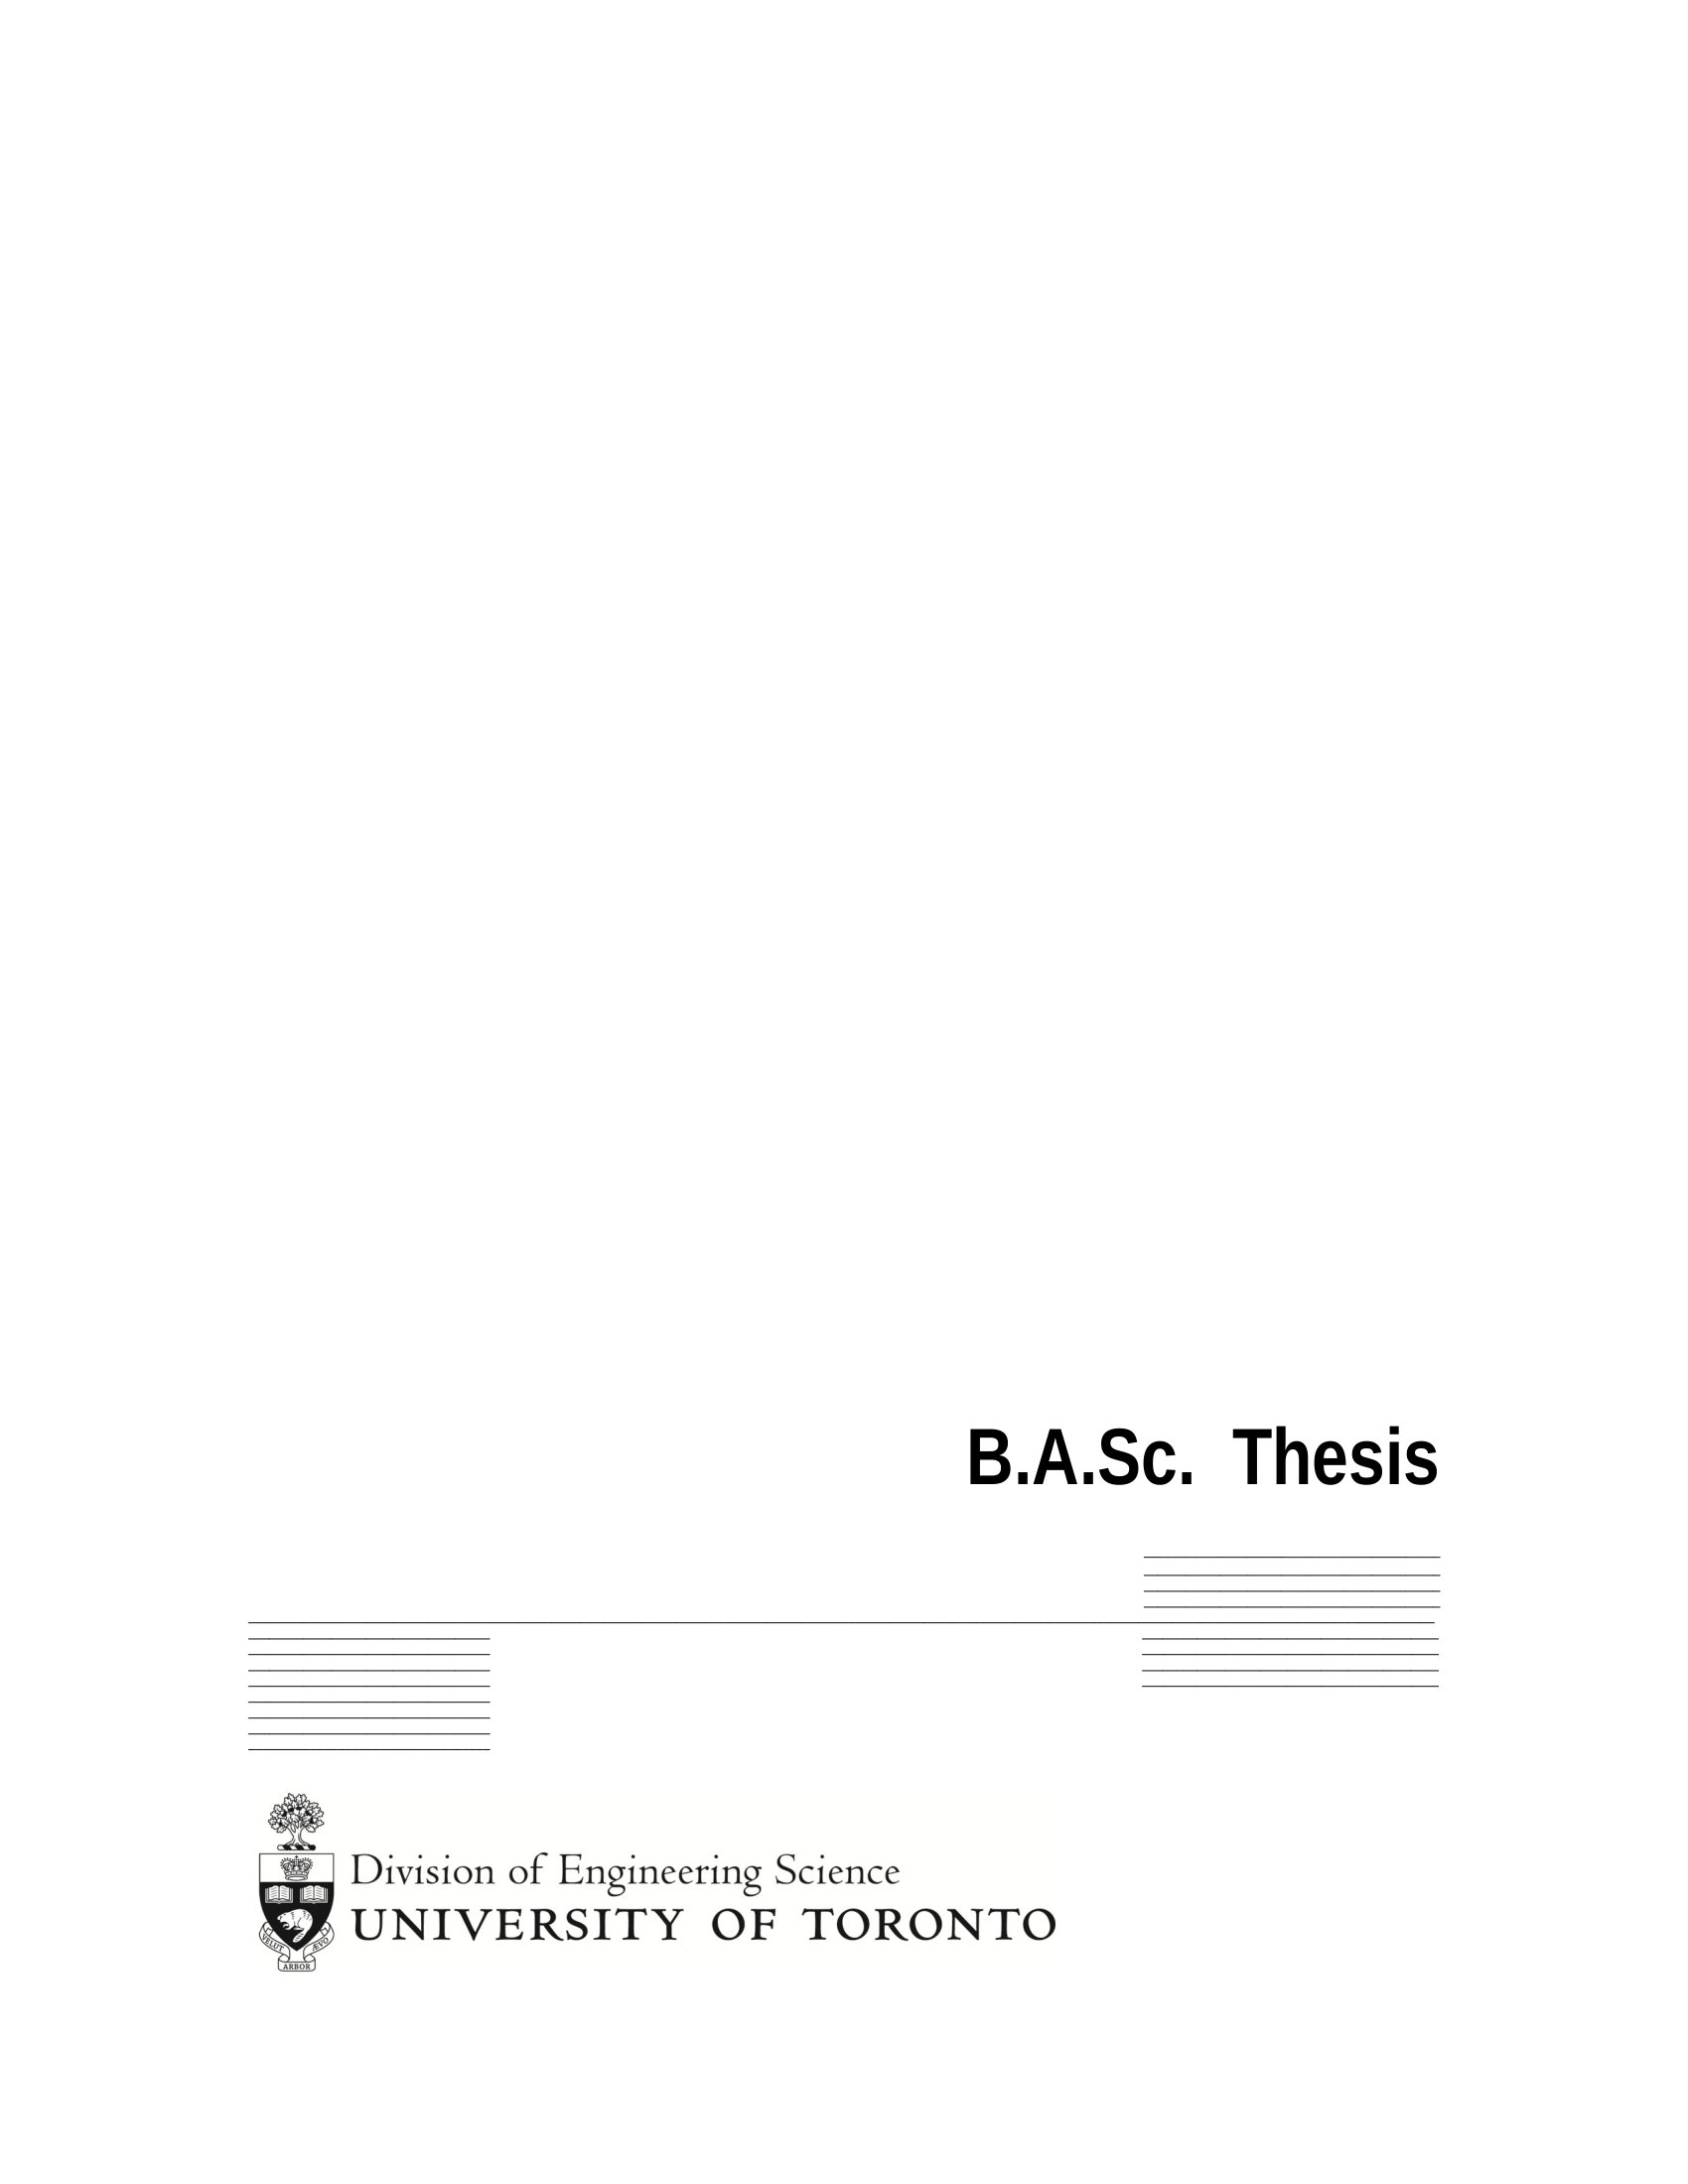
\includegraphics[width=\paperwidth,height=\paperheight]{images/cover.png}};
\clearpage
\pagebreak

\pagenumbering{roman}
\section*{Abstract}
\addcontentsline{toc}{subsection}{\protect\numberline{}Abstract}

Continuum robots prove difficult in modelling and control because of their extremely non-linear behaviour and complex modelling requirements. Traditional beam modelling methods are either computationally inefficient or are incapable of accurately controlling non-simulated robots, even ones that are well constructed. The added complexity of trying to model inaccuracies in robot construction makes controlling continuum robots challenging. Parallel continuum robots add the opportunity of higher applied forces to the compliant robots, but they only add to the complexity of the control problem. With the rise of machine learning many deep neural networks have been demonstrated effective in modelling complex relationships. In this work we take steps towards learning-based control of a planar parallel tendon-driven continuum robot. This work introduces a robot prototype designed to be a standard research platform for learning based control design for PCRs, a dataset collected with the intent of use in both state estimation and control tasks, two baseline controllers to use as a reference point for future learning based work, and several negative learning-based control experiment results to inform future work. The contributions in this thesis lay the foundations for learning-based state estimation and control for a parallel continuum robot. All project code is available freely at: \url{https://github.com/spencerteetaert/pcr_control}.

\textbf{Keywords}: parallel continuum robots, differential control, machine learning, learning-based control, benchmarks
\pagebreak
\section*{Acknowledgements}
\addcontentsline{toc}{subsection}{\protect\numberline{}Acknowledgements}

I would first like to thank Professor Burgner-Kahrs for the opportunity to pursue this research at CRL. This experience will be the foundation for my future academic work. Thank you to Reinhard Grassmann and Sven Lilge for guiding me through this project. They both provided a tremendous amount of help throughout the project both contributing to the work and guiding my goals in academia moving forward. Thank you to the one UTM shuttle bus driver who does not accept my ticket because "this school takes enough of your money". He really made my day during the weeks where it felt like nothing was working. Thank you to Callie Moore and Aidan Grenville, without whom I would have never made it through these last five years. Lastly, thank you to my dad. Though we disagree on many things, he has always been the one who encouraged me to be curious, to question why, and to figure things out for my own. 

\pagebreak  
\tableofcontents
\pagebreak
\section*{List of Symbols}
\addcontentsline{toc}{subsection}{\protect\numberline{}List of Symbols}

\newenvironment{tableofsymbols}
  {\par\vspace{\abovedisplayskip}\noindent\begin{tabular}{>{$}l<{$} @{${}={}$} l}}
  {\end{tabular}\par\vspace{\belowdisplayskip}}


\textbf{Abbreviations}
\begin{tableofsymbols}
\textit{CR} & Continuum Robot \\
\textit{TDCR} & Tendon-Driven Continuum Robot \\
\textit{PCR} & Parallel Continuum Robot \\ 
\textit{CC} & Constant Curvature (modelling assumption) \\
\textit{PID} & Position, Integral, and Derivative controller \\
\textit{RMSE} & Root Mean Squared Error \\
\textit{OL} & Open Loop (in controls) \\
\textit{CL} & Closed Loop (in controls) \\
\textit{DOF} & Degree Of Freedom \\
\end{tableofsymbols}


\noindent\textbf{Math Symbols}
\begin{tableofsymbols}
O_{ee} & End effector position [$\in \mathbb{R}^2$] \\
O_i & Arm base position [$\in \mathbb{R}^2$] \\
O_{goal} & Goal position [$\in \mathbb{R}^2$] \\
\ell_{ee, i} & Distance between base point and end effector point \\
\ell_{goal, i} & Distance between base point and goal point \\
l_t & Length of a tendon \\ 
\kappa_i & Arm curvature \\
\alpha_i & Arm angle \\
\varphi_i & Arm subtended angle \\
K_p & Controller proportional gain \\
K_d & Controller derivative gain \\
K_i & Controller integral gain \\
u & Control signal. Typically a position or velocity \\ 
q & Joint variable. Typically a motor rotation or angular velocity \\ 
\end{tableofsymbols}


\noindent\textbf{Robot Physical Constants}
\begin{tableofsymbols}
\ell_i & \SI{80}{cm}, Arm length \\
\ell_t & \SI{11}{mm}, Distance between the beam and the tendon \\ 
G & 64, Motor gear ratio \\ 
r_m & \SI{11}{mm}, Tendon spindle radius \\
\end{tableofsymbols}


\pagebreak
\listoffigures
\addcontentsline{toc}{subsection}{\protect\numberline{}List of Figures}
\pagebreak
\listoftables
\addcontentsline{toc}{subsection}{\protect\numberline{}List of Tables}
\pagebreak

\pagenumbering{arabic}
\section{Introduction}

Continuum Robots (CRs) are a current topic of research because of their inherent compliance, ability to be manufactured on sub-millimeter scales, and ability to have non-linear shape deformations \cite{4058827, survey}. This makes them ideal robots to be used in surgical and inspection applications \cite{7314984, DONG2017218}. Because of a CR’s compliance, it is limited in the force it can exert on the environment through a given end effector. Parallel Continuum Robots (PCRs) see multiple CRs attached at a common end effector, maintaining system compliance while enabling the robot to apply higher forces to the environment \cite{6906943, survey}. 

Forward and inverse kinematic modelling of a robot can be used in model-based control to move a robot with specified motions. Static modelling allows for the consideration of forces while dynamic modelling considers temporal effects on the system. Current models of CRs are unable to account for a number of complex factors in the system, such as internal robot friction, surface friction, and external loads, without significant computational overhead \cite{10.3389/frobt.2020.630245}. To achieve computation speeds that enable real-time control, often assumptions are made to simplify the robot’s static model to a simple kinematic one \cite{9143427} or to represent the robot's state with geometric approximations \cite{10.3389/frobt.2020.630245, 9143427, slilge_2020}. These simplifications greatly improve computation time while sacrificing model predictive accuracy. It is desirable to have the means to model these systems in real-time without making accuracy-sacrificing assumptions that seldom hold true in real-world applications.

Machine learning approaches have promised faster results and more accurate approximations of complex systems \cite{9199280}. Several works have demonstrated learning-based systems and their value to both the control and state estimation tasks \cite{s21062085, 8972568, 8643440, doi:10.1146/annurev-control-090419-075625, TOQUICA2021106682}. It is therefor a natural next step for PCRs to take advantage of the advantages of learning-based solution to help address the shortcomings of existing approaches. While some work has been done to use learning in CR control \cite{10.3389/frobt.2021.730330, grassmann2022a, 7112506}, nothing has been proposed for PCRs. 

\subsection{Contributions}
To achieve learning-based control for this system while ensuring future works have an accurate comparison point, several foundational steps must be taken. This thesis takes several of those steps to advance the field of CRs towards learning-based solutions. The contributions of this thesis are:
\begin{enumerate}
    \item Re-design and validation of a prototype for a two DOF planar parallel tendon-driven continuum robot. The robot is designed as an easy to implement research platform by using off-the-shelf components and 3D printed parts and being built for modularity and rapid reconfiguration  
    \item Establishes two real-time baseline controllers utilizing PID control and the constant curvature assumption that satisfy a \SI{1000}{Hz} update rate and have zero closed-loop asymptotic tracking error in task space  
    \item Establishes a data set for both control and state estimation tasks in addition to providing a learning-based pipeline for these tasks
    \item Presents several negative learning-based control results to inform future work 
\end{enumerate}

% The project was started with the redesign of an existing planar parallel tendon-driven continuum robot initially constructed at the Continuum Robotics Lab \cite{crl}. The robot was prototyped and manufacturing began but the model was never completed or tested. As the robot was partially completed at the start of this thesis, justification for some of the design choices of this particular robot is outside of the scope of this report. Completion and validation of the physical prototype is the first major objective of this thesis. 

% Establishing a baseline controller serves to act as both a comparison point to the learning-based controller and to enable reasonable control of the robot for data collection. A baseline model has been developed using techniques consistent with other works in the CR field. Evaluation of the effectiveness of this baseline controller must be completed for use as a reference for future approaches. 

% Future work will explore the development and evaluation of a learning-based controller for the robot prototype to compensate for unmodelled effects in the kinematic model of a planar parallel continuum robot \cite{slilge_2020}. Learning makes sense in this scenario due to its relatively low computation time to approximate complex models. Data will be collected on the physical system by generating a sample of control inputs and recording the end effector position and motor feedback over time. Trajectories will be restricted to enforce $C^4$ smoothness \cite{8772208} to be in line with standard robotics practice. Collection of end effector position data will follow the procedure in \cite{grassmann2022a} and collection of motor feedback as in \cite{Grimminger_2020}. 

\subsection{Document Structure}
In Section \ref{sec:background} a background of concepts is provided alongside a review of current state-of-the-art modelling methods. Section \ref{sec:methods} describes the robot prototype, baseline controller derivations, and dataset generation methodology. Section \ref{sec:results} will present the results of the four aspects of this project. Section \ref{sec:discussion} will explore the significance of the experiment results and highlight the limitations of this project. Lastly, Section \ref{sec:conclusion} will explore potential future work that could follow the proposed work. 
\pagebreak
\section{Background}
\label{sec:background}
In this section we consider a portion of available literature on both CRs and control to motivate the use of learning-based control for the PCR considered in this work. As learning-based control for a PCR configuration has not yet been studied in the available literature, the scope of this section is only to provide a background of relevant topics and not a comprehensive review of all available control and modelling methods. 


\subsection{Types of Continuum Robots}
CRs can be defined as "an actuatable structure whose constitutive material forms curves with continuous tangent vectors." \cite{7314984} CRs are robots with an infinite number of joints and degrees of freedom. By using flexible components, CRs are inherently compliant, making them useful in applications where interactions with stiff joints may cause damage to the environment. They are also able to be manufactured on sub-millimeter scales. As such, these robots have seen use in medical and inspection applications \cite{7314984, DONG2017218, 4058827}. Continuum robots come in a variety of configurations, materials, and actuation methods \cite{doi:10.34133/2022/9754697}. Modelling methods for continuum robots are discussed in Section \ref{sec:modelling_methods}. The subset of continuum robots pertaining to this thesis is considered.  

\begin{figure}[H]
    \centering
    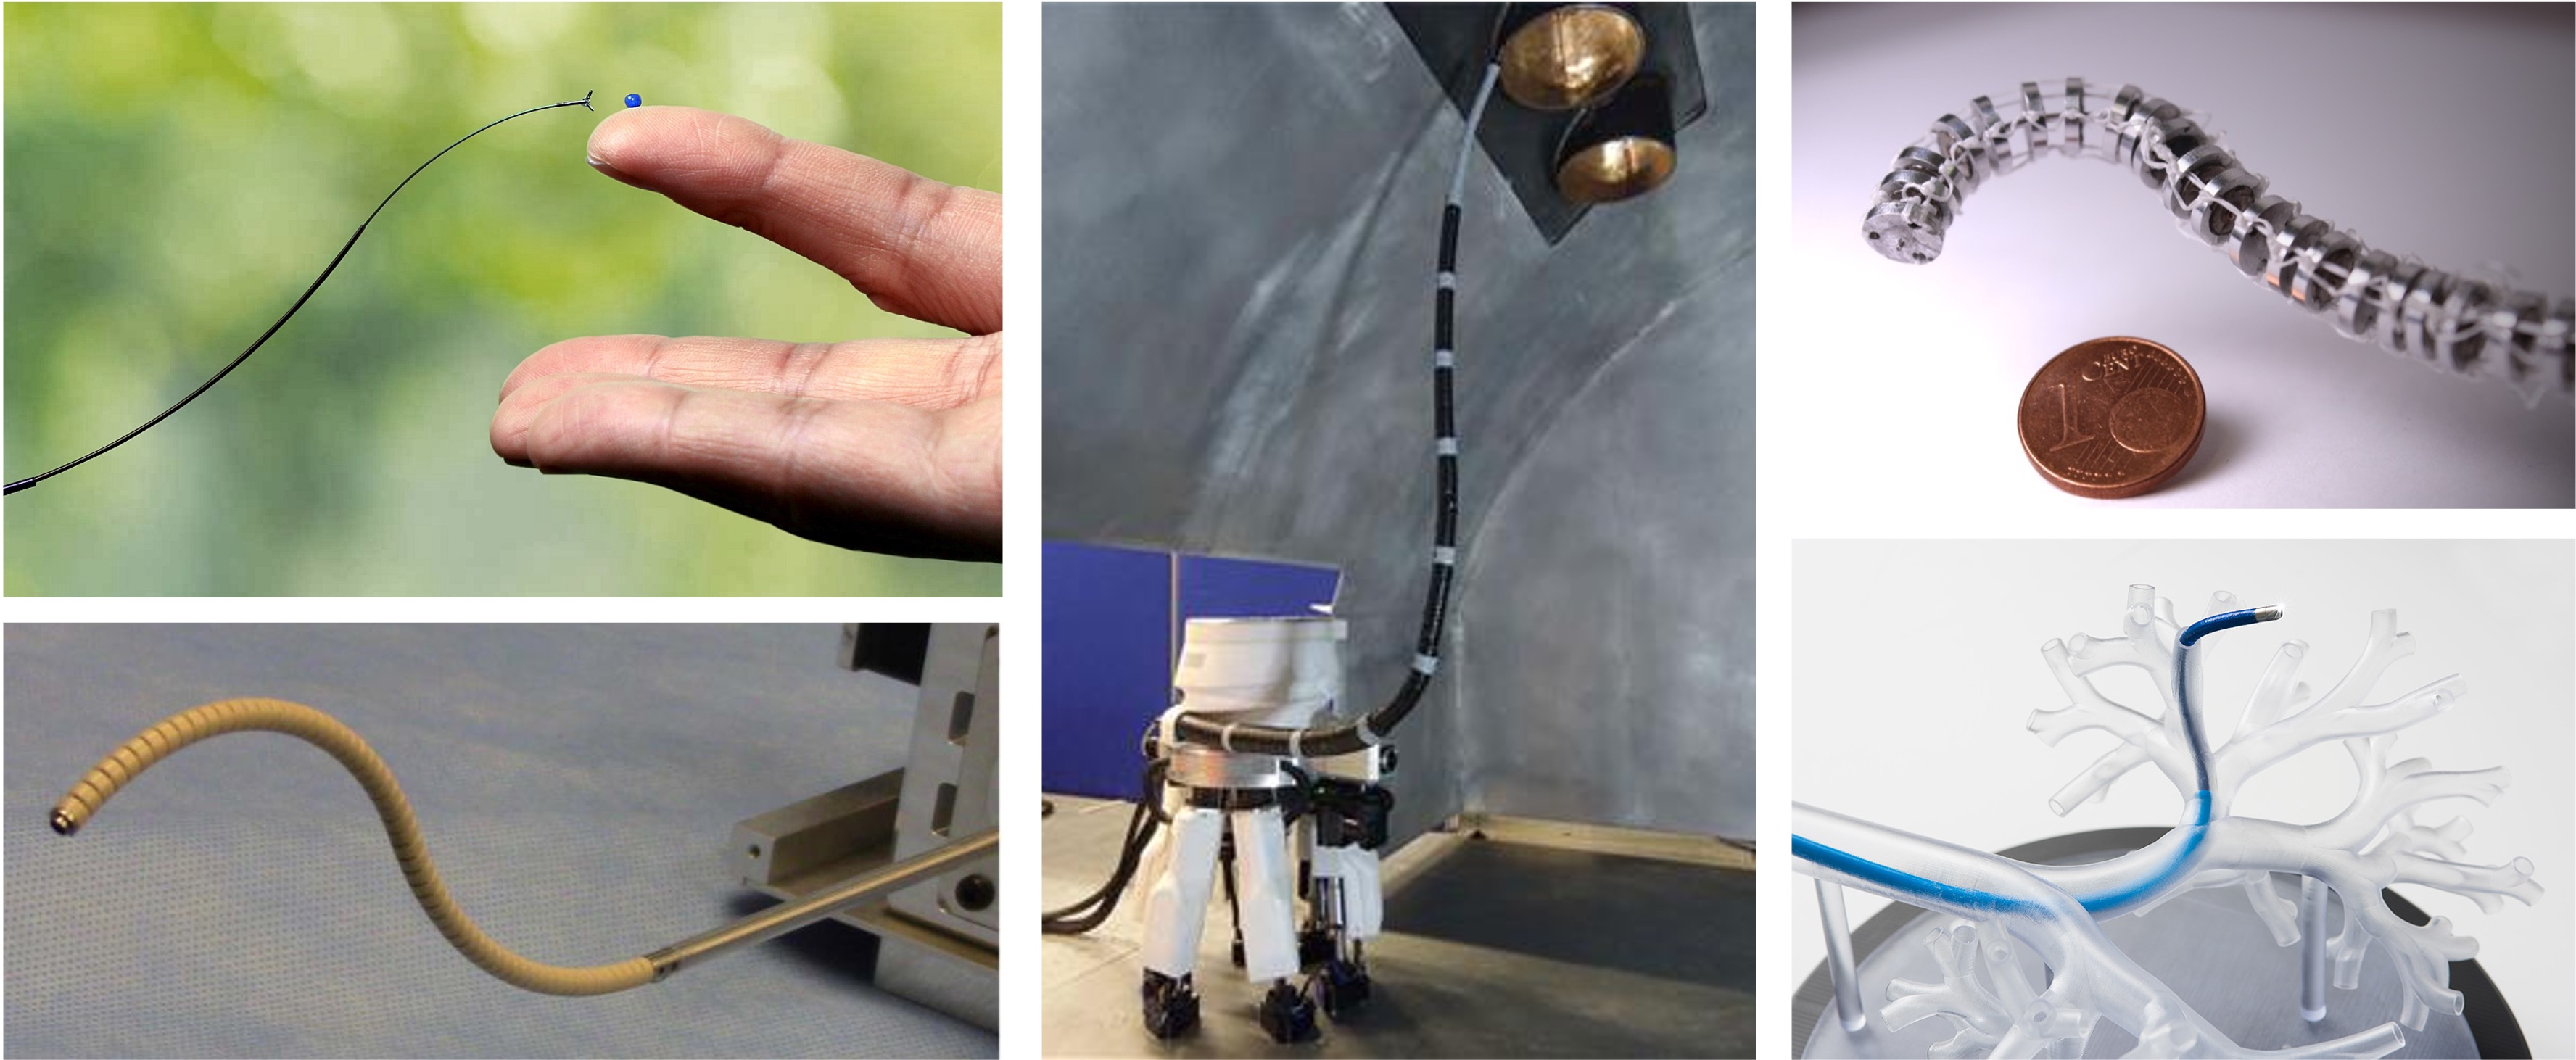
\includegraphics[width=\textwidth]{images/cr_examples.jpg}
    \caption{Continuum robot examples, from \cite{crl_cr_types}}
    \label{fig:cr_examples}
\end{figure}

\subsubsection{Tendon-Driven Continuum Robots}
Tendon-Driven Continuum Robots (TDCR) are a class of CRs that are actuated by contracting a tendon that is attached to a point along the robot's backbone. The backbone is typically a highly elastic rod or beam that provides stiffness to the robot while remaining compliant. The tendon is constrained to be a fixed distance from the backbone by a series of spacer disks. Contracting the tendon results in the backbone bending towards the side the tendon is offset on \cite{HEMAMI198527, 10.3389/frobt.2020.630245}. An "arm" of a TDCR refers to a single beam that can be actuated independently of other arms in the robot. 

\subsubsection{Parallel Continuum Robots}
PCRs use multiple arms joined together to increase the stiffness and maximum applied force of a CR while maintaining the inherent compliance that CRs have to offer \cite{survey}. 

\subsubsection{Robot Configurations}
PCRs can take on a wide variety of configurations. In \cite{6906943}, a six-beam PCR is proposed and modelled based on Cosserat rod theory. Flexible rods are translationally pushed and pulled to achieve actuation. A tracking accuracy of 2.89\% of the length of one arm of the robot was achieved.  \cite{slilge_2020} introduces a three-beam parallel TDCR with six degrees of freedom at the end effector. The authors model each beam using a geometric kinematic model based on the constant curvature assumption. A planar configuration reduces the task space to a 2D plane. These robots have at most three degrees of freedom at the end effector; two spatial components and a rotational one. In \cite{9143427}, a planar PCR is proposed along with a geometric model controller based on the constant curvature assumption. It achieves an accuracy of 1\% of the length of one arm of the robot.  


\subsection{Modelling Continuum Robots}
\label{sec:modelling_methods}
It is desirable to construct a forward and inverse kinematic model when controlling a robot. A forward kinematic model provides an expression for the end effector position given a robot's joint variables. It is used to estimate the end effector position of a robot during operation when direct measurements are not available. An inverse kinematic model solves for a robot's joint variables given a desired end effector position. It is used in control tasks to move the robot into a desired configuration. In both cases, the accuracy of the model is determined by a number of factors including the simplifying assumptions made in exchange for increased computational efficiency \cite{10.3389/frobt.2020.630245}. Figure \ref{fig:timing_from_source} demonstrates the run time benefit from using models that make simplifying assumptions and the sacrifice that is made in terms of accuracy. 

\begin{figure}[h]
    \centering
    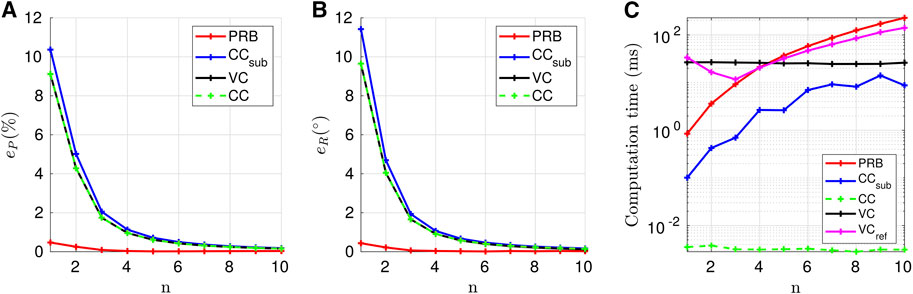
\includegraphics[width=\textwidth]{images/time_graph_from_survey.jpg}
    \caption{Timing analysis of pseudo-rigid body, constant curvature, and variable curvature modelling methods in a simulated environment, from \cite{10.3389/frobt.2020.630245}}
    \label{fig:timing_from_source}
\end{figure}

There are three major types of robot models that we consider: (1) kinematic models, (2) static models, and (3) dynamic models. Kinematic models model the shape of the robot without consideration of forces. Static models consider the robot at points of equilibrium, where the robot is not moving and has zero net force. Dynamic models model the robot as it's moving, accounting for transient effects (such as spring forces, friction, air resistance, etc.). 

In rigid robotics, simple linear models exist that accurately model the robot's motion. CRs do not have such a luxury due to their non-linear deformation. As such, more system assumptions or more complex models must be used for even the simplest of CRs \cite{10.3389/frobt.2020.630245}. As this is an emerging research field, the accuracy of models for CRs is not yet comparable to conventional industrial robots. 

\subsubsection{Constant Curvature Assumption}
The most common and convenient kinematic modelling approach for continuum robots uses the constant curvature (CC) assumption \cite{doi:10.1177/0278364910368147}. It assumes that the curvature throughout the entire length of an arm is constant. This assumption greatly reduces the complexity of the forward and inverse kinematic models of a continuum robot. 

\paragraph{Euler Beam Theory}
Euler beam theory can be used to create a static model assuming that the effects of shear and twist are negligible \cite{10.3389/frobt.2020.630245}. The CC assumption allows for computationally efficient implementations of the inverse kinematics problem. It does however result in a number of inaccuracies as beams under high bending do not have CC. Modelling a continuum robot using the CC assumption and Euler beam theory has been shown to result in poorer accuracy compared to using a variable curvature model \cite{10.3389/frobt.2020.630245}.

\subsubsection{Variable Curvature Representation}
Without losing generality, one can model the curvature of a continuum robot using a variable curvature representation. This representation makes no assumptions about the backbone shape as it can model any point along it with six degrees of freedom \cite{10.3389/frobt.2020.630245}.  

\paragraph{Cosserat Rod Theory}
The Cosserat theory of elastic rods extends the variable curvature kinematic representation into a static model. Modelling in this way accounts for shear deformations, something Euler beam theory did not. While the Cosserat rod theory approach has been shown to produce excellent accuracy in continuum robot applications \cite{10.3389/frobt.2020.630245, CAO2008460, ALQUMSAN201948, 10.1007/978-3-319-64107-2_56}, it does so at great computation costs, resulting in the inability to be used for real-time control \cite{10.3389/frobt.2020.630245, ALQUMSAN201948}. A number of implementations for the cosserat theory model have been realized with accuracies ranging from 12\%\cite{10.1007/978-3-319-64107-2_56} to \SI{4e-10}{m} - \SI{8e-10}{m} Root Mean Squared Error (RMSE) for a robot of length \SI{30}{cm}\cite{ALQUMSAN201948}. 


\subsection{Machine Learning}
Machine learning has emerged as a useful tool for estimating complex functions using data collected from a system. In robotics, learning has been used to develop controllers for complex systems that are difficult to model. Deep learning approaches have shown promise in modelling complex dynamic behaviour for controller design in robotics \cite{9199280}. Because data-driven approaches can estimate arbitrarily complex functions \cite{HORNIK1989359} they are thought to be useful in continuum robots. Learning-based applications in continuum robotics have primarily focused on learning the inverse statics and kinematics of a robot \cite{10.3389/frobt.2021.730330}. With each of the results reviewed here, one must be weary of directly comparing results directly as large variations in performance can arise from changes in robot configuration, actuation type, and construction. In each of the works reviewed, the proposed learning-based model outperformed baseline approaches on the same robot.

\subsubsection{In Continuum Robotics}
\paragraph{Data-driven approaches}
 In \cite{8115276}, the authors use a model-free approach using an adaptive Kalman Filter. This uses sensor data to update the model's uncertainty estimations during operation, resulting in a more controller that had an experimental tracking RMSE of \SI{1.52}{mm} (with a \SI{20}{cm} - \SI{25}{cm} long pneumatic continuum robot). In \cite{rcs.1774}, the authors implement three regression models to learn the inverse kinematics of a flexible surgical robot, achieving a top RMSE of \SI{2.1275}{mm} with a KNN regression. The authors do not report the total robot length. 

\paragraph{Deep learning approaches}
For deep learning approaches to work, a large amount of data or an accurate simulation environment must be available. As the dynamic effects of a continuum robot are what is difficult to model, simulation environments are not readily available. In \cite{grassmann2022a}, a dataset is released for concentric tube continuum robots. The authors propose a baseline learning model that achieves tip tracking errors of \SI{0.74}{mm} (or 0.4\% of the robot's length).  Using deep neural networks for approximating the inverse statics equation is the approach used in \cite{7112506}. The authors are able to achieve errors of around \SI{7}{mm}\footnote{Number, as reported, is an estimation by the thesis author. See reference paper for complete results breakdown.} for an underwater soft continuum robot (or about 2.5\% of the robot's length). For both of these implementations, a large amount of data is required that maps the robot's end effector position to its joint configuration, marking a large drawback to deep learning-based models. 

\subsubsection{In Other Robotics}
Although learning-based solutions are limited in their applications to CRs, they have been deeply explored in other robotics in areas that may be applicable to CRs such as sensing \cite{8643440, 9001195}, state estimation \cite{s21062085, 8972568, 8643440}, and control \cite{doi:10.1146/annurev-control-090419-075625, TOQUICA2021106682}. Each of these aspects have had results that demonstrate learning-based solutions and their ability to replace more conventional methods. Often however, hybrid approaches that make use of conventional modelling methods that are augmented using learning are shown to have the best results. 

In \cite{s21062085}, the authors highlight several elements in deep learning that prove useful in state estimation including the use of long short-term memory (LSTM) layers to enable long-term correspondence between input data, the use of Bayesian modelling to help account for complex system noise, and applying attention mechanisms to learn what is important and unimportant in the input data at each time step. The survey goes on to highlight the value in hybrid approaches that integrate learned systems with model-based approaches. The authors in \cite{8972568} take this one step further by demonstrating the hybrid approach on a manipulation task with a deformable object. The authors show that they can accurately estimate a rope's full state using a self-supervised deep learning network trained on image data. 

Robotic systems rely on their sensor data as the basis for state estimation. This data is generally corrupted by some amount of noise. \cite{8643440} demonstrates the use of deep learning to explicitly account for system noise in attitude estimation of a UAV. The authors in \cite{9001195} propose a pipeline for explicit handling of uncertainty caused from noisy inputs. They demonstrate their approach's success in robotic applications by estimating model uncertainty by propagating noise through the model and quantifying the effect. 

For learning-based control, \cite{doi:10.1146/annurev-control-090419-075625} highlights how neural networks can improve results in model predictive control (MPC). It looks at three different applications including using learning to model system dynamics and using learning to enhance objective function design. In \cite{TOQUICA2021106682}, deep learning is used to solve the inverse kinematic problem for a rigid parallel industrial robot. The work shows that deep learning based inverse kinematic solutions have applications in parallel robotics, boasting a 99.8\% accuracy compared to the analytical model. 


\subsection{Summary}
PCR design is still an open area of research. Work has focused on the benefits of these robots in their relevant application spaces. Research modelling and control for CRs have largely focused on single-beam CRs. A research gap exists for modelling and control of PCRs that is unaddressed by current classical modelling methods. Significant modelling assumptions that ignore dynamic effects of the system or make inaccurate claims about the kinematic description of the system allow for fast but inaccurate control. When these assumptions are not made, controllers have infeasible computation speeds for real-time control. Data-driven approaches may be able to solve this problem but are underdeveloped for parallel continuum robots. This thesis aims to address this gap by taking steps towards learning-based control for a planar parallel TDCR. 
\pagebreak
\section{Methods}
\label{sec:methods}

\begin{figure}[H]
    \centering
    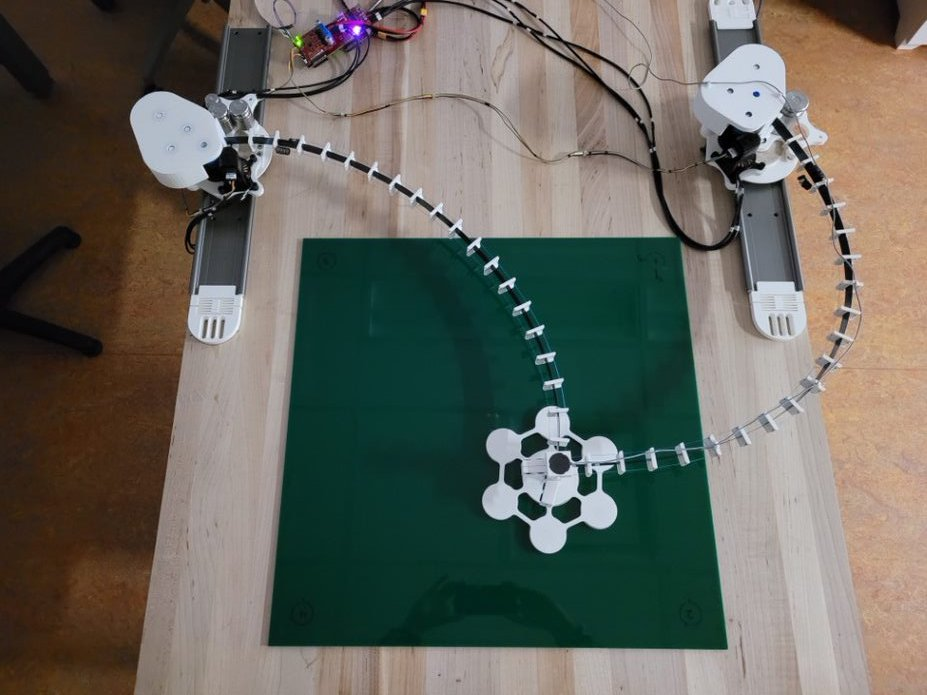
\includegraphics[width=0.7\textwidth]{images/current_setup.jpeg}
    \caption{Prototype setup}
    \label{fig:prototype}
\end{figure}

\subsection{Prototype Hardware}
% Add drawings / design philosophy 
The robot is designed with the Open Continuum Robotics project in mind. It uses easily accessible, off-the-shelf components, and 3D printed parts so that other groups can reconstruct the same robot. A full breakdown of the robot's physical design can be found in Appendix \ref{app:robot_drawings}. 

\subsubsection{Physical Description of Prototype}
\label{sec:physical_description}
% Arms
\paragraph{The arms} are each \SI{80}{cm} long and consist of a \SI{0.0200}{"} thick, \SI{0.75}{"} wide beam made from 1095 spring steel, with 19 evenly spaced 3D printed tendon spacers. The spacers hold one tendon on each side of the beam \SI{11}{mm} away from the steel beam. The 1095 spring steel beam is used as the central beam as it provides rigidity in the direction of motion off the robot's planar surface, while remaining flexible along the plane. The high elasticity of the material allows the system to undergo large curvatures without permanently deforming the beam. The tendons used are \SI{30}{lbs} braided fishing line (Super8Slick V2, Power Pro, CA, USA). Each tendon has four \SI{0.75}{"} nuts on it that act to maintain tension during operational periods where it is being extended. 

\begin{figure}[h]
    \centering
    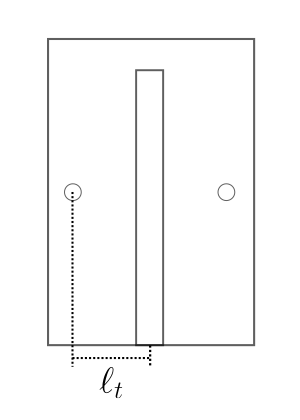
\includegraphics[width=0.3\textwidth]{images/beam_cross_section.png}
    \caption{Cross section of the beam spacers. $\ell_t = \SI{11}{mm}$}
    \label{fig:beam_cross_section}
\end{figure}

\begin{figure}[h]
    \centering
    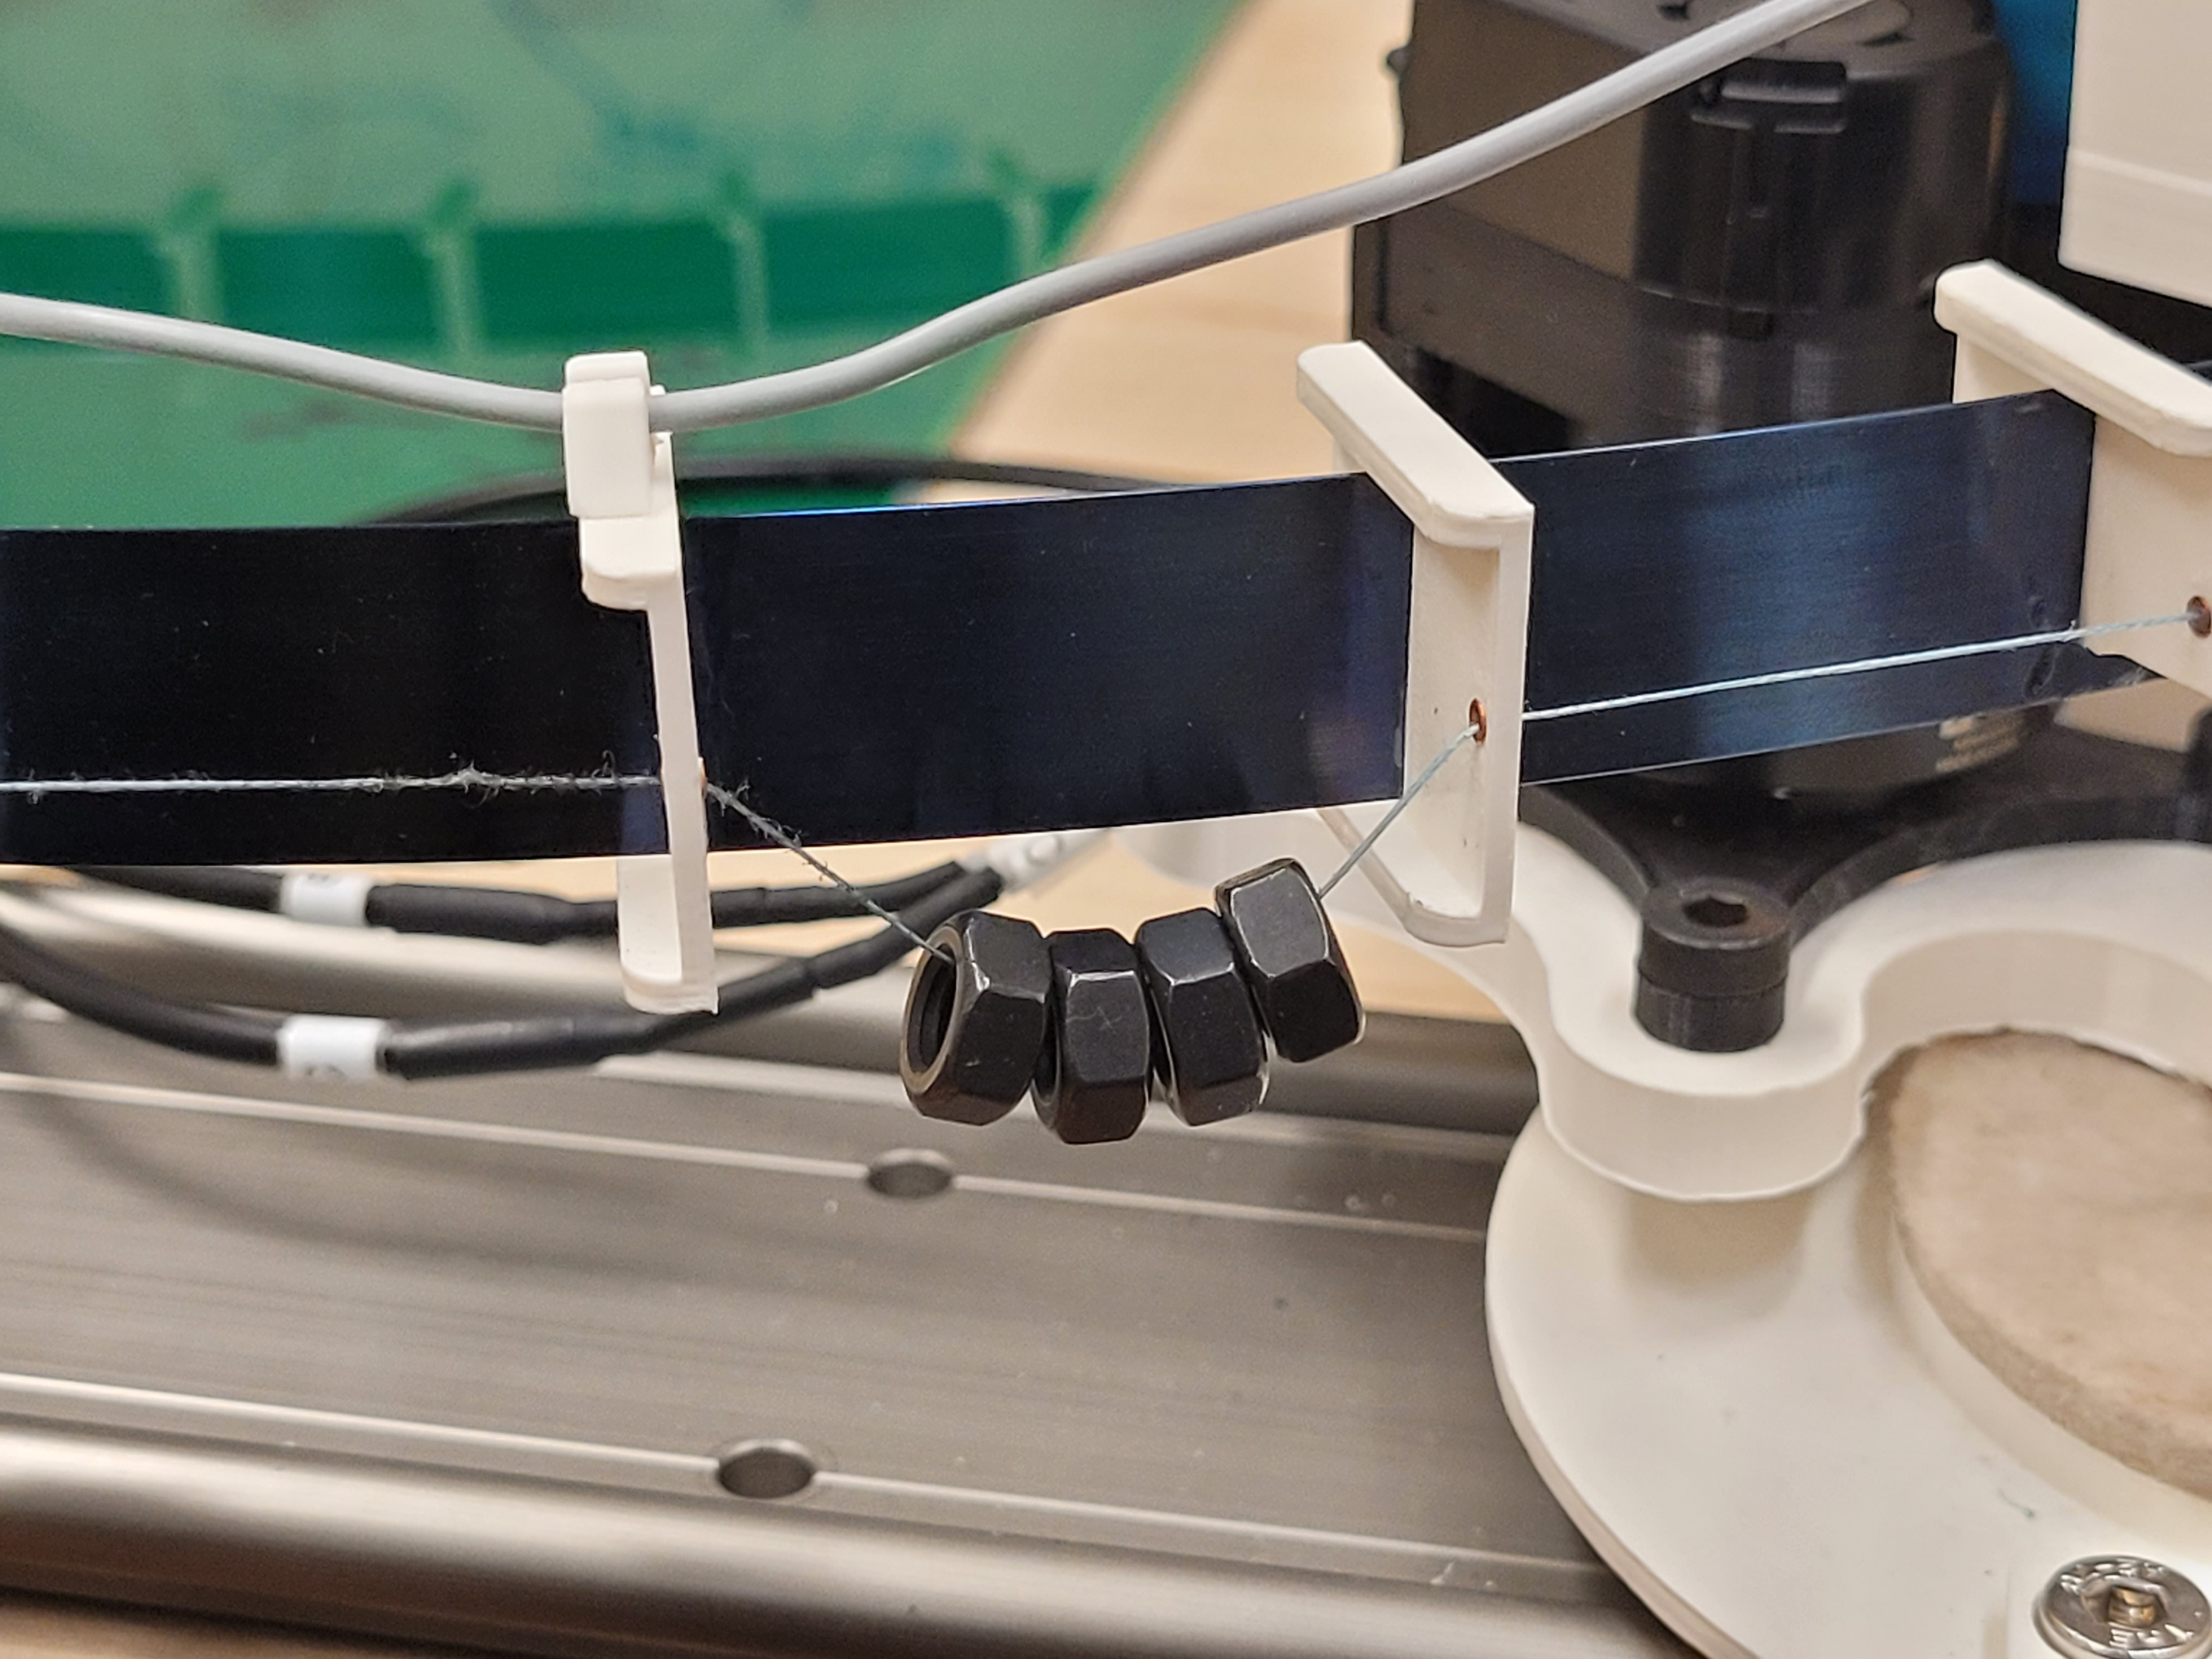
\includegraphics[width=0.5\textwidth]{images/tendon_slack.jpg}
    \caption{Four \SI{0.75}{"} nuts placed on a tendon to maintain tendon tension throughout operation}
    \label{fig:tendon_slack}
\end{figure}

% \begin{figure}[h]
%      \centering
%      \begin{subfigure}[b]{0.48\textwidth}
%          \centering
%          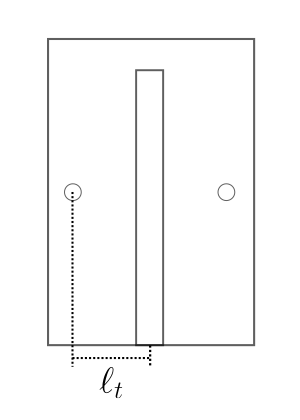
\includegraphics[width=0.625\textwidth]{images/beam_cross_section.png}
%          \caption{Cross section of the beam spacers. $\ell_t = \SI{11}{mm}$}
%          \label{fig:beam_cross_section}
%      \end{subfigure}
%      \hfill
%      \begin{subfigure}[b]{0.48\textwidth}
%          \centering
%          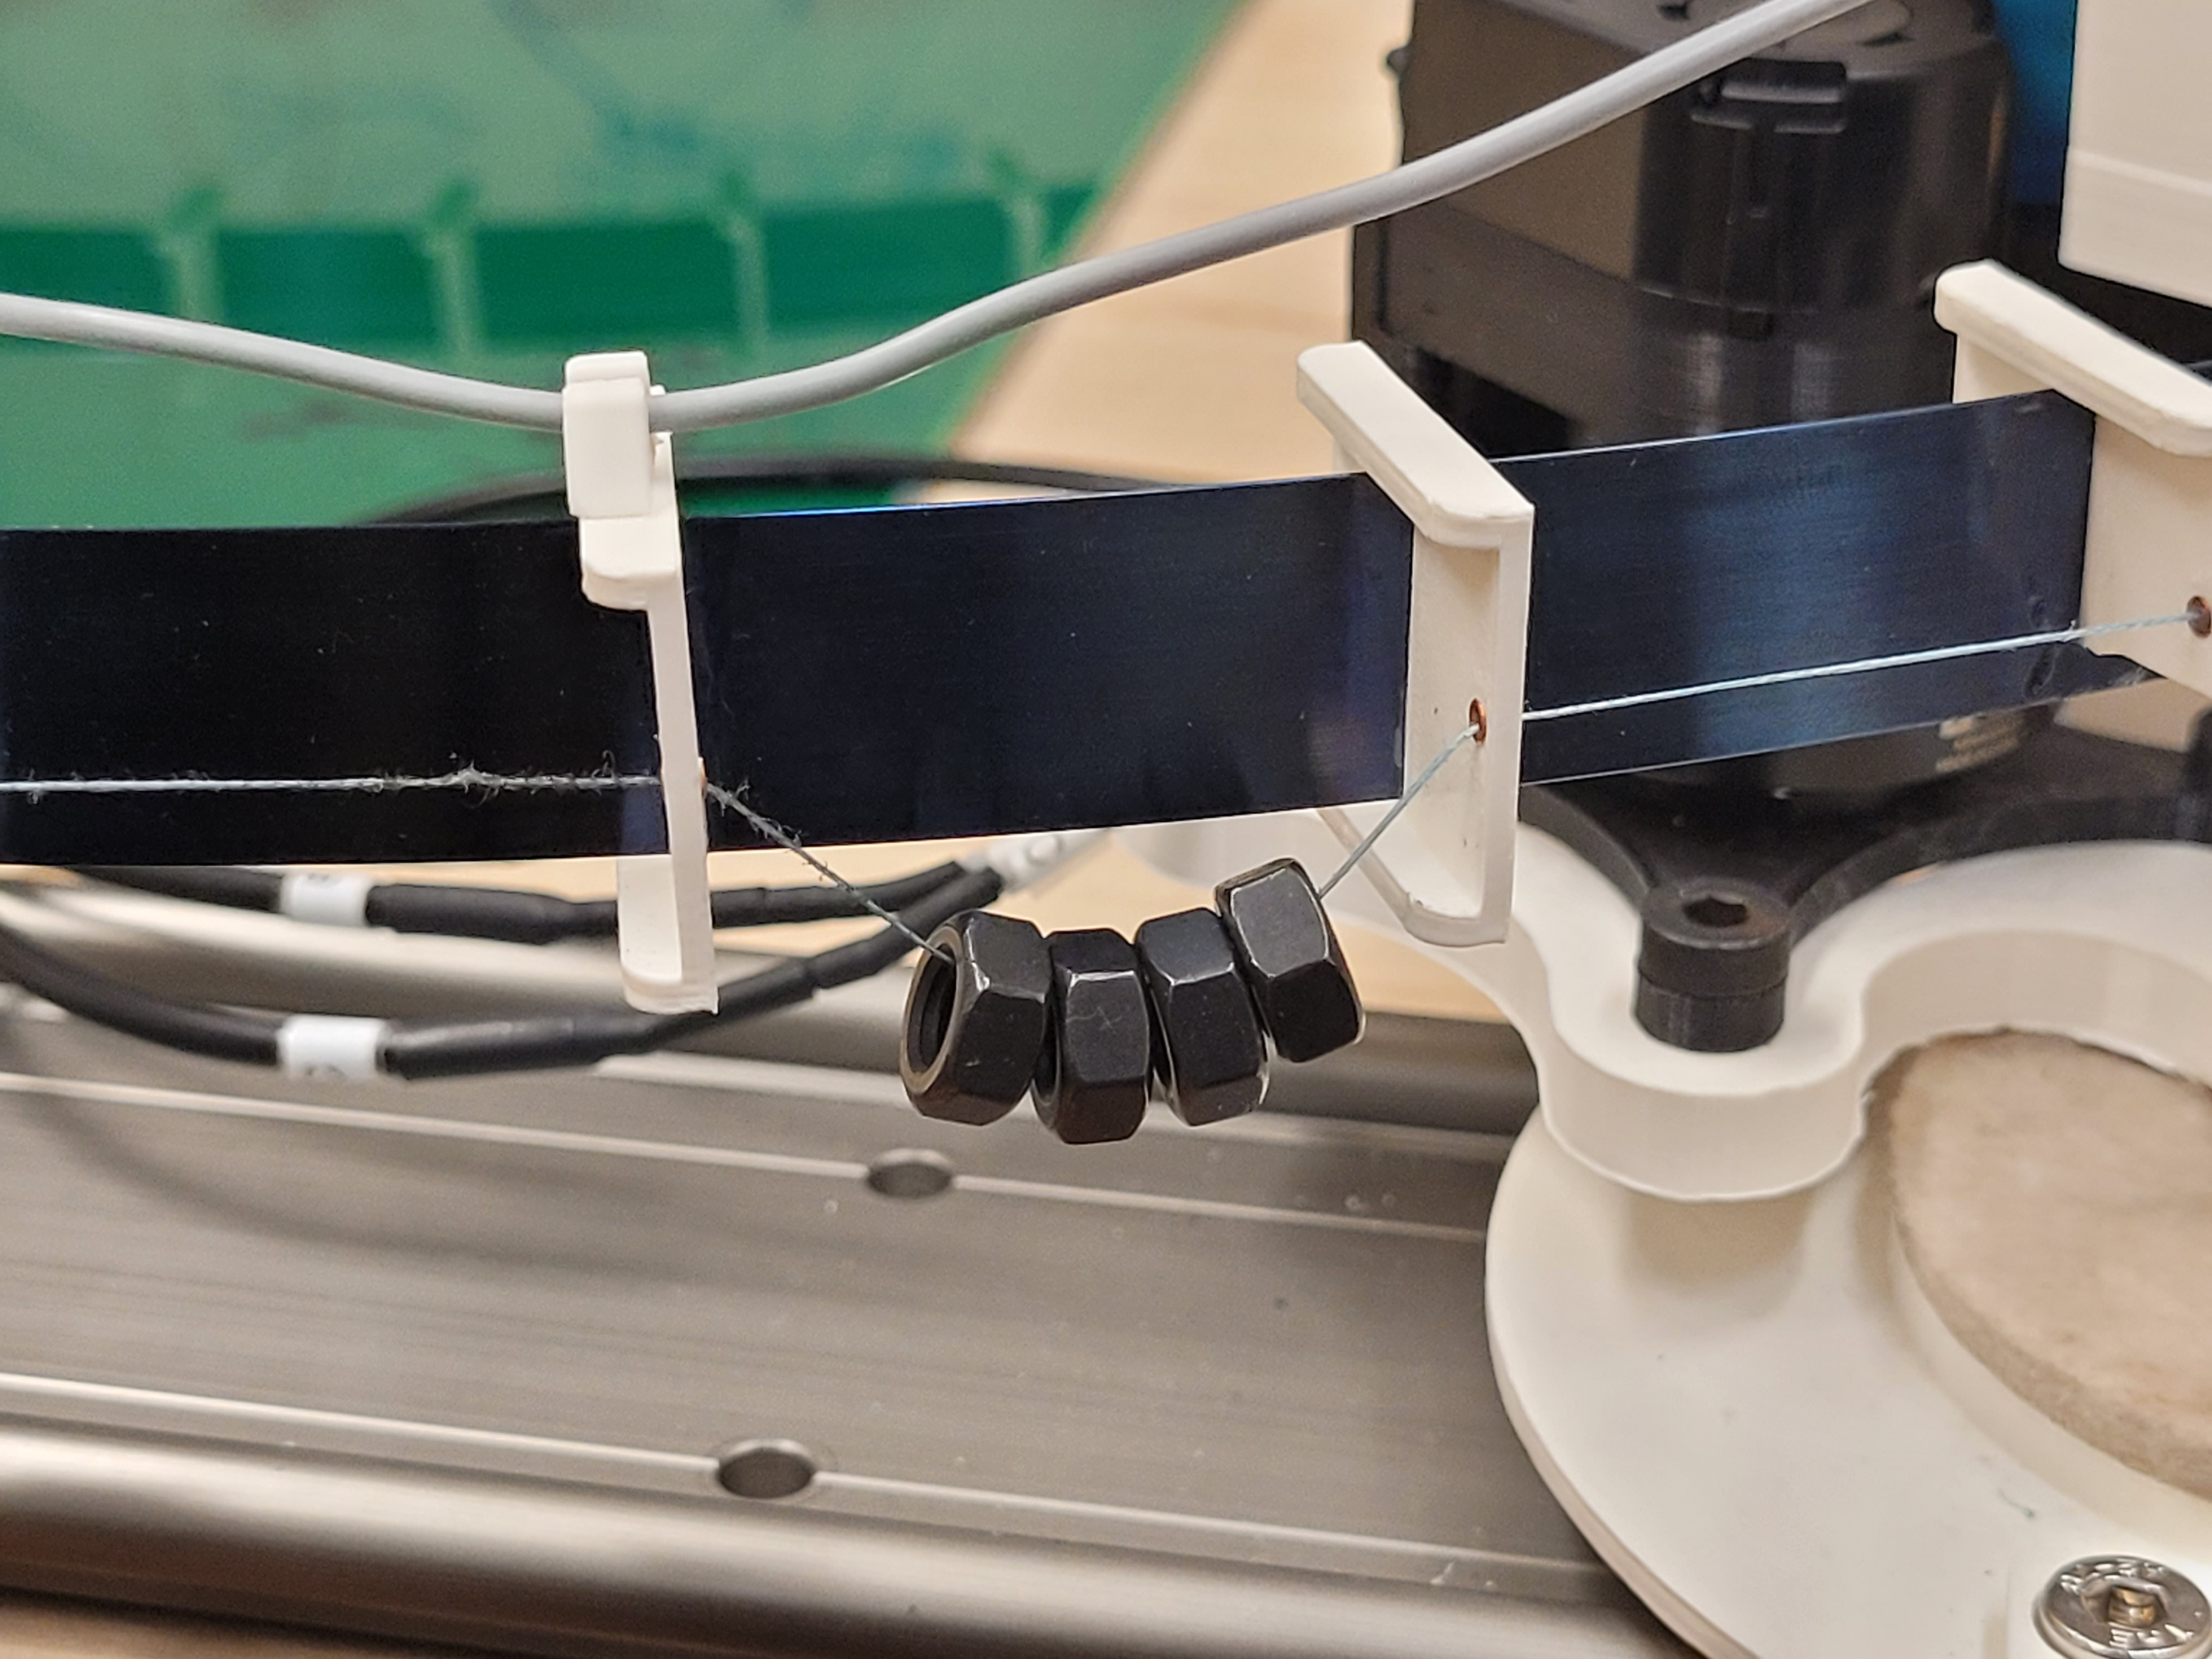
\includegraphics[width=\textwidth]{images/tendon_slack.jpg}
%          \caption{Four \SI{0.75}{"} nuts placed on a tendon to maintain tendon tension throughout operation}
%          \label{fig:tendon_slack}
%      \end{subfigure}
% \end{figure}

% Joints and End Effector  
\paragraph{The end effector} features a wide base to prevent the end effector from twisting off the plane. Revolute joints link the ends of each arm to the motor bases and the end effector, allowing both ends to rotate freely about the z-axis. The two arms share the same end effector. The bases for each arm are positioned \SI{60}{cm} apart.Each arm having its own independent degree of freedom grants the end effector in this configuration two degrees of freedom laying on the table plane. At this distance, the reachable workspace of the end effector covers a majority of the AURORA tracker workspace. During operation, a smaller end effector base does not provide enough area to balance the moments being applied by the two arms actuating the piece from different heights. Figure \ref{fig:ee_comparison} demonstrates this effect in action. Felt pads are attached to the bottom of the end effector to reduce friction between the end effector and table surface. 

\begin{figure}[h]
     \centering
     \begin{subfigure}[b]{0.48\textwidth}
         \centering
         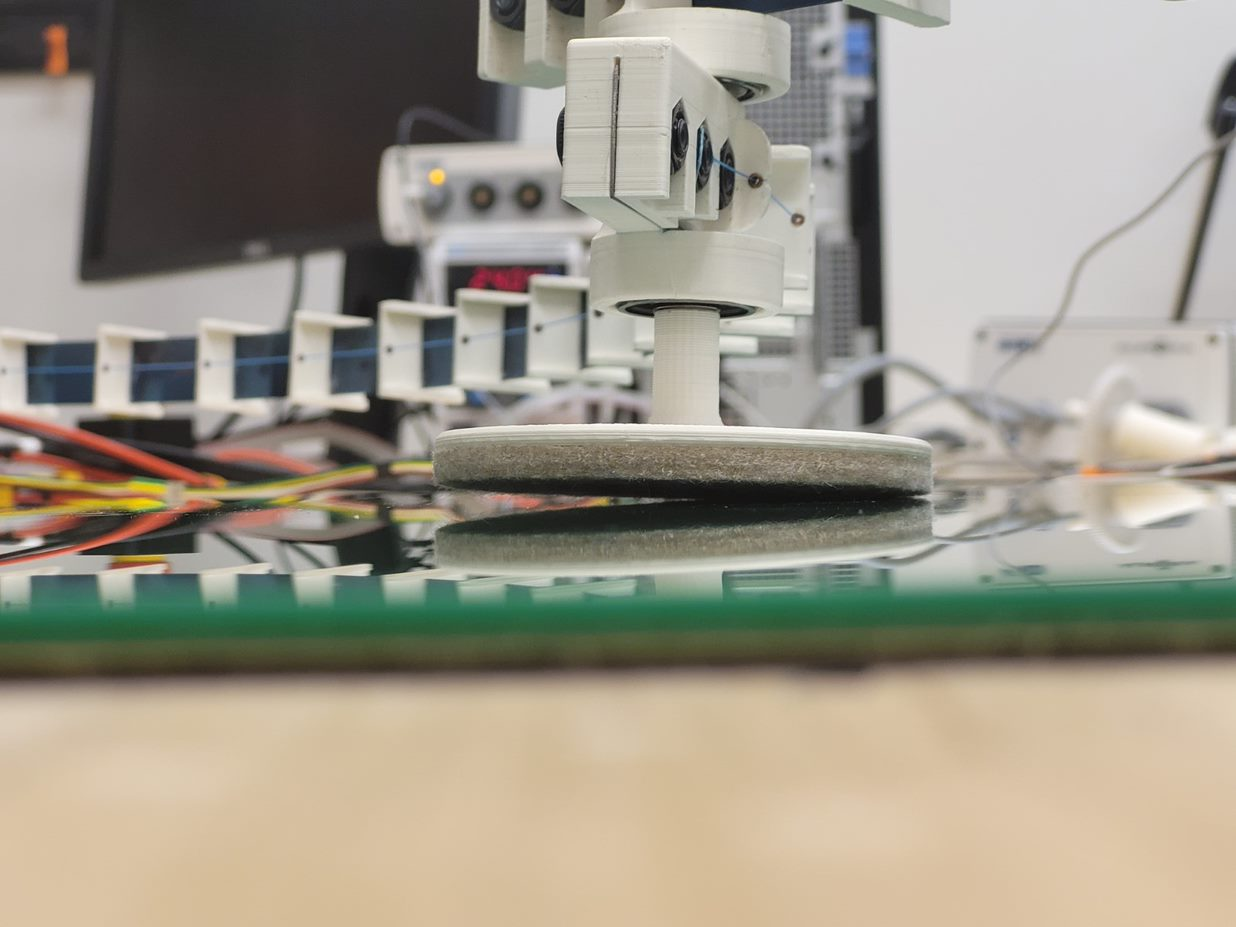
\includegraphics[width=\textwidth]{images/small_ee.jpeg}
         \caption{Smaller base causing the end effector to twist off the planar surface}
         \label{fig:small_ee}
     \end{subfigure}
     \hfill
     \begin{subfigure}[b]{0.48\textwidth}
         \centering
         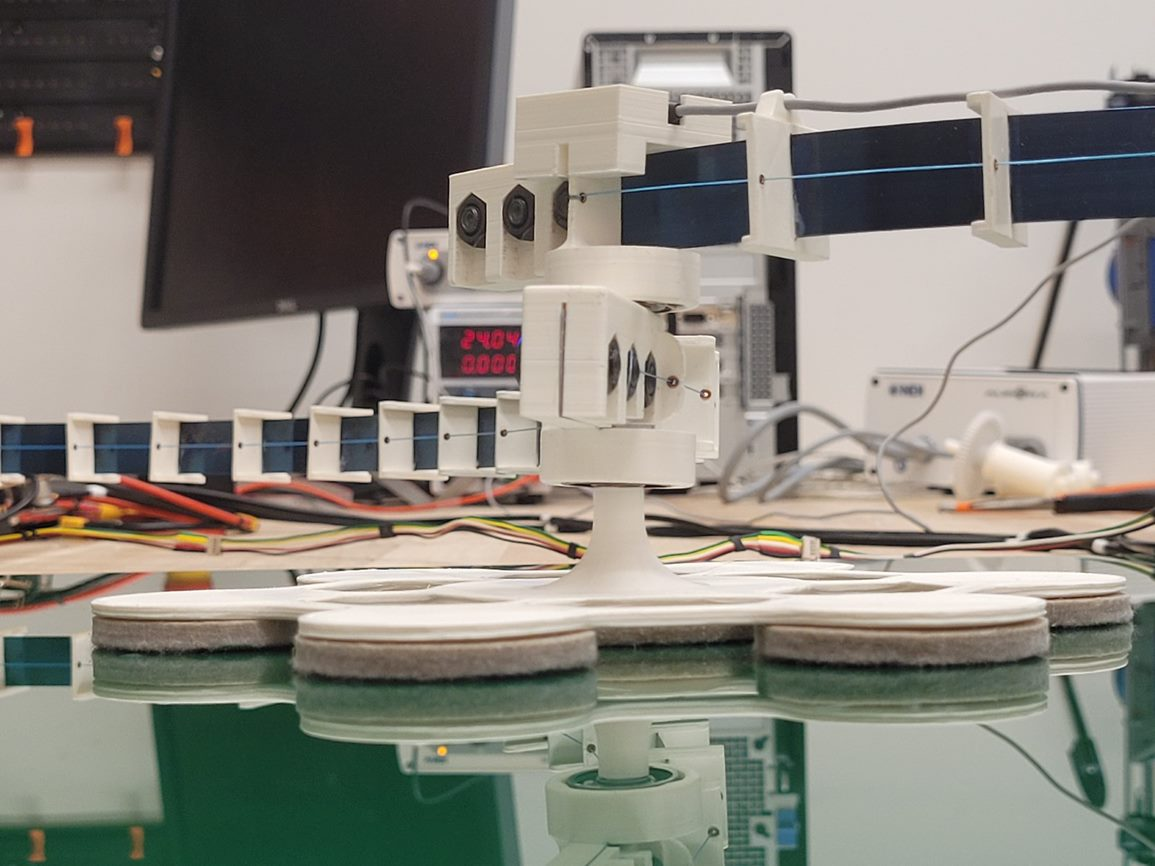
\includegraphics[width=\textwidth]{images/large_ee.jpeg}
         \caption{Larger base ensuring end effector remains on the plane}
         \label{fig:large_ee}
     \end{subfigure}
        \caption{Comparison of end effector sizes}
        \label{fig:ee_comparison}
\end{figure}

\paragraph{Gearboxes} are actuated directly by motors for each arm. The gear boxes are 3D printed but use purchase gears with a gear ratio of 16:1, enabling significantly higher applied torques than the motors are natively capable of. A 4:1 gear ratio is achieved by the motor unit. This results in a total gear ratio of 64:1 for the actuation unit. Each box contains two \SI{10}{mm} gears (2662N313, McMaster-Carr Supply Company, IL, USA) and three \SI{40}{mm} gears (2662N321, McMaster-Carr Supply Company, IL, USA) to achieve this rotation. The gearbox actuates a 3D printed spindle with a radius of \SI{11}{mm}. Two tendons are spooled around the spindle in opposite directions, so when it rotates, one tendon is extended while the other is contracted. Both tendons are firmly attached at the end effector side of each arm. This equal and opposite actuation of the tendons is what causes the arm to bend. 

% Workspace 
\paragraph{The workspace} additionally has an acrylic sheet used to reduce friction. Beneath the table surface, an AURORA electromagnetic tracking system (20-20 planar, Northern Digital Inc., ON, Canada) is positioned. The tracker is positioned to ensure maximal coverage of the robot's task space. The tracker is limited to an effective tracking area of \SI{50}{cm} x \SI{50}{cm} on the workspace plane. This unit tracks a wire coil which is fastened on the robot's end effector, directly above the revolute joint. This is where the end effector position is defined to be as a point in space. 

\subsubsection{Electronic Components}
Each arm is driven by a single Antigravity drone motor (MN4004 KV300, T-MOTOR, JX, P.R. China) which are both controlled by an off-the-shelf microprocessor (LAUNCHXL-F28069M, Texas Instruments, Dallas, USA) fitted with two booster cards (BOOSTXL-DRV8305EVM, Texas Instruments, Dallas, USA). The motors are part of an actuation unit shown in Figure \ref{fig:motor_unit} and contain a 4:1 gear ratio and an Avago optical encoder (AEDM 5810, Broadcom Inc., CA, USA) that is used to provide system feedback at a rate of \SI{1000}{hz} to the workstation. The actuation setup comes from the Open Continuum Robot project \cite{open_cr, Grimminger_2020}. A single micro-controller communicates with a workstation through the CAN bus protocol. The robot is powered using a \SI{240}{W} power supply operating at \SI{24}{V}. An emergency stop is installed within reach of the operator for safety. 

\begin{figure}[p]
    \centering
    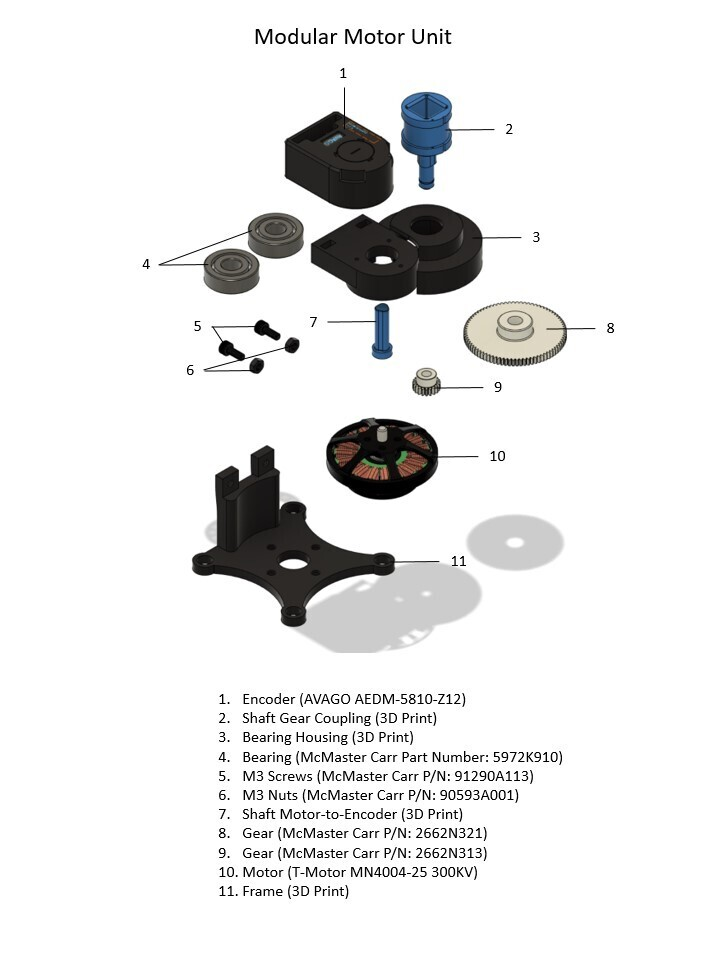
\includegraphics[width=\textwidth]{images/motor_unit.jpg}
    \caption{Complete schematic of the motor actuation unit, from \cite{motor_actuation_paper}}
    \label{fig:motor_unit}
\end{figure}

\paragraph{The workstation} used is a Dell OptiPlex 7090. It boasts an Intel Core i7-10700 CPU with 16GB of memory. It runs the RT-Preempt real time Linux kernel. The station communicates with the TI micro-controllers through a CAN-to-PCI Express interface card (IPEH-003027, PEAK system, Hessen, Germany). The station interfaces with the Aurora tracker through USB. Because the code for this thesis is written in Python, use of the real time kernel is not strictly required as Python does not support real time operations. For this project Python was deemed an appropriate language as it enables faster development times, and the shortcoming in terms of runtime is not seen to cause issues on the system. 

\subsubsection{Maximum Curvature Test}
Before the 16:1 gearbox was designed and installed, the actuation unit had a 4:1 gear ratio. An experiment was conducted to determine the arm length that enabled the largest range in the end effector position. Knowing the maximum and minimum distance that can be reached from an arm's base is required to set workspace bounds for the robot controller. The maximum distance is trivially given by the length of the arm. To find the minimum distance, a maximum curvature is applied by sending the highest current command a motor can support. The curvature that equates the bending forces to the maximum motor torque is taken as the maximum curvature. In this position, the distance between the end effector and arm base was measured. The results are displayed in Table \ref{tab:arm_length} and Figure \ref{fig:maximum_curve}. The arms were left at \SI{80}{cm} length as no notable gain in performance was observed at either test length. 

\begin{table}[h]
    \centering
    \caption{Arm distances during the maximum curvature test}
    \begin{tabular}{c|c|c}
        Extended Distance & Fully Contracted Distance & Contraction Distance \\
        \hline
        \SI{80}{cm} & \SI{59(1)}{cm} & \SI{21(1)}{cm} \\
        \SI{55}{cm} & \SI{33(1)}{cm} & \SI{22(1)}{cm} \\
    \end{tabular}
    \label{tab:arm_length}
\end{table}

This experiment showed the torque output of the motors resulted in a significantly smaller range of motion than what was initially expected. In response, a new gearbox was designed and manufactured to increase the maximum torque output of the robot. With the new gearbox, the robot is able to contract its arm completely with \SI{0}{cm} between the end effector and base. 

\begin{figure}[H]
     \centering
     \begin{subfigure}[b]{0.48\textwidth}
         \centering
         \includegraphics[width=\textwidth]{images/max_curve1.png}
         \caption{Without gearbox}
         \label{fig:maximum_curve1}
     \end{subfigure}
     \hfill
     \begin{subfigure}[b]{0.48\textwidth}
         \centering
         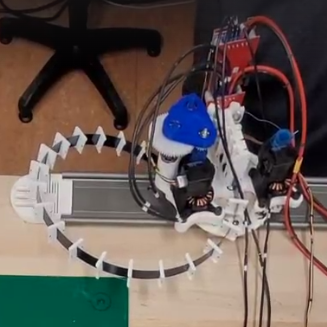
\includegraphics[width=\textwidth]{images/max_curve2.png}
         \caption{With gearbox}
         \label{fig:maximum_curve2}
     \end{subfigure}
        \caption{Maximum curvature tests}
        \label{fig:maximum_curve}
\end{figure}

 % Physical prototype 
\subsection{Robot System Controller}
The robot is controlled using the schematic shown in Figure \ref{fig:control_schematic}, referred to as the "system controller". This should not be confused with the "robot controller" which refers to the controller that maps target motions to joint values. 

\begin{figure}[h]
    \centering
    \makebox[\textwidth][c]{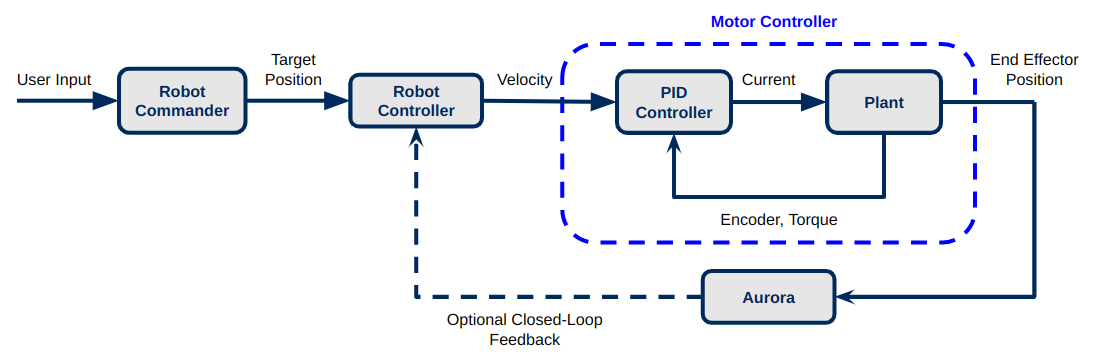
\includegraphics[width=\textwidth]{images/control_schematic.png}}
    \caption{Robot system controller schematic}
    \label{fig:control_schematic}
\end{figure}

\subsubsection{Controller Description}
\paragraph{A high level commander} module maintains the robot's state at all times. This module interfaces with the robot user, and determines which operation modes the robot is in. It handles logging, recovery behaviour, and manages a watchdog thread for each component of the system that will raise an error if any process dies. All robot states are described in Table \ref{tab:controller_states}. During states that are engaged in point tracking, a termination criteria of the end effector being within \SI{2}{cm} of the goal point is used. During trajectory tracking, no such condition is required as the goal point is progressed in time using a predefined trajectory. This module is referred to as the robot commander. 

\paragraph{A closed loop cascade controller} controls the motion of the robot. The inner loop uses a PID controller in conjunction with motor encoder feedback and a reference signal from the robot controller to determine the current to be sent to each motor. The gains used in this controller are shown in Table \ref{tab:motor_controller_gains}. This loop is referred to as the motor controller. 

\begin{table}[h]
    \centering
    \caption{Motor controller gains}
    \begin{tabular}{p{0.25\linewidth} | p{0.1\linewidth} | p{0.1\linewidth} | p{0.1\linewidth}}
        \textbf{Controller} & \textbf{$K_p$} & \textbf{$K_d$} & \textbf{$K_i$} \\
        \hline
        Position & 20 & 0.2 & 10 \\
        Position (Recovery) & 0.05 & 0.7 & 0.03 \\
        Velocity & 3 & 0 & 60 \\
    \end{tabular}
    \label{tab:motor_controller_gains}
\end{table}

\paragraph{The robot controller} determine the joint displacements or joint rates required to achieve a desired end effector motion. With this setup, the controller can either operate in a closed-loop scenario using measurements from the Aurora tracking system, or in an open-loop scenario, where an external state-estimation pipeline must be implemented. Explicit state estimation of this robot is outside of the scope of this thesis, so each proposed baseline controller will operate in the closed-loop configuration. 

\begin{table}[p]
    \centering
    \caption{Controller state description}
    \makebox[\textwidth][c]{\begin{tabular}{p{0.2\linewidth} | p{0.4\linewidth} | p{0.35\linewidth} }
        \textbf{State} & \textbf{Description} & \textbf{Exit Condition} \\
        \hline
        ERROR & The robot has experienced a critical error & Manual reset of the software and hardware \\
        \hline
        STOPPED & The robot is blocked from tracking reference signals. Used when the robot should remain stationary while code runs & State moves to READY after code is completed \\
        \hline
        RANDOM TRACKING & The robot is tracking random target points. Used during data collection & User terminated \\
        \hline
        REFERENCE TRACKING & The robot is tracking a pre-loaded reference trajectory. Used during model testing & Returns to READY when reference trajectory is complete  \\
        \hline
        REFERENCE STARTING & The robot is moving towards the start of a provided reference trajectory & Moves to HOLDING once the robot reaches the starting point to a reference trajectory \\
        \hline
        MANUAL TRACKING JOINT & The robot is tracking a point determined through the user control API in joint space & User terminated \\
        \hline
        MANUAL TRACKING TASK & The robot is tracking a point determined through the user control API in task space & User terminated \\
        \hline
        RECOVER & The robot is recovering from a lost Aurora signal. It is returning to the home position & Moves to READY when home position is reached \\
        \hline
        READY & The robot is stationary and able to take new commands & User terminated \\  \hline
        HOLDING & The robot is intentionally waiting at a point before progressing to the next command. Used during testing to provide time to set up video feeds & Moves to REFERENCE TRACKING after a set period of time \\
        \hline
    \end{tabular}}
    \label{tab:controller_states}
\end{table}

\subsubsection{Lost AURORA Recovery}
In the case of lost AURORA measurements, a recovery mode is entered where the robot returns to its home position using only motor encoder feedback. The home position is where both arms are fully extended and the motor encoders read a rotation of \SI{0}{rad}. This recovery behaviour is the only motion that can be executed in a closed-loop configuration without AURORA measurements.  % Control suite / state machine 
\subsection{Baseline Models}
\label{sec:baselines}
As no other research provides a baseline that can be compared to for this system, I propose two baseline controllers: a differential controller based on the constant curvature assumption and a PID controller based on a prismatic joint assumption. The selection of the constant curvature model is motivated by its ease of derivation and implementation. Other models, such as those based on a variable curvature backbone representation may provide more accurate results than our selected baseline at the expense of increased computation \cite{10.3389/frobt.2020.630245}. These models also have their own challenges representing the dynamic effects of continuum robots. Future works may look at the results of these models on this system but it is deemed as beyond the scope of this thesis. The PID controller was chosen as it is a fast model both in runtime and implementation time, and can be tuned to work reasonably well in a closed-loop scenario.  

\subsubsection{Robot Model}
First, a robot model is developed that maps an arm's curvature value to a tendon displacement. Equation \eqref{eq:ik_ktoq} solves for the change of tendon length required to achieve a given constant curvature. Two solutions are provided, one for each side of the beam. Equation \eqref{eq:ik_ktoq} is used to find the tendon length given a beam's curvature, assuming a fully constrained tendon path \cite{10.3389/frobt.2020.630245} along the length of the beam. 

\begin{equation}\label{eq:ik_ktoq}
    \Delta l_{t,i} = \pm\ell_i\ell_t\kappa_i
\end{equation}

Equation \eqref{eq:ik_ktoq} can be extended to consider the prototype motor's gear ratio and spindle radius which the tendons are wrapped around. This gives an expression for the motor rotation required to achieve the desired tendon length displacement. The motor rotation $q$ found in Equation \eqref{eq:joint} is the joint variable for the proposed PCR. I take the positive solution as both tendons are actuated in their respective directions by the same motor. 

% Joint variable calculation 
\begin{equation}\label{eq:joint}
    q = \kappa G \ell_i \frac{\ell_t}{r_m}
\end{equation}

\subsubsection{Constant Curvature Controller}
A model using the constant curvature assumption \cite{doi:10.1177/0278364910368147} is used as a baseline model for this parallel continuum robot. This model is used to solve the inverse kinematic problem. This is used to determine control signals for the robot during the data generation, enabling the ability to control the position of the end effector (with some error). Equation \eqref{eq:cc/ik} gives a general expression relating the curvature of a constant curvature beam and a beam's base and end position \cite{slilge_2020}. 

\begin{figure}[H]
    \centering
    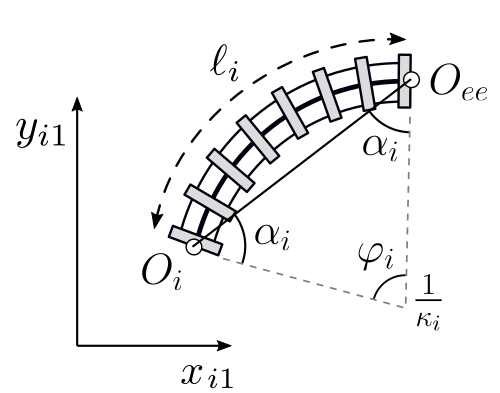
\includegraphics[width=0.6\textwidth]{images/constant_curvature_link.png}
    \caption{Constant curvature model diagram}
    \label{fig:cc_controller}
\end{figure}

% Inverse Kinematic Equation
\begin{align*}
|| O_{ee} - O_i || &= 2\frac{1}{\kappa_i}\cos(\alpha_i) \\
&= 2\frac{1}{\kappa_i}\sin\left(\frac{\varphi_i}{2}\right)\\
h(\kappa_i, O_{ee}) = h_i = 0 &= \frac{2}{\ell_i\kappa_i} \sin\left(\frac{\ell_i\kappa_i}{2}\right) - \frac{|| O_{ee} - O_i ||}{\ell_i}\stepcounter{equation}\tag{\theequation}\label{eq:cc/ik}
\end{align*}

The solution for $\kappa$ is found by finding the roots of Equation \eqref{eq:cc/ik}. For the parallel continuum case, one solves Equation \eqref{eq:cc/ik} for each of the robot's arms. One extra check is required that the target point is within reach of each arm to guarantee a solution. The solution is found numerically using scipy.optim.fsolve\footnote{\url{https://github.com/scipy/scipy/blob/v1.10.0/scipy/optimize/_minpack_py.py\#L48-L181}}. As this model is strictly a position controller, it does not have the ability to reduce the robot's steady state error between its end effector and a goal point to zero. As such, I do not explore this controller in depth on the system, but rather use it as a starting point for its differential counterpart. 

\subsubsection{Differential Constant Curvature Controller}
By taking the derivative of Equation \eqref{eq:cc/ik} with respect to time, we can derive a differential version of the constant curvature position controller. This enables us to control the robot using velocity control in the motor controller. 

\begin{equation*}\label{eq:cc_diff/intial}
    \frac{\partial h}{\partial \kappa}\frac{\partial \kappa}{\partial t} + \frac{\partial h}{\partial O_{ee}}\frac{\partial O_{ee}}{\partial t} = 0
\end{equation*}

\begin{equation*}\label{eq:cc_diff/matrices}
    A = \begin{bmatrix}
        \displaystyle\frac{\partial h_1}{\partial \kappa_1} & 0\\
        0 & \displaystyle\frac{\partial h_2}{\partial \kappa_2} \\
        \end{bmatrix}, 
    B = \begin{bmatrix}
        \displaystyle\frac{\partial h_1}{\partial O_{ee, x}} & \displaystyle\frac{\partial h_2}{\partial O_{ee, y}}\\
        \displaystyle\frac{\partial h_1}{\partial O_{ee, x}} & \displaystyle\frac{\partial h_2}{\partial O_{ee, y}} \\
        \end{bmatrix}
\end{equation*}

\begin{equation*}
    A \dot \kappa + B \dot O_{ee} = 0 
\end{equation*}

While matrices A and B are invertible, they contain the $\kappa_i$ terms which must still be found numerically. A closed form solution to this model does not exist. 

\begin{equation}\label{eq:cc_diff/ik}
    \mathbf{\dot{\kappa}} = (-B^{-1}_iA_i)^{-1}\dot{O_{ee}} 
\end{equation}

In this particular model, point tracking is achieved by defining an error term between the end effector position and the goal point, and using a simple P controller to determine the desired end effector velocity. A value of $K_p = 0.01$ is used. This is shown in Equation \eqref{eq:cc_diff/gain} and can be combined with Equation \eqref{eq:cc_diff/ik} to retrieve the full controller model for the differential constant curvature controller shown in Equation \eqref{eq:cc_diff/gain_ik}. 

\begin{equation}\label{eq:cc_diff/gain}
     \dot O_{ee} = K_p|| O_{goal} - O_{ee} ||
\end{equation}
\begin{equation}\label{eq:cc_diff/gain_ik}
     \mathbf{\dot{\kappa}} = K_p(-B^{-1}_iA_i)^{-1} || O_{goal} - O_{ee} ||
\end{equation}

Using the robot model from Equation \eqref{eq:joint} yields the complete differential constant curvature controller shown in Equation \eqref{eq:cc_diff/complete}. $\dot q$ can be commanded directly to the motor controller as a velocity set point. 

\begin{equation}\label{eq:cc_diff/complete}
     \dot q = K_pG \ell_i \frac{\ell_t}{r_m}(-B^{-1}_iA_i)^{-1} || O_{goal} - O_{ee} ||
\end{equation}

\subsubsection{Prismatic Assumption PID Controller}

A second controller is proposed by modelling each continuum arm as a prismatic joint. The idea is that the arm is capable of contracting and extending, which simply actuates the distance between the end effector and an arm's base point. Because the robot's workspace is clear of obstacles, no concern is required for maintaining an estimate of the shape of the robot. For every goal point, each arm has a specific distance it needs to extend or contract to which can be solved for independently of the other arms. 

\begin{figure}[H]
    \centering
    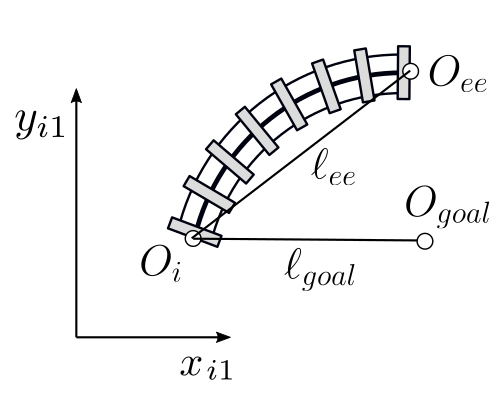
\includegraphics[width=0.6\textwidth]{images/pid_controller.png}
    \caption{Prismatic PID model diagram}
    \label{fig:pid_controller}
\end{figure}

An error term (Equation \eqref{eq:pid/error}) is defined by subtracting the distance between the goal point and an arm's base, and the end effector position and an arm's base. This error is used in a PID controller to yield the joint velocity command in Equation \eqref{eq:pid/complete}. The gains found to result in desirable behaviour are $K_p = 4, K_d = 0, K_i = 0$. 

\begin{align}
    e_i(t) &= ||O_{goal} - O_i|| - ||O_{ee} - O_i|| \label{eq:pid/error}\\
        &= \ell_{goal} - \ell_{ee} \nonumber\\
    \dot q_i &= K_pe_i(t) + K_d \frac{de_i}{dt} + \int e_i(t)dt\label{eq:pid/complete}
\end{align}

This controller has a closed form update, suggesting a computational advantage over the differential constant curvature model which must be solved iteratively. It also is significantly easier to derive and implement in software, making it a fast and easy option for controlling this robot. Because the model does not solve for a curvature value, the robot model is not required. The conversion to motor velocities is handled in the controller gains.  % Baseline models 
\subsection{Data Collection}
\label{sec:data_methods}

\subsubsection{Workspace Coordinate Frame Definition}
The workplace has a coordinate frame defined by three point markings on the green acrylic sheet at three corners (shown in Figure \ref{fig:workspace}). During regular operation of the robot, all readings from the AURORA system are transformed to be represented in the workspace coordinate frame (sometimes referred to as the "robot frame"). A method is used to calibrate the reference frame between each session on the robot. A total of 30 AURORA measurements are taken at each of the three points. The average position of the points is found by a simple mean over the 30 readings. The origin of the workspace is taken to be the location of the first point, $O_1$. The workspace axes are defined as follows: 

\begin{align*}
    \hat{x} &= \frac{O_3 - O_1}{||O_3 - O_1||} \\
    \tilde{y} &= \frac{O_2 - O_1}{||O_3 - O_1||} \\
    \hat{z} &= \hat{x}\times\tilde{y} \\
    \hat{y} &= \hat{z}\times\hat{x}
\end{align*}

\begin{figure}[h]
    \centering
    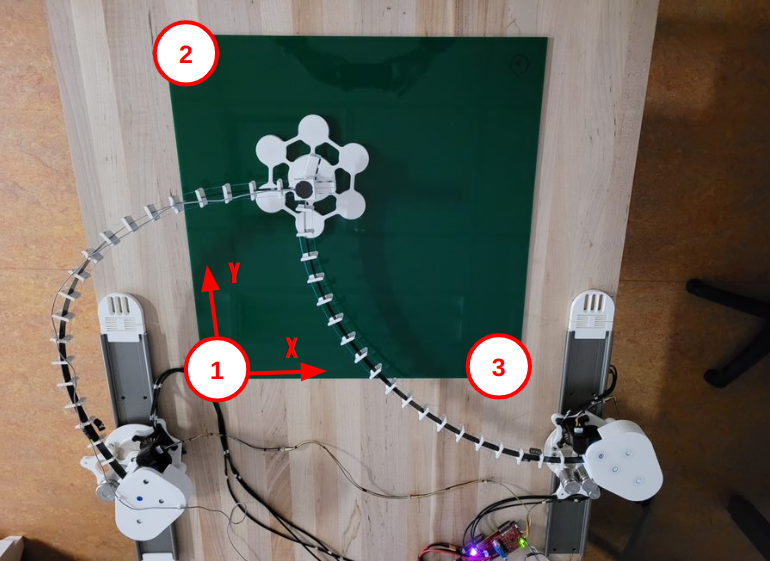
\includegraphics[width=0.8\textwidth]{images/workspace.png}
    \caption{Robot workspace coordinate frame diagram}
    \label{fig:workspace}
\end{figure}


\subsubsection{Data Schema}
Data is collected from all parts of the system at various rates as described in Table \ref{tab:data_schema}. All data during operation is saved to log files with unique names that can later be loaded into a dataloader object. 

\begin{table}[h]
    \centering   
    \caption{Robot data collection schema}
    \begin{tabular}{p{0.5\linewidth} | p{0.15\linewidth} | p{0.2\linewidth}}
        \textbf{Data Type} & \textbf{Unit} & \textbf{Frequency in Hz} \\
        \hline
        \multicolumn{3}{c}{Motor Controller} \\
        \hline
        Current command & A & 100 \\
        Current draw & A & 100 \\
        Motor position set point & rad & 100 \\
        Motor position & rad & 100 \\
        Motor angular velocity set point & rad/s & 100 \\
        Motor angular velocity & rad/s & 100 \\
        Controller type & N/A & 100 \\
        Recording timestamp & s & 100 \\
        \hline
        \multicolumn{3}{c}{AURORA System} \\
        \hline
        End effector position (AURORA frame) & m & 5 \\
        End effector orientation (AURORA frame) & m & 5 \\
        End effector position (robot frame) & m & 5 \\
        Recording timestamp & s & 5 \\
        \hline
        \multicolumn{3}{c}{Robot Commander} \\
        \hline
        Sample termination cause & From table \ref{tab:termination_types} & On termination \\
        Commander state & From table \ref{tab:controller_states} & 5 \\
        Recording timestamp & s & 5 \\
        \hline
    \end{tabular}
    \label{tab:data_schema}
\end{table}


\subsubsection{Collection Method}
\paragraph{The robot controller} used for data collection is the prismatic assumption PID baseline controller from Equation \eqref{eq:pid/complete}. It was selected because of its good relative performance on a number of metrics discussed in Section \ref{sec:baseline_comparison}. Data was only collected using this single baseline due to project timing limitations. As such, the data collected only contains robot states that are accessible using this controller, which has the potential to instill bias into the dataset. 

\paragraph{The sampling method} used for deciding which paths to move the robot over is a random sampling over a uniform distribution. Sample goal points are drawn inside a \SI{15}{cm} radius of the end effector position at the start of the sample and outside a \SI{5}{cm} radius of that same position. An upper bound of \SI{15}{cm} was selected as much above that would result in harsh robot movements that caused damage to the robot. A lower bound of \SI{5}{cm} was selected as much below that would result in motor set points that result in an applied motor torque that is too low to overcome the static friction of the end effector in some positions in the workspace. 

A more complex path sampler was explored using randomized path generation while ensuring joint actuation smoothness, but was ultimately removed as it did not satisfy the workstation's real time runtime constraints. More information on this method is presented in Appendix \ref{app:path_planner}. 


\subsubsection{Termination Cases}
\paragraph{Non-critical failures} occur when for some reason the robot is not able to find a way to withing a \SI{2}{cm} radius of the sampled goal point. A number of reasons can cause this, including lost AURORA measurements or a stalled end effector. The robot can recovery without user intervention from non-critical failure cases and the data from them is complete and usable. 

\paragraph{Critical failures} occur when the robot failed in a way that could result in corrupted data. This happens when a portion of the code crashes or the robot loses power, typically by the user hitting the emergency stop. In critical failure cases the user must reset the system manually and delete the affected data logs. 

\paragraph{Successful samples} occur when the robot successfully arrives at the sampled goal point without triggering any of the failure cases. A full description of all termination causes is provided in Table \ref{tab:termination_types}. 

\begin{table}[h]
    \centering   
    \caption{Robot sample termination types}
    \begin{tabular}{p{0.3\linewidth} | p{0.6\linewidth}}
        \textbf{Termination Type} & \textbf{Description} \\
        \hline
        Success & The robot successfully reached the target point \\\hline
        Stalled & The robot's end effector velocity was below \SI{0.001}{m/s} for more than \SI{5}{s} \\\hline
        Aurora lost & At least 3 consecutive AURORA measurements were errors, typically caused by the end effector leaving the workspace \\\hline
        Recovery & The robot underwent recovery behaviour where AURORA readings are not necessarily available \\\hline
        Mode switch & The robot operator manually switched the robot into a different mode \\\hline
        User terminated & The user shut down the system using the control interface \\\hline
        Tracking finished & A reference trajectory was completed \\\hline
        Error & An error is raised during the trial. This results from a crashed thread, or a failed recovery attempt \\\hline

    \end{tabular}
    \label{tab:termination_types}
\end{table} % Data Collection 
\subsection{Learning Pipeline}
Two primary learning-based control pipelines are supported by this project. The first has trained models replacing both the robot controller and motor controller in the robot system. These models take as inputs a target position with system feedback and directly outputs motor current commands. The second has a trained model that acts as the robot controller, leaving the motor control loop as is.  

\begin{figure}[H]
     \centering
     \begin{subfigure}[b]{\textwidth}
         \centering
         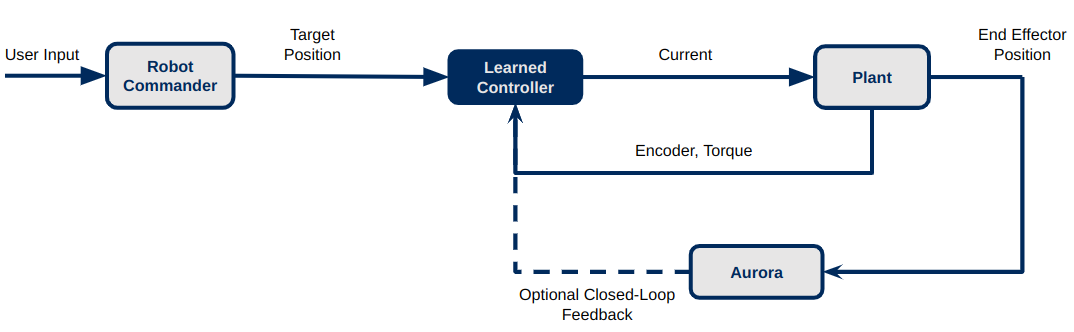
\includegraphics[width=0.9\textwidth]{images/learned_option1.png}
         \caption{Learning-based controller implementation replacing motor controller}
         \label{fig:learning_model1}
     \end{subfigure}
     \hfill
     \begin{subfigure}[b]{\textwidth}
         \centering
         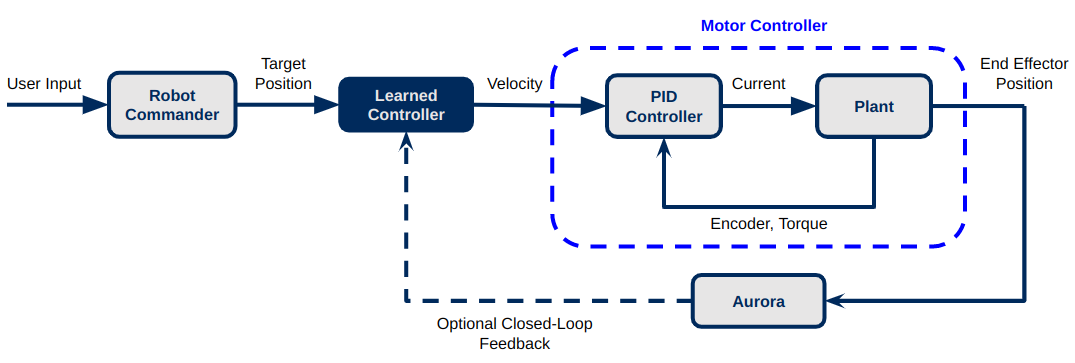
\includegraphics[width=0.9\textwidth]{images/learned_option2.png}
         \caption{Learning-based controller implementation as just the robot controller}
         \label{fig:learning_model2}
     \end{subfigure}
        \caption{Learning-based controller implementation pipeline options}
        \label{fig:learning_model_options}
\end{figure}

\paragraph{Option 1} 
In the first option (Figure \ref{fig:learning_model1}), the learned model is responsible for more aspects of control. This gives the model more flexibility in its approach to control as it has access to a lower-level control signal. However, elements of control that the PID motor controller accounts for such as limiting the change in command signals or reducing accumulated error over time are also required to be learned to achieve comparable performance. 

\paragraph{Option 2}
In the second option (Figure \ref{fig:learning_model2}), the motor controller remains in the loop. This approach has the learned controller replace one of the two baseline controllers presented in Section \ref{sec:baselines}.  This approach may be limited in accuracy as the inclusion of a PID controller restricts the system's output. 

\subsubsection{Dataloaders}
Two dataloaders were developed in order to provide an interface between the robot's data logs and the Pytorch deep learning library\footnote{https://pytorch.org/}, one designed for learning control and the other for state estimation.

\begin{figure}[H]
     \centering
     \begin{subfigure}[b]{0.8\textwidth}
         \centering
         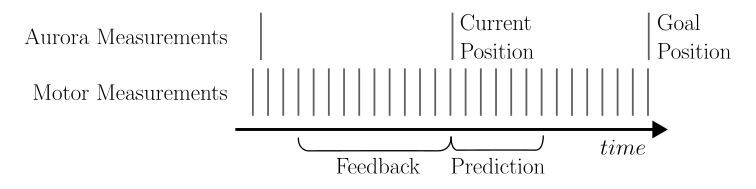
\includegraphics[width=\textwidth]{images/dataloader1.png}
         \caption{Control dataloader data representation}
         \label{fig:dataloader1}
     \end{subfigure}
     \hfill
     \begin{subfigure}[b]{0.8\textwidth}
         \centering
         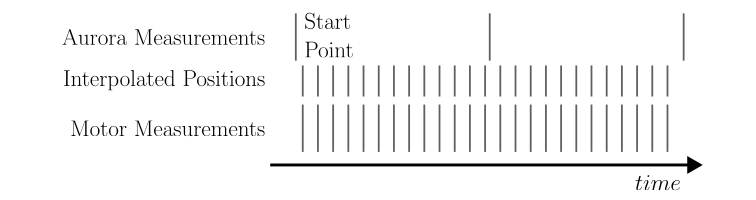
\includegraphics[width=\textwidth]{images/dataloader2.png}
         \caption{State estimation dataloader data representation}
         \label{fig:dataloader2}
     \end{subfigure}
        \caption{Representation of data loader with dataloader}
        \label{fig:dataloaders}
\end{figure}

\paragraph{The control dataloader} provides as input the robot's current ground truth position, a horizon of feedback from the motor controller, and the robot's next ground truth position. Each of these inputs is available to the robot in real time during closed-loop operation. For open-loop control, the current position input should either not be used or replaced with the output of a state estimation module. The labels provided are the next N motor commands. Figure \ref{fig:dataloader1} shows the timing breakdown of each of the provided pieces of data for this dataloader. 

\paragraph{The state estimation dataloader} provides as input the robot's starting position, and a series of feedback from the motor controller. The labels provided are an interpolation of the robot's ground truth state as measured at each motor controller feedback tick. The dataloader linearly interpolates the AURORA data to provide a state vector for every motor feedback command available. Figure \ref{fig:dataloader2} shows the timing breakdown of each of the provided pieces of data for this dataloader. 
 % Learning pipeline
\subsection{Learning Experiments}

\subsubsection{Model Architecture}

A base model architecture is used as a starting point for all learning experiments and is shown in Figure \ref{fig:architecture}. It consists of a head, a backbone, and a state estimator. The head consists of a configurable set of linear layers using the ReLU activation function. The backbone similarly is a configurable set of linear layers using the ReLU activation function that take as input the starting and goal position, along with any configuration parameters for the given dataset. These configuration parameters are tunable values that are indexed based on which robot setup was used to collect that data. A new configuration parameter is used for each time the robot has its tendons replaced. The state estimator is a configurable set of LSTM cells that take as input a horizon of motor feedback data. Specifically, experiments use current draw, encoder position, and encoder velocity for each motor. The output of the head is passed to one last linear layer without an activation layer. The output is then reshaped to be an $N\times 2$ vector where $N$ is the prediction horizon of the model. 

\begin{figure}[h]
    \centering
    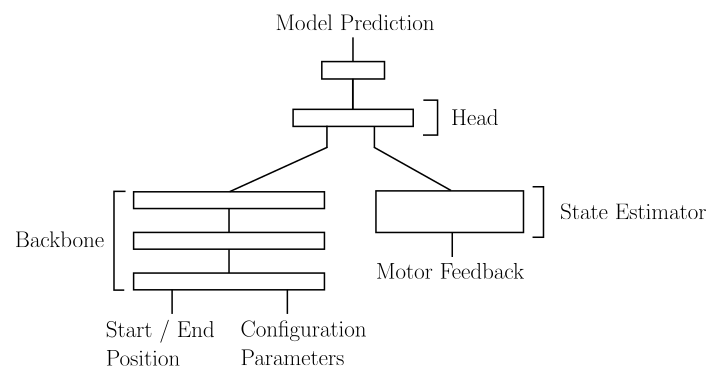
\includegraphics[width=0.8\textwidth]{images/architecture.png}
    \caption{Base model architecture for learning-experiments}
    \label{fig:architecture}
\end{figure}


\subsubsection{Training Parameters}
\label{sec:learning_baseline_description}
\paragraph{RMSE loss} is used for both training and comparing validation performance on a holdout dataset for each experiment (Equation \eqref{eq:rmse}). 

% Joint variable calculation 
\begin{equation}\label{eq:rmse}
    \operatorname{RMSE} = \sqrt{\frac{\displaystyle\sum_{i=1}^{N} ||y_{pred} - y_{gt}||^2 }{N}}
\end{equation}
where:
\begin{conditions}
y_\text{pred} & Predicted label from learned model \\
y_\text{gt} & Dataset label  \\
N & Number of items predicted \\
\end{conditions}

\paragraph{Constant training parameters} described in Table \ref{tab:training_parameters} are set and remained constant between all experiments. A runtime rate of \SI{1000}{Hz} for individual model calls is enforced for each trial to ensure that any model trained is capable of running in real time on the robot.  

\paragraph{Variable training parameters} described in Table \ref{tab:training_parameters} are varied through a series of experiments to find the optimal values for reducing validation loss. In each of these experiments (omitting the model architecture search trials), a baseline configuration is used as a comparison.

\begin{table}[h]
    \centering   
    \caption{Training parameters for learning experiments}
    \begin{tabular}{p{0.45\linewidth} | p{0.2\linewidth}}
        \textbf{Parameter} & \textbf{Value} \\
        \hline
        \multicolumn{2}{c}{Static Parameters} \\
        \hline
        Optimizer & Adam (default parameters) \\
        Learning rate & 0.001 \\
        Batch size & 512 \\
        Epochs & 1000 \\
        Early stopping & 10 \\
        \hline
        \multicolumn{2}{c}{Variable Parameters} \\
        \hline
        Feedback horizon & 1 - 300 \\
        Backbone layers & 1 - 3 \\
        Backbone layer size & 10 - 30 \\
        Head layers & 0 - 3 \\
        Head layer size & 0 - 50 \\
        LSTM layer size & 0 - 40 \\
        Configuration parameter size & 0 - 20 \\
        Data weights & Multiple \newline functions \\ 
    \end{tabular}
    \label{tab:training_parameters}
\end{table}

 % Learning experiments
\pagebreak
\section{Results}
\label{sec:results}
\subsection{Prototype Hardware}
% Add drawings / design philosophy 
The robot is designed with the Open Continuum Robotics project in mind. It uses easily accessible, off-the-shelf components, and 3D printed parts so that other groups can reconstruct the same robot. A full breakdown of the robot's physical design can be found in Appendix \ref{app:robot_drawings}. 

\subsubsection{Physical Description of Prototype}
\label{sec:physical_description}
% Arms
\paragraph{The arms} are each \SI{80}{cm} long and consist of a \SI{0.0200}{"} thick, \SI{0.75}{"} wide beam made from 1095 spring steel, with 19 evenly spaced 3D printed tendon spacers. The spacers hold one tendon on each side of the beam \SI{11}{mm} away from the steel beam. The 1095 spring steel beam is used as the central beam as it provides rigidity in the direction of motion off the robot's planar surface, while remaining flexible along the plane. The high elasticity of the material allows the system to undergo large curvatures without permanently deforming the beam. The tendons used are \SI{30}{lbs} braided fishing line (Super8Slick V2, Power Pro, CA, USA). Each tendon has four \SI{0.75}{"} nuts on it that act to maintain tension during operational periods where it is being extended. 

\begin{figure}[h]
    \centering
    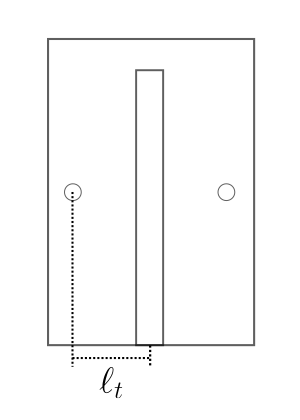
\includegraphics[width=0.3\textwidth]{images/beam_cross_section.png}
    \caption{Cross section of the beam spacers. $\ell_t = \SI{11}{mm}$}
    \label{fig:beam_cross_section}
\end{figure}

\begin{figure}[h]
    \centering
    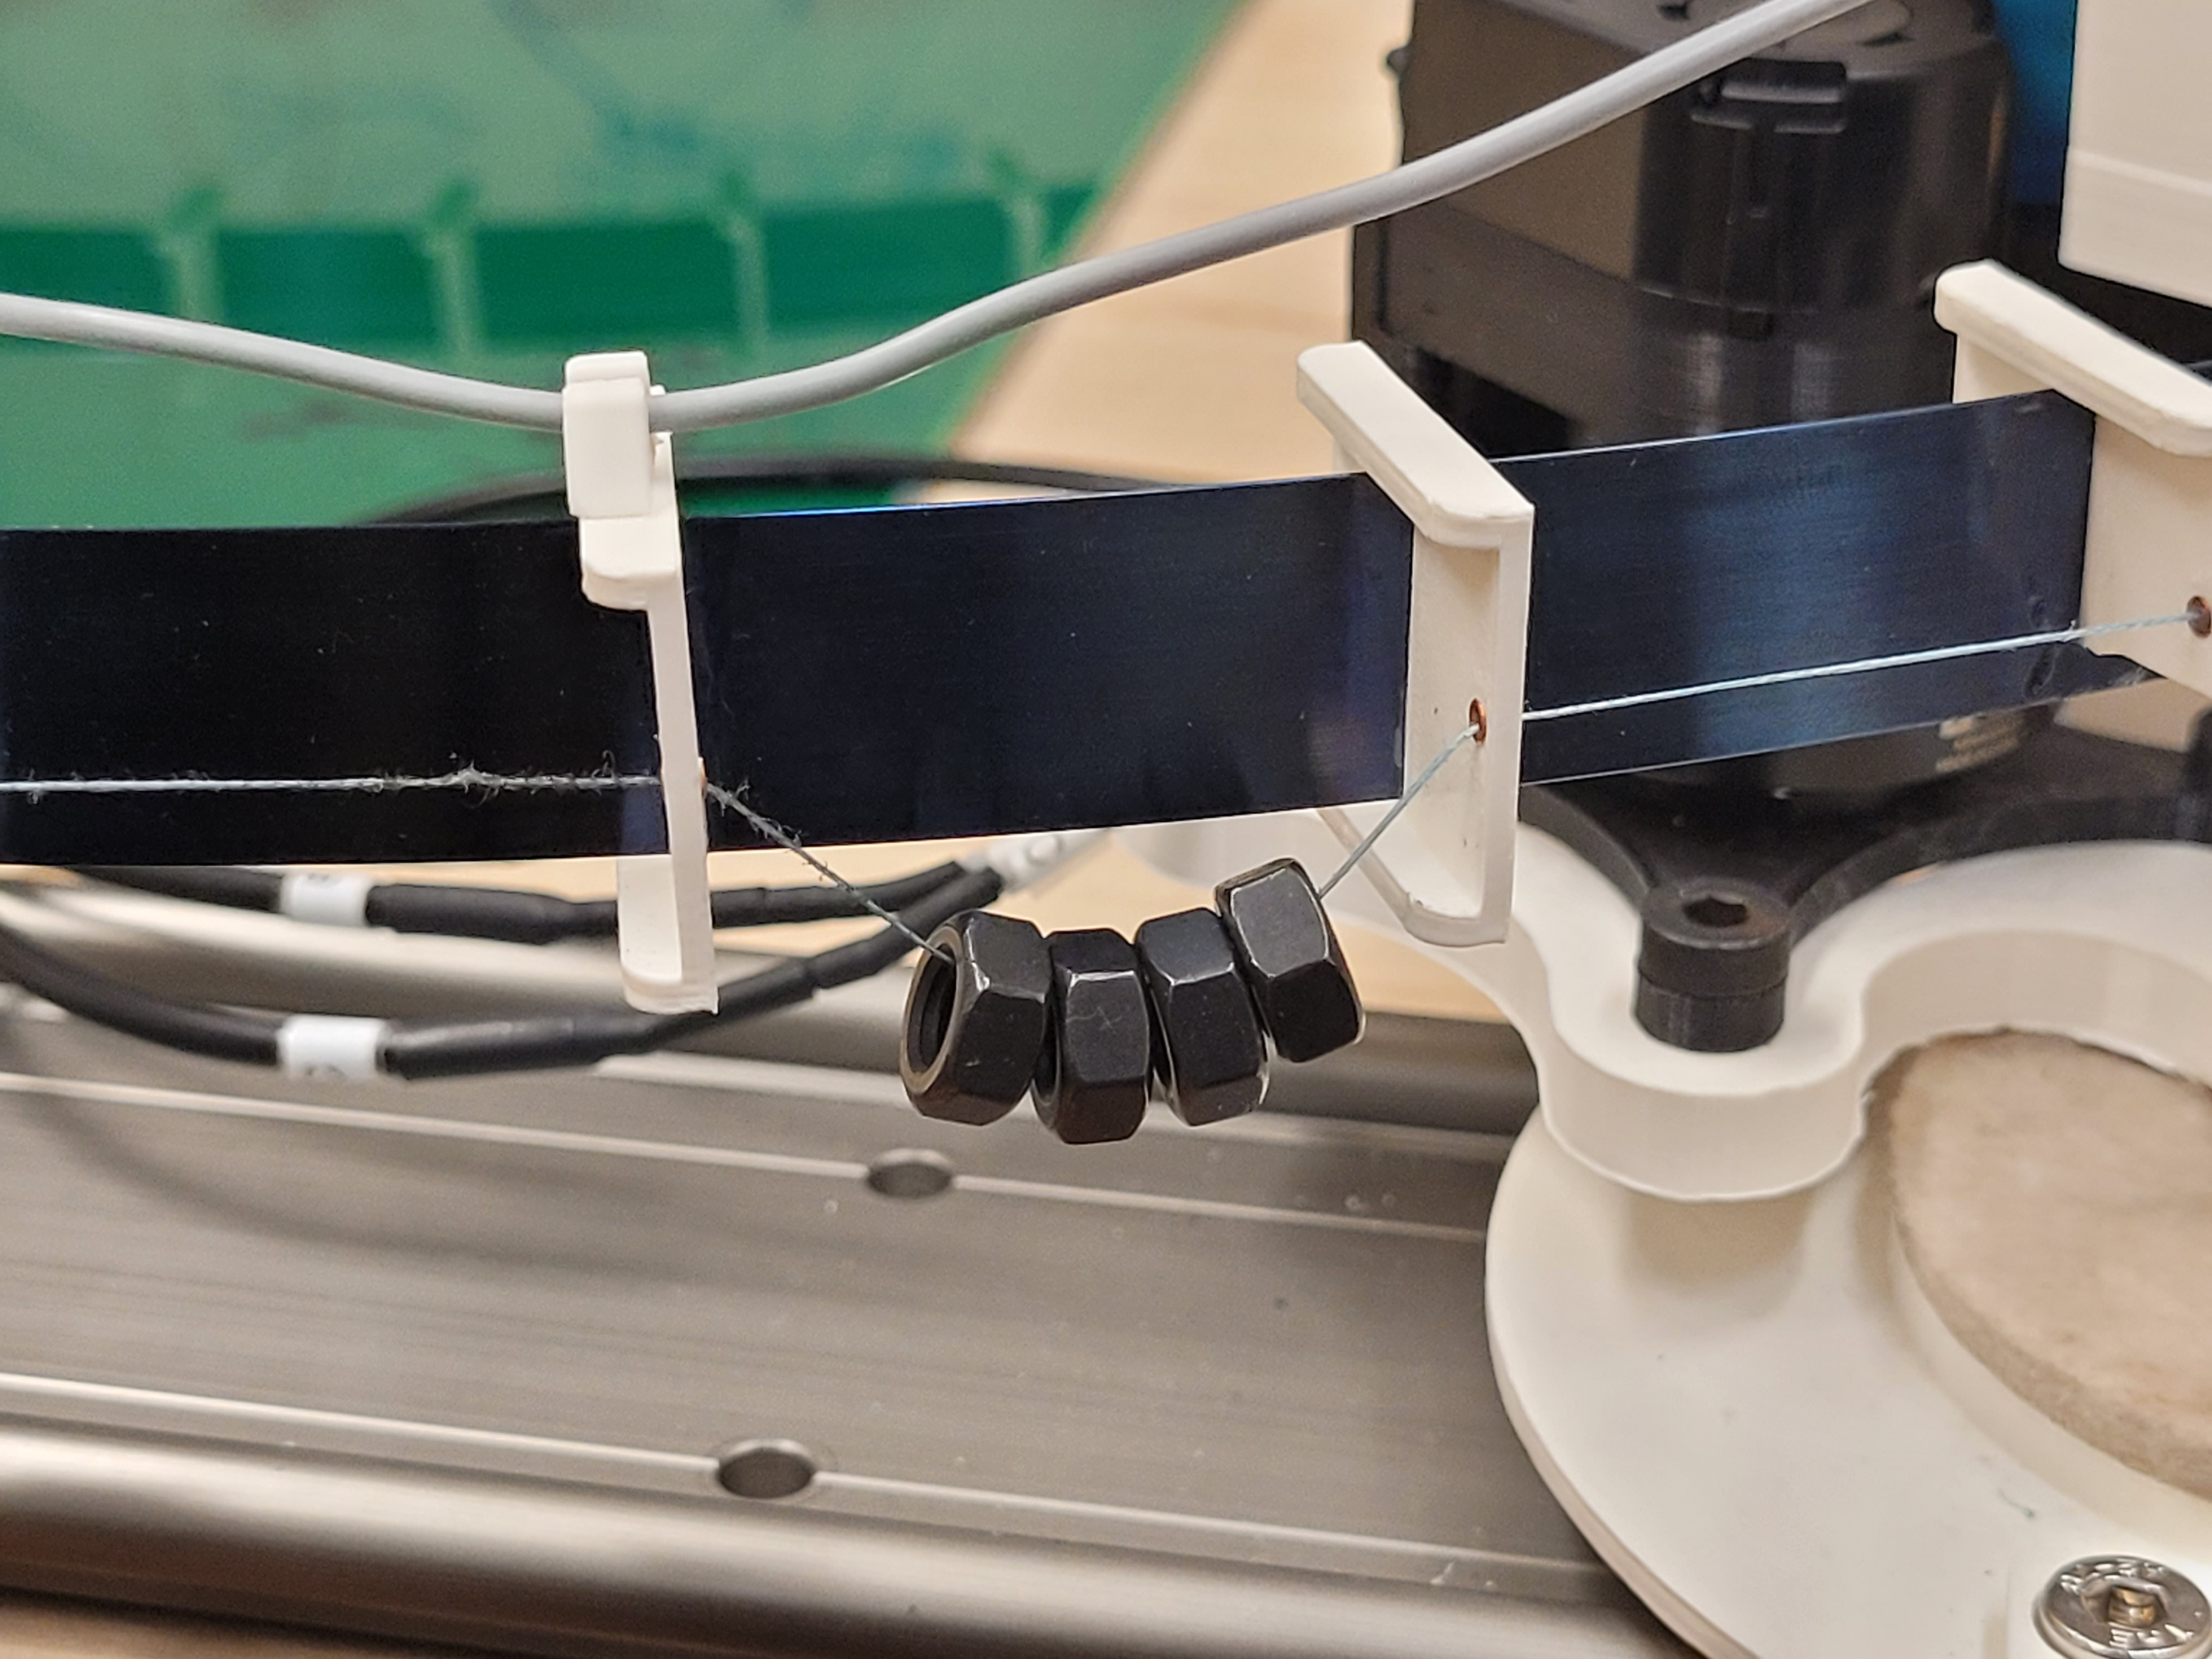
\includegraphics[width=0.5\textwidth]{images/tendon_slack.jpg}
    \caption{Four \SI{0.75}{"} nuts placed on a tendon to maintain tendon tension throughout operation}
    \label{fig:tendon_slack}
\end{figure}

% \begin{figure}[h]
%      \centering
%      \begin{subfigure}[b]{0.48\textwidth}
%          \centering
%          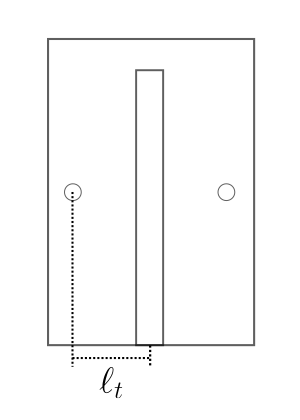
\includegraphics[width=0.625\textwidth]{images/beam_cross_section.png}
%          \caption{Cross section of the beam spacers. $\ell_t = \SI{11}{mm}$}
%          \label{fig:beam_cross_section}
%      \end{subfigure}
%      \hfill
%      \begin{subfigure}[b]{0.48\textwidth}
%          \centering
%          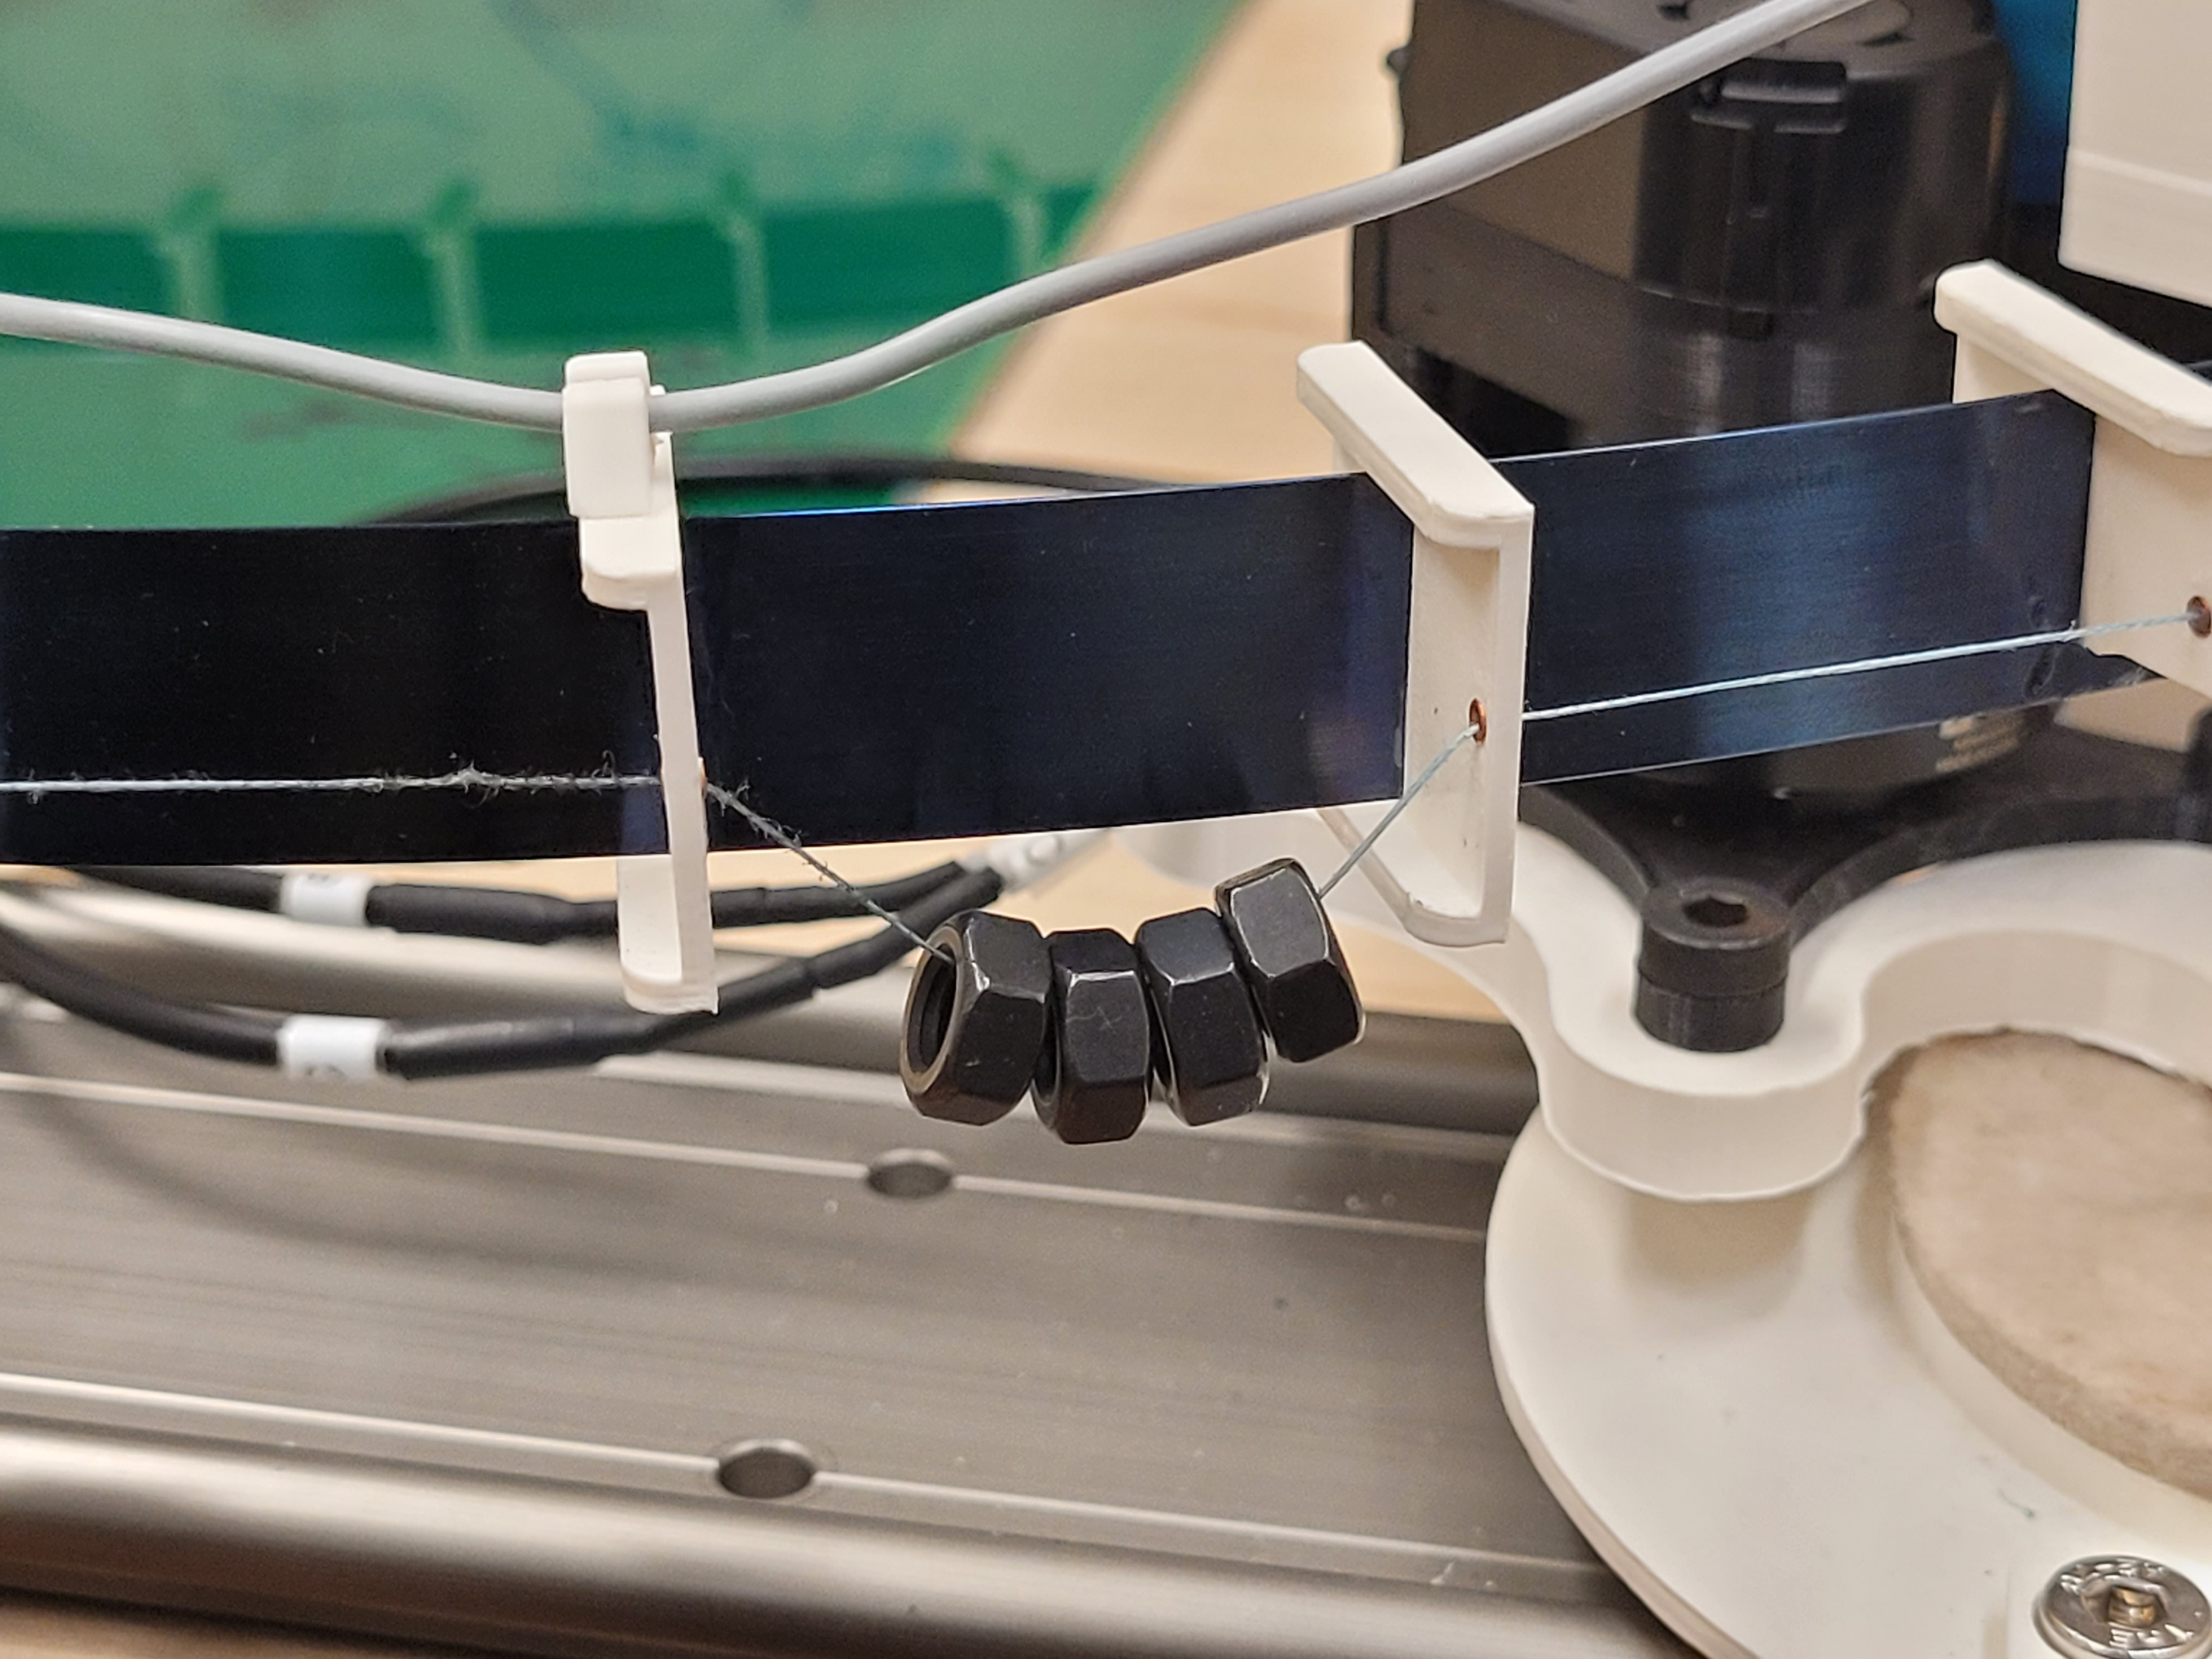
\includegraphics[width=\textwidth]{images/tendon_slack.jpg}
%          \caption{Four \SI{0.75}{"} nuts placed on a tendon to maintain tendon tension throughout operation}
%          \label{fig:tendon_slack}
%      \end{subfigure}
% \end{figure}

% Joints and End Effector  
\paragraph{The end effector} features a wide base to prevent the end effector from twisting off the plane. Revolute joints link the ends of each arm to the motor bases and the end effector, allowing both ends to rotate freely about the z-axis. The two arms share the same end effector. The bases for each arm are positioned \SI{60}{cm} apart.Each arm having its own independent degree of freedom grants the end effector in this configuration two degrees of freedom laying on the table plane. At this distance, the reachable workspace of the end effector covers a majority of the AURORA tracker workspace. During operation, a smaller end effector base does not provide enough area to balance the moments being applied by the two arms actuating the piece from different heights. Figure \ref{fig:ee_comparison} demonstrates this effect in action. Felt pads are attached to the bottom of the end effector to reduce friction between the end effector and table surface. 

\begin{figure}[h]
     \centering
     \begin{subfigure}[b]{0.48\textwidth}
         \centering
         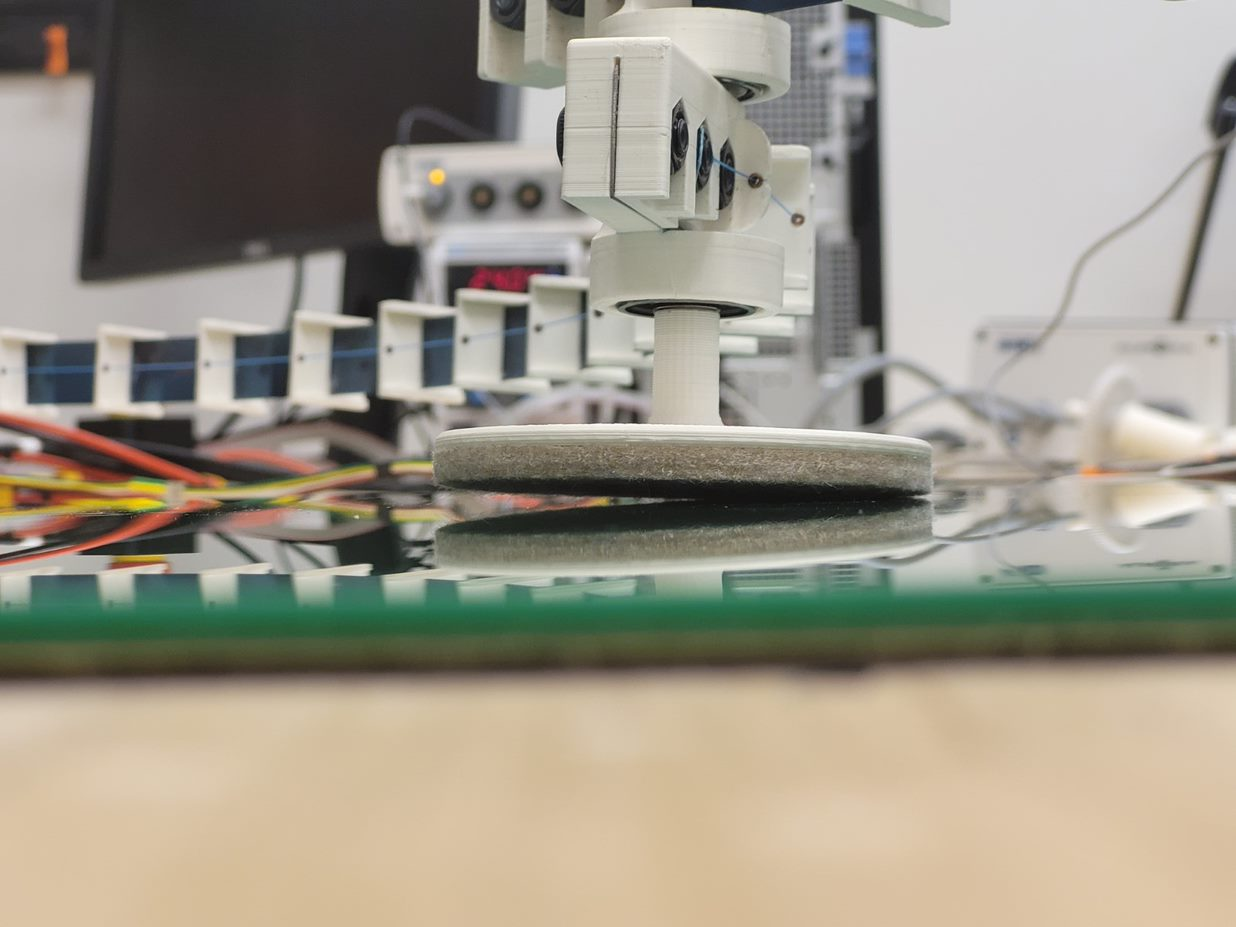
\includegraphics[width=\textwidth]{images/small_ee.jpeg}
         \caption{Smaller base causing the end effector to twist off the planar surface}
         \label{fig:small_ee}
     \end{subfigure}
     \hfill
     \begin{subfigure}[b]{0.48\textwidth}
         \centering
         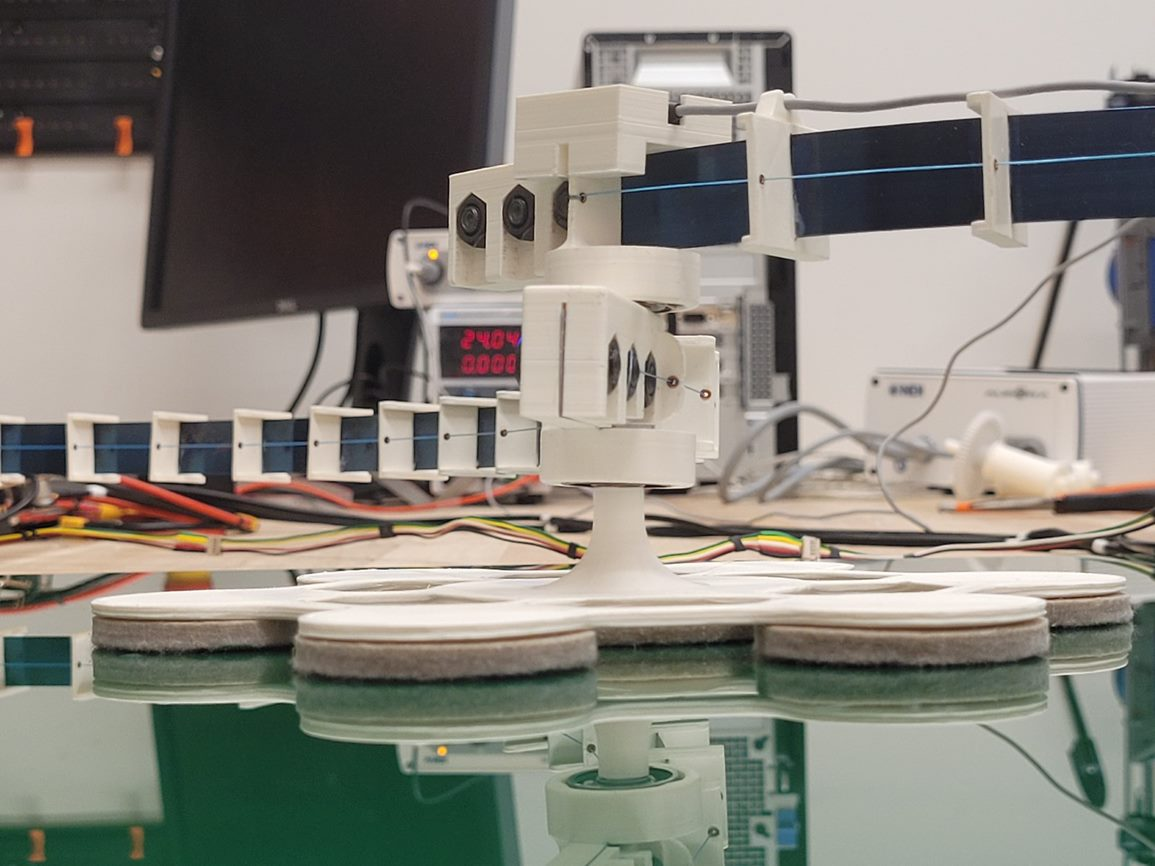
\includegraphics[width=\textwidth]{images/large_ee.jpeg}
         \caption{Larger base ensuring end effector remains on the plane}
         \label{fig:large_ee}
     \end{subfigure}
        \caption{Comparison of end effector sizes}
        \label{fig:ee_comparison}
\end{figure}

\paragraph{Gearboxes} are actuated directly by motors for each arm. The gear boxes are 3D printed but use purchase gears with a gear ratio of 16:1, enabling significantly higher applied torques than the motors are natively capable of. A 4:1 gear ratio is achieved by the motor unit. This results in a total gear ratio of 64:1 for the actuation unit. Each box contains two \SI{10}{mm} gears (2662N313, McMaster-Carr Supply Company, IL, USA) and three \SI{40}{mm} gears (2662N321, McMaster-Carr Supply Company, IL, USA) to achieve this rotation. The gearbox actuates a 3D printed spindle with a radius of \SI{11}{mm}. Two tendons are spooled around the spindle in opposite directions, so when it rotates, one tendon is extended while the other is contracted. Both tendons are firmly attached at the end effector side of each arm. This equal and opposite actuation of the tendons is what causes the arm to bend. 

% Workspace 
\paragraph{The workspace} additionally has an acrylic sheet used to reduce friction. Beneath the table surface, an AURORA electromagnetic tracking system (20-20 planar, Northern Digital Inc., ON, Canada) is positioned. The tracker is positioned to ensure maximal coverage of the robot's task space. The tracker is limited to an effective tracking area of \SI{50}{cm} x \SI{50}{cm} on the workspace plane. This unit tracks a wire coil which is fastened on the robot's end effector, directly above the revolute joint. This is where the end effector position is defined to be as a point in space. 

\subsubsection{Electronic Components}
Each arm is driven by a single Antigravity drone motor (MN4004 KV300, T-MOTOR, JX, P.R. China) which are both controlled by an off-the-shelf microprocessor (LAUNCHXL-F28069M, Texas Instruments, Dallas, USA) fitted with two booster cards (BOOSTXL-DRV8305EVM, Texas Instruments, Dallas, USA). The motors are part of an actuation unit shown in Figure \ref{fig:motor_unit} and contain a 4:1 gear ratio and an Avago optical encoder (AEDM 5810, Broadcom Inc., CA, USA) that is used to provide system feedback at a rate of \SI{1000}{hz} to the workstation. The actuation setup comes from the Open Continuum Robot project \cite{open_cr, Grimminger_2020}. A single micro-controller communicates with a workstation through the CAN bus protocol. The robot is powered using a \SI{240}{W} power supply operating at \SI{24}{V}. An emergency stop is installed within reach of the operator for safety. 

\begin{figure}[p]
    \centering
    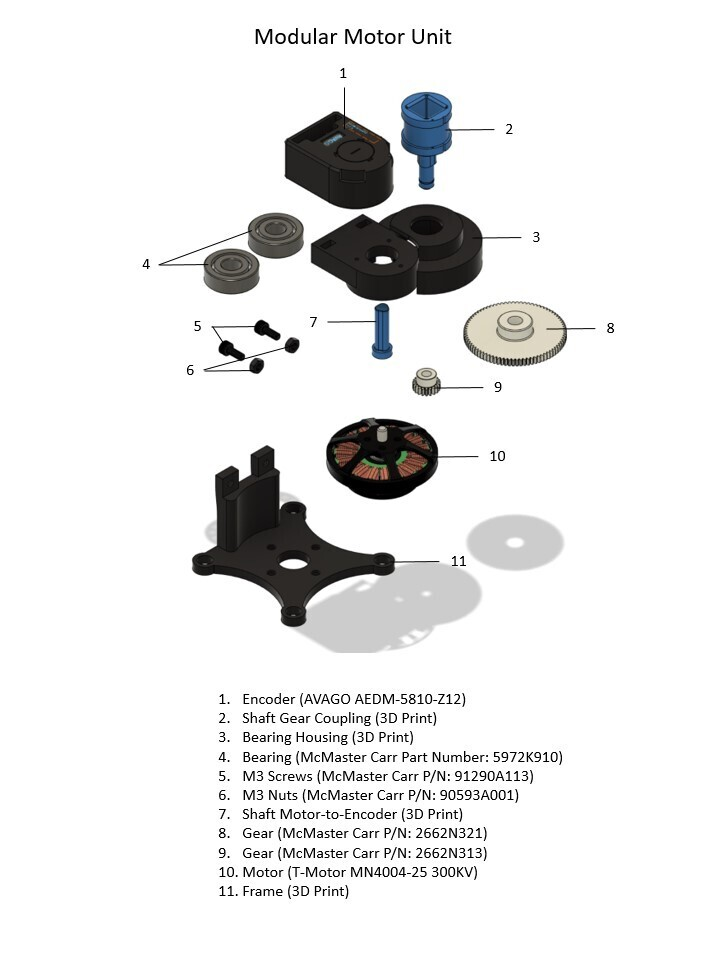
\includegraphics[width=\textwidth]{images/motor_unit.jpg}
    \caption{Complete schematic of the motor actuation unit, from \cite{motor_actuation_paper}}
    \label{fig:motor_unit}
\end{figure}

\paragraph{The workstation} used is a Dell OptiPlex 7090. It boasts an Intel Core i7-10700 CPU with 16GB of memory. It runs the RT-Preempt real time Linux kernel. The station communicates with the TI micro-controllers through a CAN-to-PCI Express interface card (IPEH-003027, PEAK system, Hessen, Germany). The station interfaces with the Aurora tracker through USB. Because the code for this thesis is written in Python, use of the real time kernel is not strictly required as Python does not support real time operations. For this project Python was deemed an appropriate language as it enables faster development times, and the shortcoming in terms of runtime is not seen to cause issues on the system. 

\subsubsection{Maximum Curvature Test}
Before the 16:1 gearbox was designed and installed, the actuation unit had a 4:1 gear ratio. An experiment was conducted to determine the arm length that enabled the largest range in the end effector position. Knowing the maximum and minimum distance that can be reached from an arm's base is required to set workspace bounds for the robot controller. The maximum distance is trivially given by the length of the arm. To find the minimum distance, a maximum curvature is applied by sending the highest current command a motor can support. The curvature that equates the bending forces to the maximum motor torque is taken as the maximum curvature. In this position, the distance between the end effector and arm base was measured. The results are displayed in Table \ref{tab:arm_length} and Figure \ref{fig:maximum_curve}. The arms were left at \SI{80}{cm} length as no notable gain in performance was observed at either test length. 

\begin{table}[h]
    \centering
    \caption{Arm distances during the maximum curvature test}
    \begin{tabular}{c|c|c}
        Extended Distance & Fully Contracted Distance & Contraction Distance \\
        \hline
        \SI{80}{cm} & \SI{59(1)}{cm} & \SI{21(1)}{cm} \\
        \SI{55}{cm} & \SI{33(1)}{cm} & \SI{22(1)}{cm} \\
    \end{tabular}
    \label{tab:arm_length}
\end{table}

This experiment showed the torque output of the motors resulted in a significantly smaller range of motion than what was initially expected. In response, a new gearbox was designed and manufactured to increase the maximum torque output of the robot. With the new gearbox, the robot is able to contract its arm completely with \SI{0}{cm} between the end effector and base. 

\begin{figure}[H]
     \centering
     \begin{subfigure}[b]{0.48\textwidth}
         \centering
         \includegraphics[width=\textwidth]{images/max_curve1.png}
         \caption{Without gearbox}
         \label{fig:maximum_curve1}
     \end{subfigure}
     \hfill
     \begin{subfigure}[b]{0.48\textwidth}
         \centering
         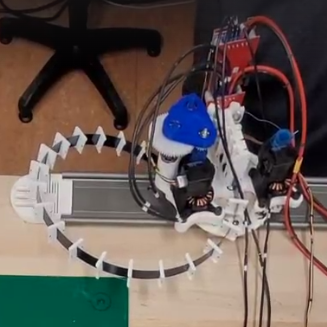
\includegraphics[width=\textwidth]{images/max_curve2.png}
         \caption{With gearbox}
         \label{fig:maximum_curve2}
     \end{subfigure}
        \caption{Maximum curvature tests}
        \label{fig:maximum_curve}
\end{figure}


\subsection{Baseline Controllers}
\label{sec:baseline_comparison}
Both the differential CC and PID baseline controllers were tested on three tasks: following a path, following a trajectory, and repeated the same motion. The results for each are presented in the following sections. The runtime of each controller is presented as well. 

\subsubsection{Path Tracking}
Both baseline controllers were asked to follow five test paths. Each path is discretized into ~50 way points. The controllers are required to measure an end effector position within \SI{2}{cm} of each way point before progressing to the next. The paths traced by each controller is shown in Figures \ref{fig:diff_cc_point_track} and \ref{fig:pid_point_track}. Table \ref{tab:baseline_test_point} highlights key metrics from each run including the total distance travelled by the robot and the time it took to complete each path. This test was repeated three times and the average results across all three trials are displayed. 

\begin{figure}[p]
    \centering
    \makebox[\textwidth][c]{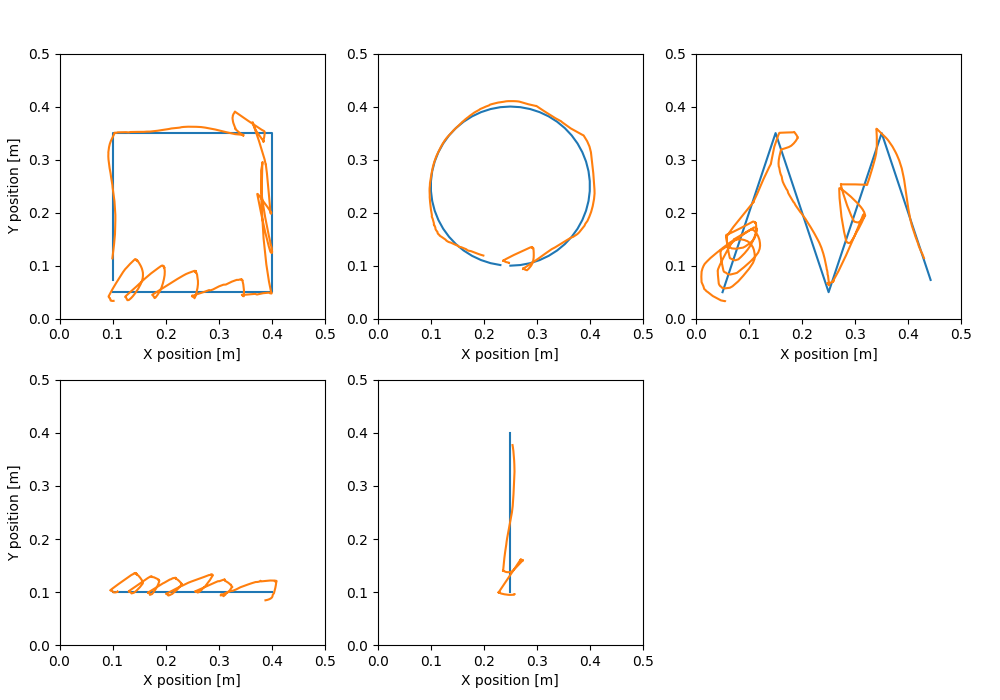
\includegraphics[width=0.95\textwidth]{images/diff_cc_point_tracking.png}}
    \caption{Differential CC controller point tracking path (orange) with reference path (blue) }
    \label{fig:diff_cc_point_track}
\end{figure}

\begin{figure}[p]
    \centering
    \makebox[\textwidth][c]{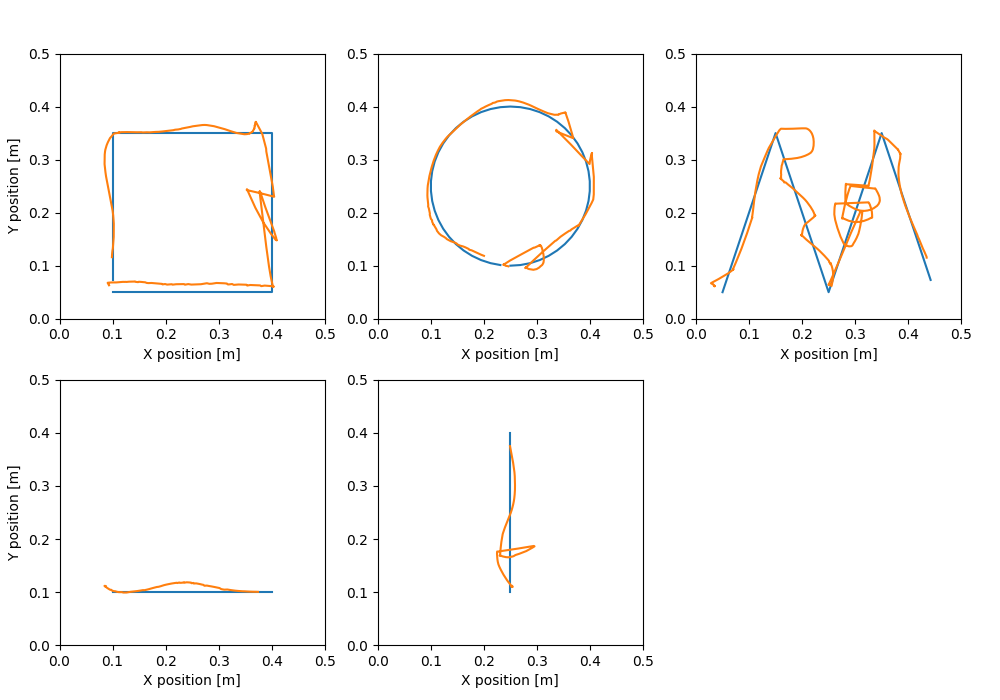
\includegraphics[width=0.95\textwidth]{images/pid_point_tracking.png}}
    \caption{PID controller point tracking path (orange) with reference path (blue)}
    \label{fig:pid_point_track}
\end{figure}

\begin{table}[h]
    \centering
    \caption{Baseline controller point tracking trial summary}
    \begin{tabular}{p{0.27\linewidth} | p{0.17\linewidth} | p{0.2\linewidth} | p{0.2\linewidth}}
        \textbf{Trial Shape} & \textbf{Run time [s]} & \textbf{Path Length [m]} & \textbf{Error}\\
        \hline
        \multicolumn{4}{c}{Reference Trajectory} \\
        \hline
        Square & N/A & 1.178 & N/A \\
        Circle & N/A & 0.923 & N/A \\
        Zig Zag & N/A & 1.241 & N/A \\
        Horizontal Line & N/A & 0.300 & N/A \\
        Vertical Line & N/A & 0.300 & N/A \\
        \hline
        \multicolumn{4}{c}{Differential CC Controller} \\
        \hline
        Square & 136.36 & 2.190 & 85.9\%\\
        Circle & 61.48 & 1.048 & 13.5\%\\
        Zig Zag & 152.21 & 2.551 & 105.6\%\\
        Horizontal Line & 105.48 & 0.817 & 172.3\%\\
        Vertical Line & 34.03 & 0.411& 37.0\%\\
        \hline
        \multicolumn{4}{c}{PID Controller} \\
        \hline
        Square & 74.92 & 1.454 & 23.4\%\\
        Circle & 87.58 & 1.197 & 29.7\%\\
        Zig Zag & 127.87 & 1.988& 60.2\%\\
        Horizontal Line & 19.01 & 0.302 & 0.6\%\\
        Vertical Line & 30.10 & 0.435 & 45\%\\
        \hline
    \end{tabular}   
    \label{tab:baseline_test_point}
\end{table}


\subsubsection{Trajectory Tracking}
Both baseline controllers were asked to execute five test trajectories in a set amount of time. Each trajectory is discretized into ~50 way points with \SI{0.2}{s} in between each. The robot is controlled to follow the way point as it progresses through each of the discretized points. The paths traced by each controller is shown in Figures \ref{fig:diff_cc_traj_track} and \ref{fig:pid_traj_track}. Table \ref{tab:baseline_test_traj} highlights key metrics from each run including the total distance travelled by the robot and the RMSE between the robot path and the test trajectory. 

\begin{figure}[p]
    \centering
    \makebox[\textwidth][c]{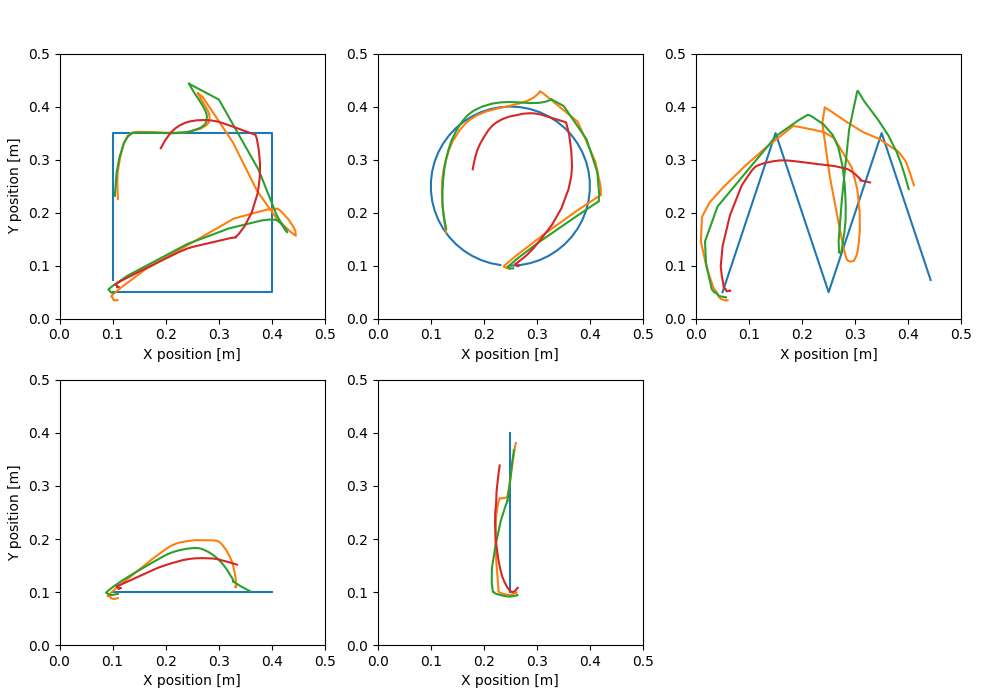
\includegraphics[width=0.95\textwidth]{images/diff_cc_traj_tracking.png}}
    \caption{Differential CC controller trajectory tracking paths (orange, green, red) with reference path (blue)}
    \label{fig:diff_cc_traj_track}
\end{figure}

\begin{figure}[p]
    \centering
    \makebox[\textwidth][c]{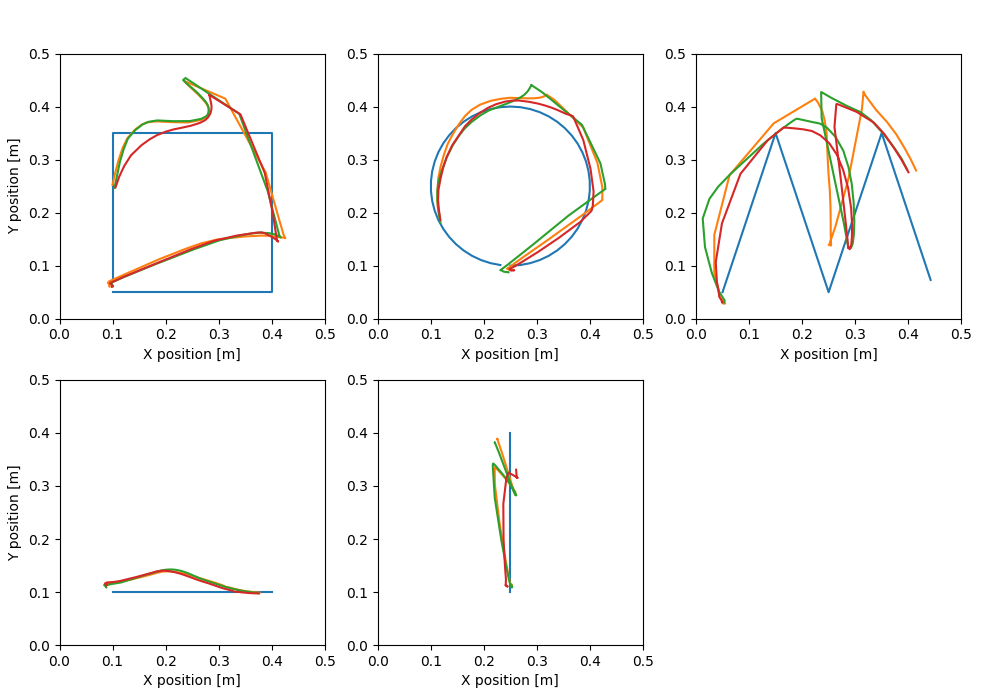
\includegraphics[width=0.95\textwidth]{images/pid_traj_tracking.png}}
    \caption{PID controller trajectory tracking paths (orange, green, red) with reference path (blue)}
    \label{fig:pid_traj_track}
\end{figure}

\begin{table}[h]
    \centering   
    \caption{Baseline controller trajectory tracking trial summary}
    \begin{tabular}{p{0.25\linewidth} | p{0.18\linewidth} | p{0.23\linewidth} | p{0.16\linewidth}}
        \textbf{Trial Shape} & \textbf{Run time [s]} & \textbf{Path Length [m]} & \textbf{RMSE [m]} \\
        \hline
        \multicolumn{4}{c}{Reference Trajectory} \\
        \hline
        Square & 10.80 & 1.178 & N/A\\
        Circle & 10.00 & 0.923 & N/A\\
        Zig Zag & 10.40 & 1.241 & N/A\\
        Horizontal Line & 10.20 & 0.300 & N/A\\
        Vertical Line & 10.20 & 0.300 & N/A\\
        \hline
        \multicolumn{4}{c}{Differential CC Controller} \\
        \hline
        Square & 12.25 & 0.959 & 0.144 \\
        Circle & 11.34 & 0.748 & 0.137 \\
        Zig Zag & 11.80 & 1.008 & 0.147 \\
        Horizontal Line & 11.57 & 0.324 & 0.072 \\
        Vertical Line & 11.57 & 0.305 & 0.055 \\
        \hline
        \multicolumn{4}{c}{PID Controller} \\
        \hline
        Square & 12.22 & 1.031 & 0.131 \\
        Circle & 11.31 & 0.833 & 0.124 \\
        Zig Zag & 11.77 & 11.213 & 0.150 \\
        Horizontal Line & 11.54 & 0.306 & 0.043 \\
        Vertical Line & 11.54 & 0.360 & 0.054 \\
        \hline
    \end{tabular}
    \label{tab:baseline_test_traj}
\end{table}


\subsubsection{Task Repetition}
Controllers were tested on their ability to repeat the same task consistently. The trial was run from home position to the point (\SI{0.15}{m}, \SI{0.2}{m}). It was repeated 10 times for each controller. The paths taken by each controller are shown in Figure \ref{fig:repetition_trial}. The maximal Fréchet distance \cite{frechet_distance} is calculated between each of the 10 trials for both controllers as a metric of controller consistency. The differential CC controller has a maximal Fréchet distance of \SI{0.102}{m} while the PID controller has a maximal Fréchet distance of \SI{0.027}{m}, indicating a much tighter distribution. This result is confirmed visually in Figure \ref{fig:repetition_trial}. 

\begin{figure}[h]
     \centering
     \begin{subfigure}[b]{0.48\textwidth}
         \centering
         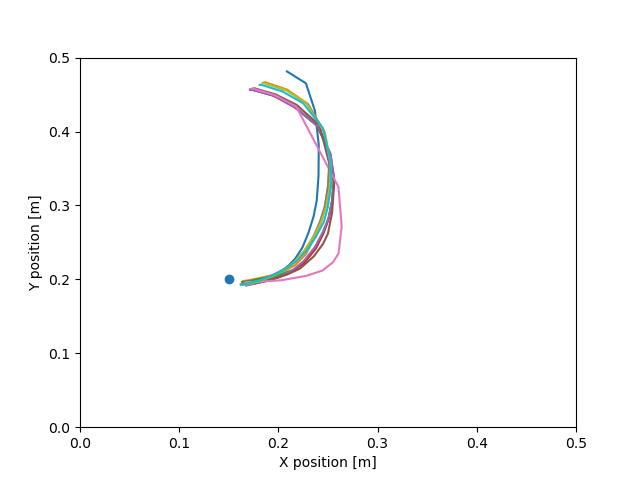
\includegraphics[width=\textwidth]{images/diff_cc_repetition.png}
         \caption{Differential CC controller task repetition}
         \label{fig:diff_cc_repetition}
     \end{subfigure}
     \hfill
     \begin{subfigure}[b]{0.48\textwidth}
         \centering
         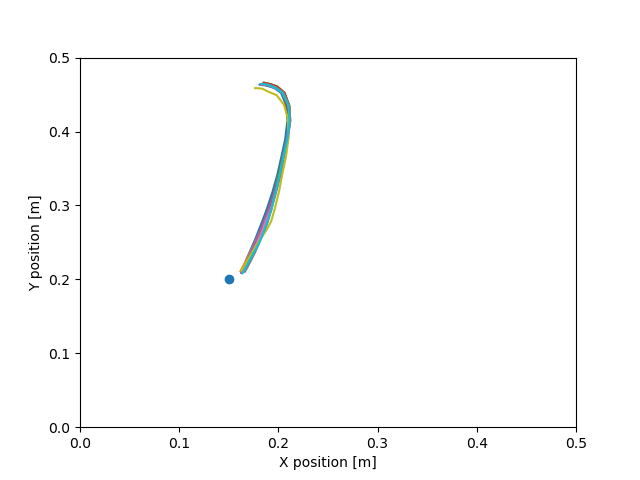
\includegraphics[width=\textwidth]{images/pid_repetition.png}
         \caption{PID controller task repetition}
         \label{fig:pid_repetition}
     \end{subfigure}
        \caption{Baseline controller repeated motion trial paths. The target point is shown in blue.}
        \label{fig:repetition_trial}
\end{figure}


\subsubsection{Timing Analysis}
The runtime of four different necessary controller functions was studied for both baseline controllers and the best performing learned controller. This includes the controller constructor method, the command retrieval, the end point update, and the goal point update. Table \ref{tab:runtimes} displays the results. A "per iteration" result is returned as well, which is a sum of the three functions that are required to run at each control loop. 

\begin{table}[h]
    \centering   
    \caption{Controller run times}
    \begin{tabular}{p{0.4\linewidth} | p{0.2\linewidth} }
        \textbf{Function} & \textbf{Run time [$\mu$s]} \\
        \hline
        \multicolumn{2}{c}{Differential CC Controller} \\
        \hline
        Current command retrieval & 0.1 \\
        End point update & 364.2 \\
        Goal point update & 0.2 \\
        \textbf{Total per iteration} & \textbf{364.5} \\
        Controller object construction & 11.4 \\
        \hline
        \multicolumn{2}{c}{PID Controller} \\
        \hline
        Current command retrieval & 0.1 \\
        End point update & 24.5 \\
        Goal point update & 0.8 \\
        \textbf{Total per iteration} & \textbf{25.4} \\
        Controller object construction & 211.0 \\
        \hline
        \multicolumn{2}{c}{Learning-Based Controller} \\
        \hline
        Current command retrieval & 0.2 \\
        End point update & 356.3 \\
        Goal point update & 0.2 \\
        \textbf{Total per iteration} & \textbf{356.7} \\
        Controller object construction & 1,184.3 \\
        \hline
    \end{tabular}
    \label{tab:runtimes}
\end{table}


\subsection{Data Set}
Over a span of three days, data was collected using the methods outlined in Section \ref{sec:data_methods}. A total runtime of \SI{5.78}{h} was collected. The robot traveled \SI{472}{m} and broke down four times. 

\subsubsection{Distributions}
Presented in this section is both the task space and joint space distributions of the dataset. In task space, the position, velocity, and acceleration of the end effector are displayed in the histogram in Figure \ref{fig:dataset_dist_task}. In joint space, the motor current is displayed along with the motor current's first and second derivatives in Figure \ref{fig:dataset_dist_joint}. 

\begin{figure}[h]
    \centering
    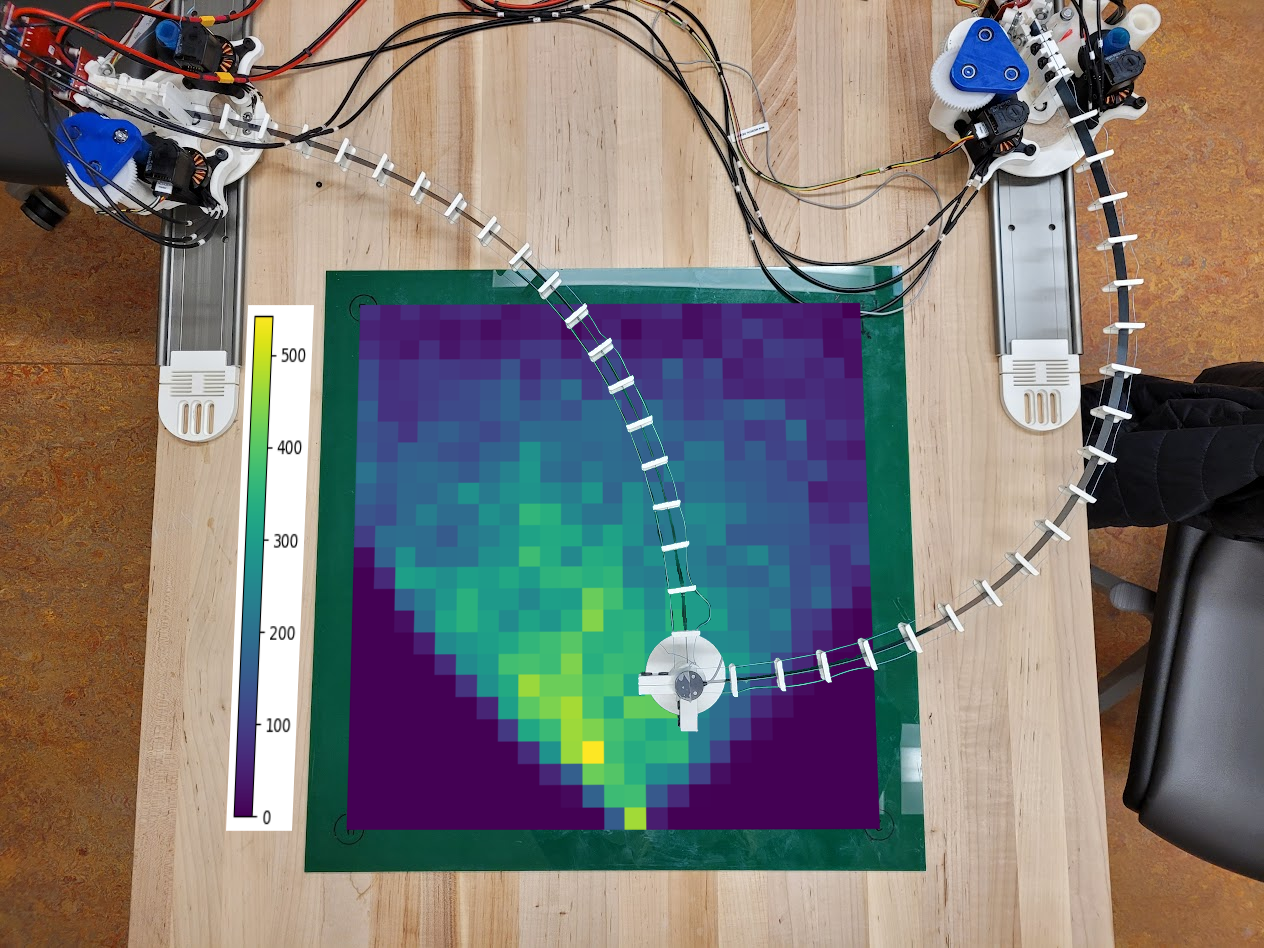
\includegraphics[width=\textwidth]{images/dataset_overlay.png}
    \caption{Data set position distribution overlaid on robot workspace}
    \label{fig:dataset_overlay}
\end{figure}

Figure \ref{fig:dataset_overlay} shows the task space position distribution overlaid on the robot's workspace. The densest distribution point at the middle-bottom of the workspace corresponds with the robot's home position. This is where the robot starts each time it is powered on and where it returns to in recovery mode. 

\begin{figure}[h]
     \centering
     \begin{subfigure}[b]{0.48\textwidth}
         \centering
         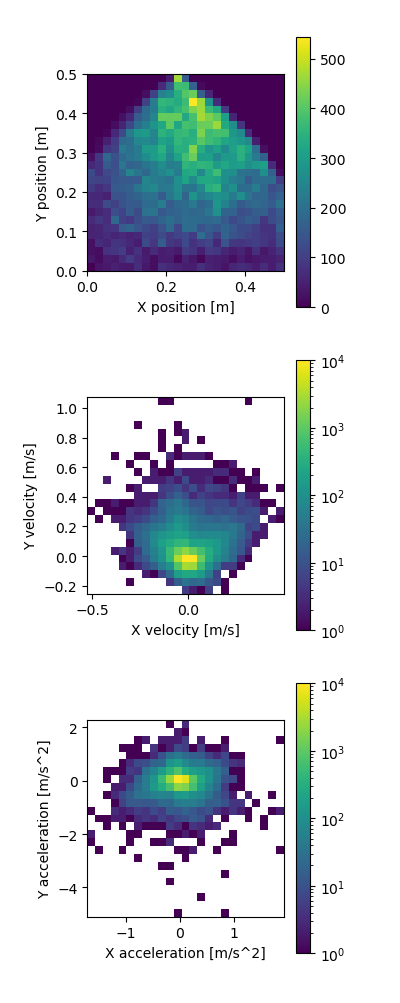
\includegraphics[width=\textwidth]{images/dataset_distribution.png}
         \caption{Task space distribution}
         \label{fig:dataset_dist_task}
     \end{subfigure}
     \hfill
     \begin{subfigure}[b]{0.48\textwidth}
         \centering
         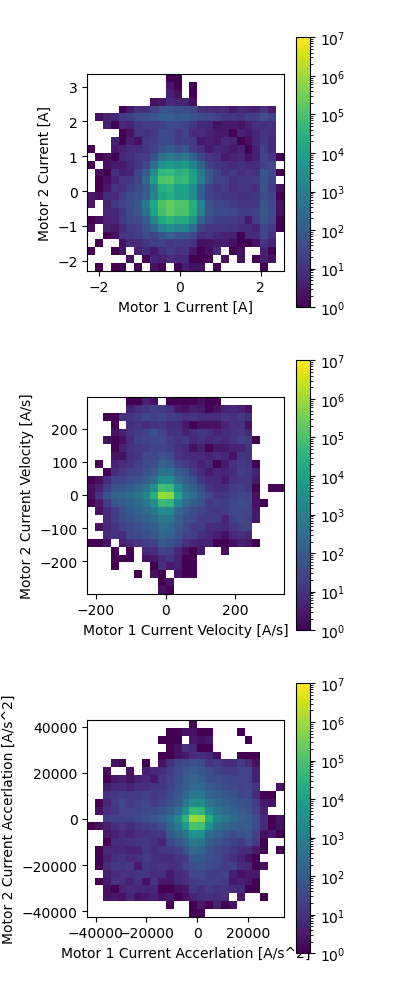
\includegraphics[width=\textwidth]{images/dataset_distribution_joint.png}
         \caption{Joint space distribution}
         \label{fig:dataset_dist_joint}
     \end{subfigure}
        \caption{Data set distribution histograms}
        \label{fig:dataset_dist}
\end{figure}

Table \ref{tab:dataset_runtype} breaks down the sample termination cases for the dataset, along with relevant metrics for each. Note that all cases that ended in an error termination were manually removed due to data corruption. 

\begin{table}[h]
    \centering
    \caption{Data set run type summary}
    \makebox[\textwidth][c]{\begin{tabular}{p{0.15\linewidth} | p{0.12\linewidth} | p{0.12\linewidth} | p{0.12\linewidth} | p{0.14\linewidth} | p{0.12\linewidth} | p{0.1\linewidth}}
        \textbf{Data Run Type} & \textbf{Average Distance [m]} & \textbf{Average Velocity [m/s]}  & \textbf{Average Duration [s]}  & \textbf{Total Distance [m]} & \textbf{Total Duration [s]} & \textbf{Total Runs}\\
        \hline
        Success & 0.1038 & 0.0294 & 4.49 & 367.78 & 15,915 & 3543\\
        \hline
        Stalled & 0.1142 & 0.0184 & 6.55 & 73.29 & 4,203 & 642\\
        \hline
        Aurora Lost & 0.1281 & 0.0338 & 3.65 & 1.79 & 51 & 14\\
        \hline
        Recovery & 0.3962 & 0.0591 & 6.69 & 22.77 & 401 & 60\\
        \hline
        Mode Switched & 0.1157 & 0.0322 & 4.66 & 5.44 & 219 & 47\\
        \hline
        User Terminated & 0.0811 & 0.0217 & 3.42 & 0.16 & 7 & 2\\ 
    \end{tabular}}
    \label{tab:dataset_runtype}
\end{table}
\subsection{Deep-Learning Controller}


\subsubsection{Model Architectures}
A number of model architectures were trained in a coarse to fine grid sweep to determine an optimal learning model baseline for future experiments. A summary of the trial results is displayed in Table \ref{tab:arch_search}. Only the best architecture from each trial is shown. For a full breakdown of each trial, see Appendix \ref{app:learning}. In many trials a clear winner is not found, and changing the parameter has little to no effect on the model performance. In these cases, the baseline model selection criteria favours smaller parameters to enable faster run times. 

\begin{table}[h]
    \centering
    \caption{Model architecture search trial summary}
    \makebox[\textwidth][c]{\begin{tabular}{p{0.32\linewidth} | p{0.15\linewidth} | p{0.15\linewidth} | p{0.12\linewidth} | p{0.16\linewidth}  }
        \textbf{Trial Type} & \textbf{Backbone Linear Layer Size(s)} & \textbf{Head Linear Layer Size(s)} & \textbf{LSTM Layer Size} & \textbf{Best RMSE Validation Loss [A]} \\
        \hline
        LSTM layer size search & 10, 10 & 50 & 15 & 0.0220 \\
        Head layer size search & 10, 10 & 0 & 20 & 0.0226 \\
        Head layer depth search & 10, 10 & 25, 25 & 20 & 0.0224 \\
        Backbone layer size search & 30 & 25, 25 & 20 & 0.0205 \\
        Backbone layer depth search & 20, 20 & 25, 25 & 15 & 0.0221 \\
    \end{tabular}}
    \label{tab:arch_search}
\end{table}

The baseline configuration chosen for future trials contains a backbone with two fully connected layers of 10 nodes each, an LSTM state estimator with 30 nodes, and a single fully connected head layer with 100 nodes. Other baseline parameters include: 512 batch size, 1000 epochs, 0.001 learning rate, a \SI{0.2}{s} feedback horizon, and a \SI{0.2}{s} prediction horizon. 

\subsubsection{Feedback Horizon}
Figure \ref{fig:feedback_horizon} shows the model search for an optimal feedback horizon length. The model used for this trial is the baseline model described in Section \ref{sec:learning_baseline_description}. The feedback horizon was varied from \SI{0}{s} (no feedback data is provided) to \SI{15}{s}. The best validation loss achieved from a model trained using each given feedback horizon is presented. 

\begin{figure}[h]
    \centering
    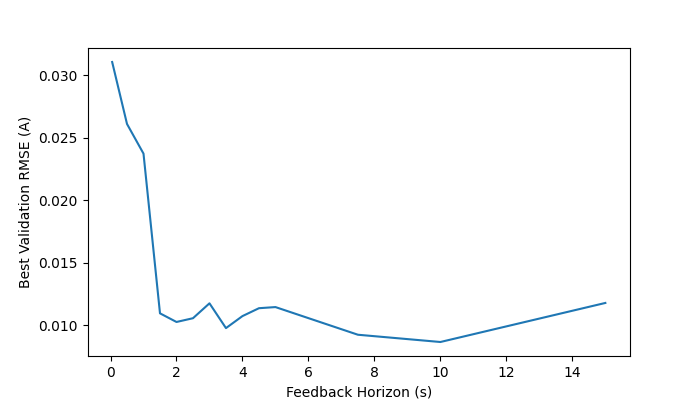
\includegraphics[width=0.75\textwidth]{images/feedback_horizon.png}
    \caption{Best validation losses in feedback horizon trial}
    \label{fig:feedback_horizon}
\end{figure}


\subsubsection{Configuration Parameters}
Figure \ref{fig:configuration_size} shows the model search for an optimal configuration parameter size. The model used for this trial is the baseline model described in Section \ref{sec:learning_baseline_description}. The configuration parameter size was varied from 0 (no configuration parameter is provided) to 20. The configuration parameter size refers to a set of tunable values passed as an input to the model where each set of values is unique to the robot configuration that the data was collected on. Each time the robot broke, a new configuration is labelled.

\begin{figure}[h]
    \centering
    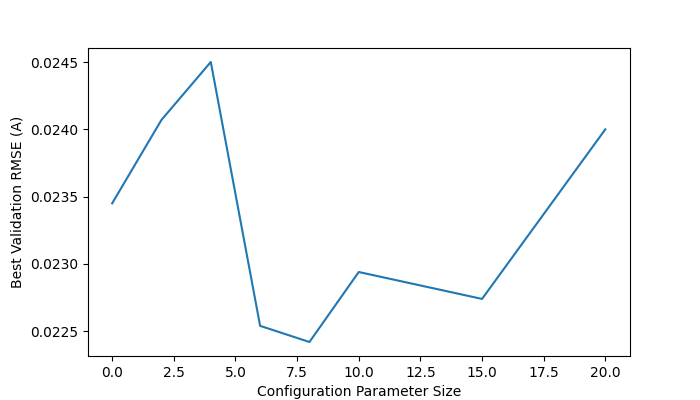
\includegraphics[width=0.75\textwidth]{images/configuration_size.png}
    \caption{Best validation losses in configuration parameter trial}
    \label{fig:configuration_size}
\end{figure}


\subsubsection{Data Weighting}
The data weighing trial compared model performance when trained using weighted prediction labels. Three weight distributions were tested alongside an unweighted baseline. Each weight function was trained with six different model architectures. The results of this trial are shown in Figure \ref{fig:prediction_weighting}. The weight for each trials are sampled from a continuous function defined on the prediction interval. Each set of weights is normalized so that the sum of all weights equals one. The functions used are defined in Table \ref{tab:weights}.

\begin{table}[h]
    \centering
    \caption{Data weight definitions for data weighing trial}
    \makebox[\textwidth][c]{\begin{tabular}{c | c | c}
        \textbf{Weight Class} & \textbf{Function (Pre-Normalization)} & \textbf{Interval}\\
        \hline
        Unweighted & $f(t) = 1$ & N/A\\
        Linear & $f(t) = \frac{t}{3}$ & $[1, 3)$ \\
        Exponential & $f(t) = e^t$ & $[0, 2)$\\
        Quadratic & $f(t) = t^2 - 1.5t + 1.5$ & $[0, 2)$
    \end{tabular}}
    \label{tab:weights}
\end{table}
    
\begin{figure}[h]
    \centering
    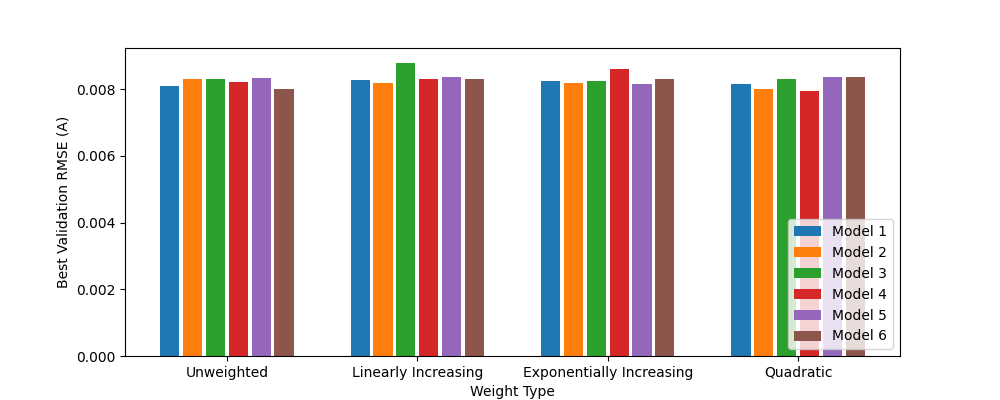
\includegraphics[width=0.95\textwidth]{images/prediction_weighting.png}
    \caption{Best validation losses in prediction weighting trial}
    \label{fig:prediction_weighting}
\end{figure}

\pagebreak
\section{Discussion}
\label{sec:discussion}

\subsection{Prototype Hardware}
% Add drawings / design philosophy 
The robot is designed with the Open Continuum Robotics project in mind. It uses easily accessible, off-the-shelf components, and 3D printed parts so that other groups can reconstruct the same robot. A full breakdown of the robot's physical design can be found in Appendix \ref{app:robot_drawings}. 

\subsubsection{Physical Description of Prototype}
\label{sec:physical_description}
% Arms
\paragraph{The arms} are each \SI{80}{cm} long and consist of a \SI{0.0200}{"} thick, \SI{0.75}{"} wide beam made from 1095 spring steel, with 19 evenly spaced 3D printed tendon spacers. The spacers hold one tendon on each side of the beam \SI{11}{mm} away from the steel beam. The 1095 spring steel beam is used as the central beam as it provides rigidity in the direction of motion off the robot's planar surface, while remaining flexible along the plane. The high elasticity of the material allows the system to undergo large curvatures without permanently deforming the beam. The tendons used are \SI{30}{lbs} braided fishing line (Super8Slick V2, Power Pro, CA, USA). Each tendon has four \SI{0.75}{"} nuts on it that act to maintain tension during operational periods where it is being extended. 

\begin{figure}[h]
    \centering
    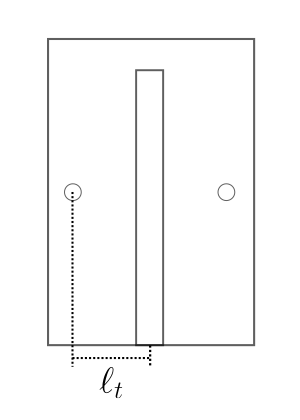
\includegraphics[width=0.3\textwidth]{images/beam_cross_section.png}
    \caption{Cross section of the beam spacers. $\ell_t = \SI{11}{mm}$}
    \label{fig:beam_cross_section}
\end{figure}

\begin{figure}[h]
    \centering
    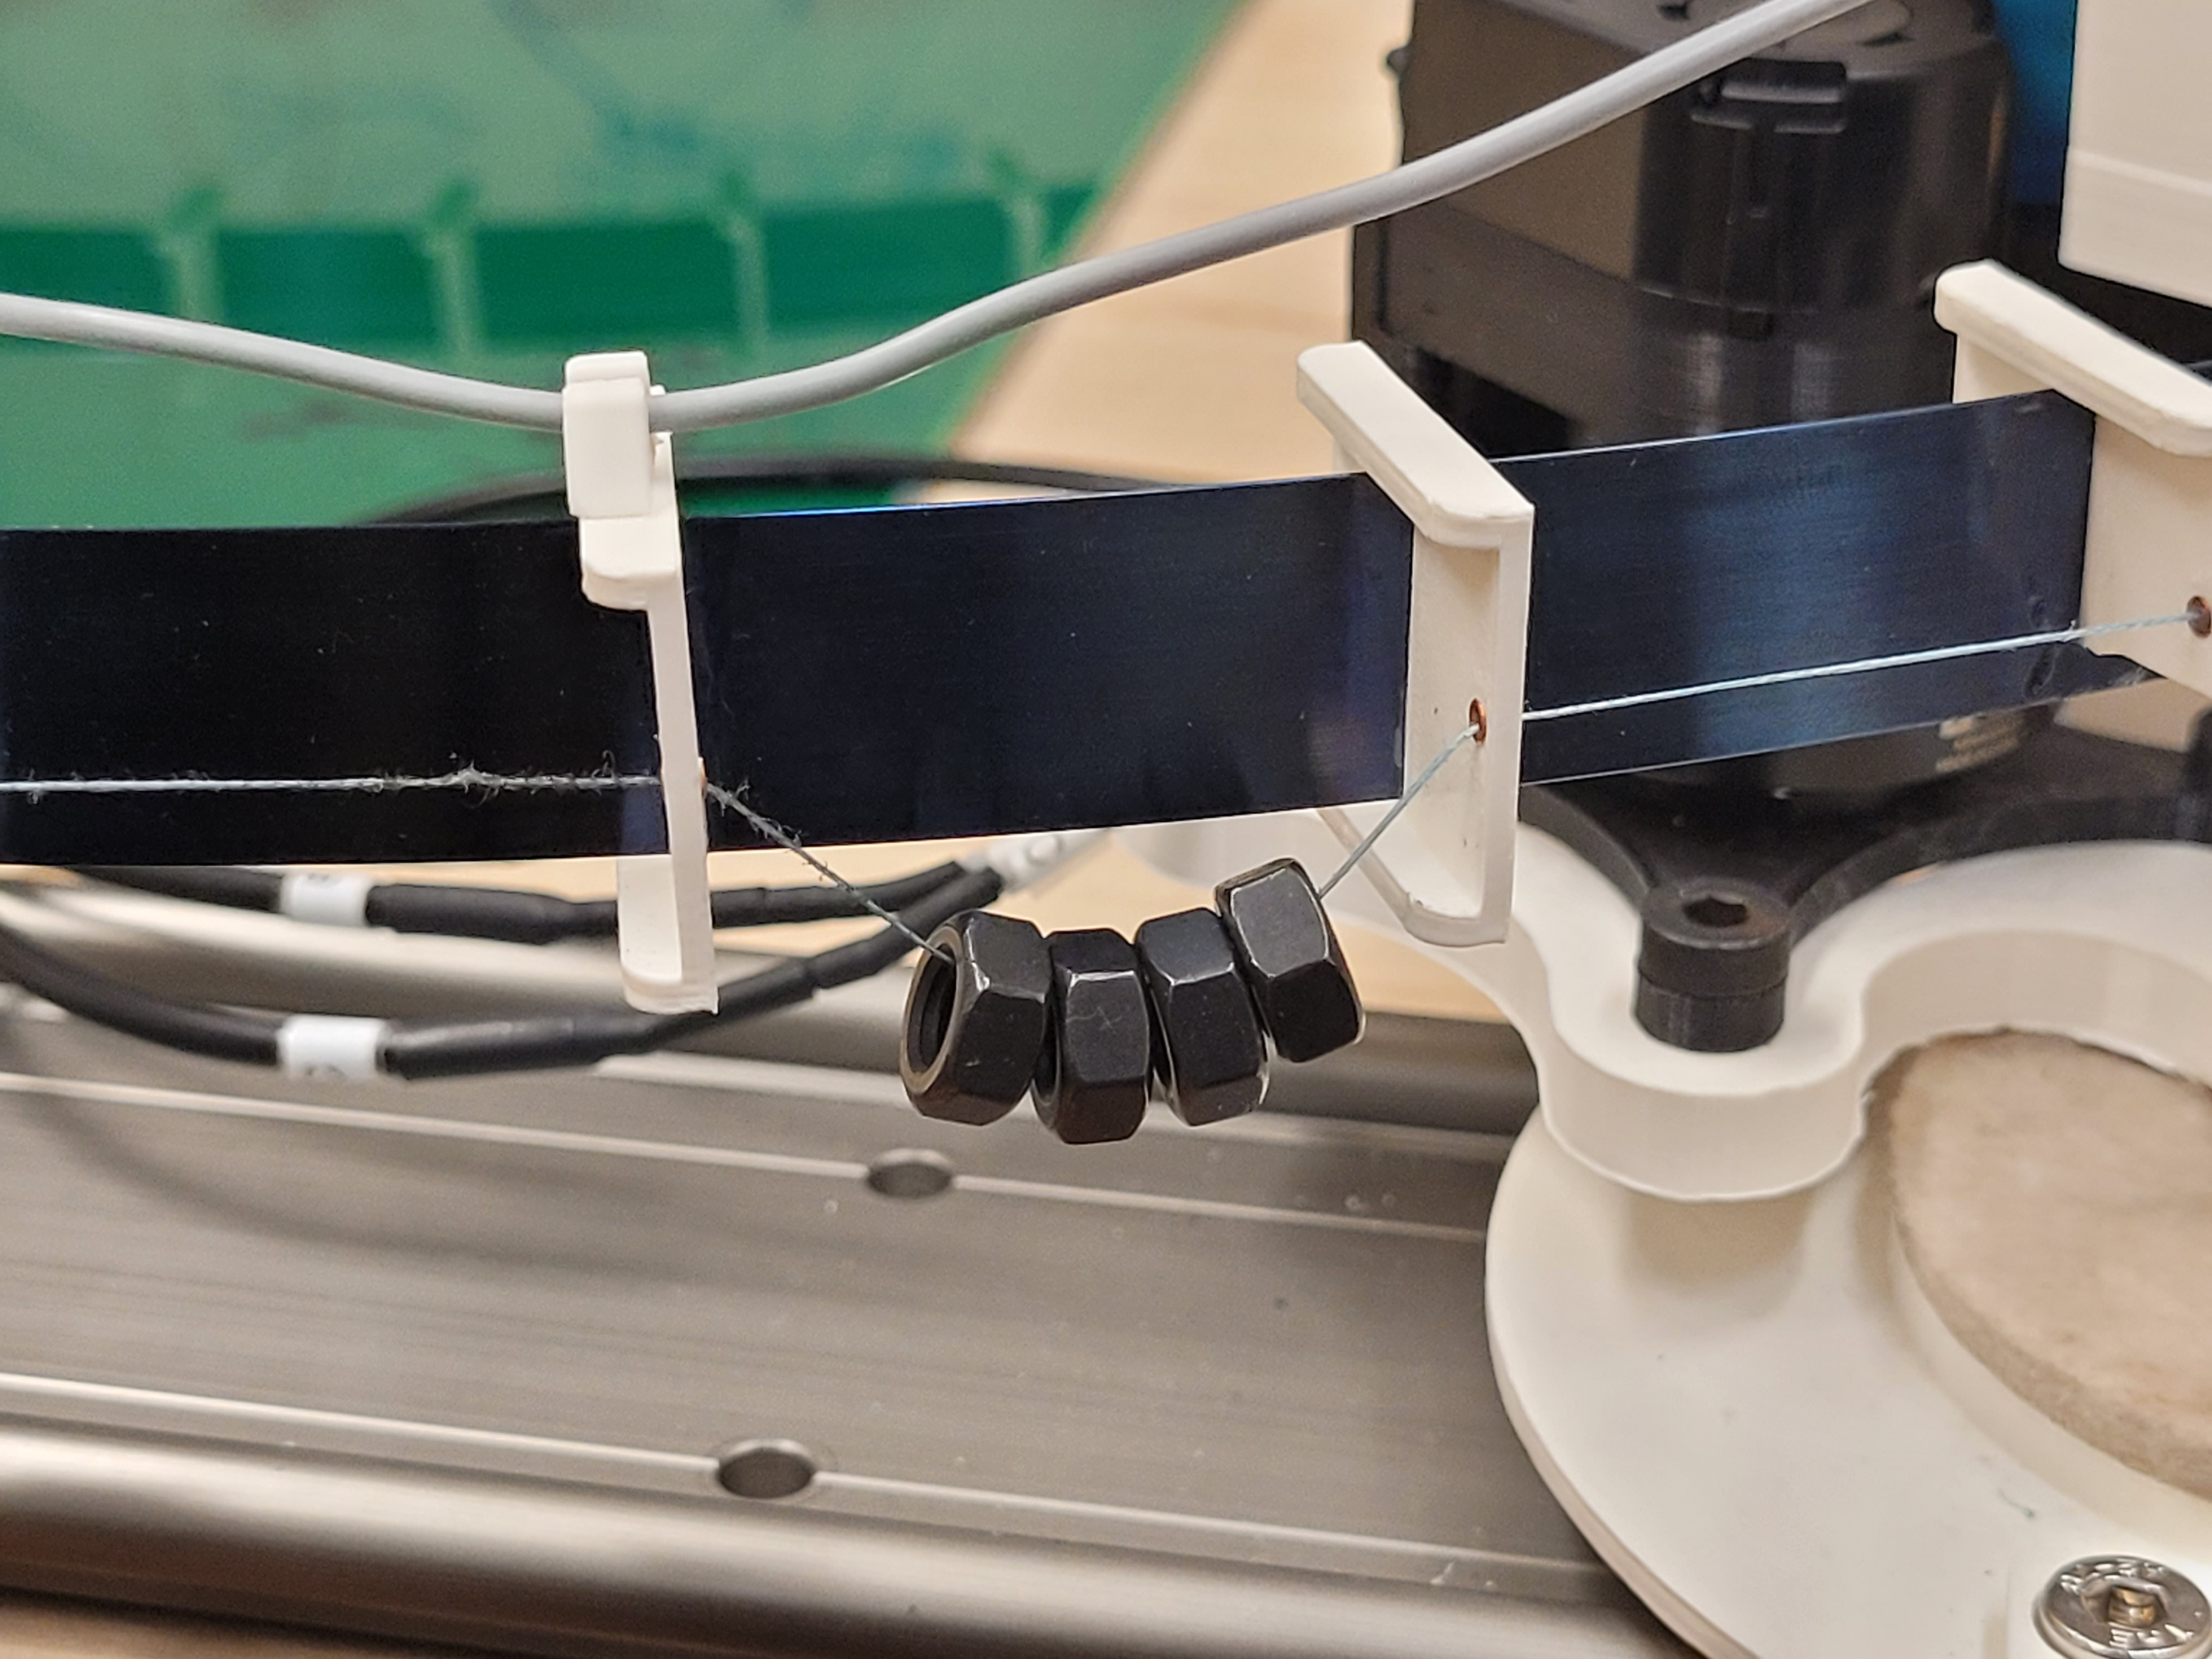
\includegraphics[width=0.5\textwidth]{images/tendon_slack.jpg}
    \caption{Four \SI{0.75}{"} nuts placed on a tendon to maintain tendon tension throughout operation}
    \label{fig:tendon_slack}
\end{figure}

% \begin{figure}[h]
%      \centering
%      \begin{subfigure}[b]{0.48\textwidth}
%          \centering
%          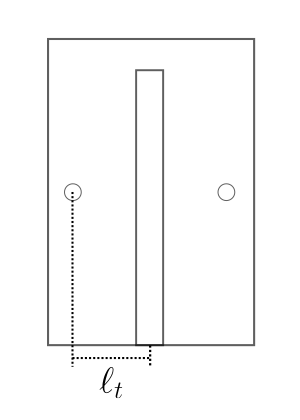
\includegraphics[width=0.625\textwidth]{images/beam_cross_section.png}
%          \caption{Cross section of the beam spacers. $\ell_t = \SI{11}{mm}$}
%          \label{fig:beam_cross_section}
%      \end{subfigure}
%      \hfill
%      \begin{subfigure}[b]{0.48\textwidth}
%          \centering
%          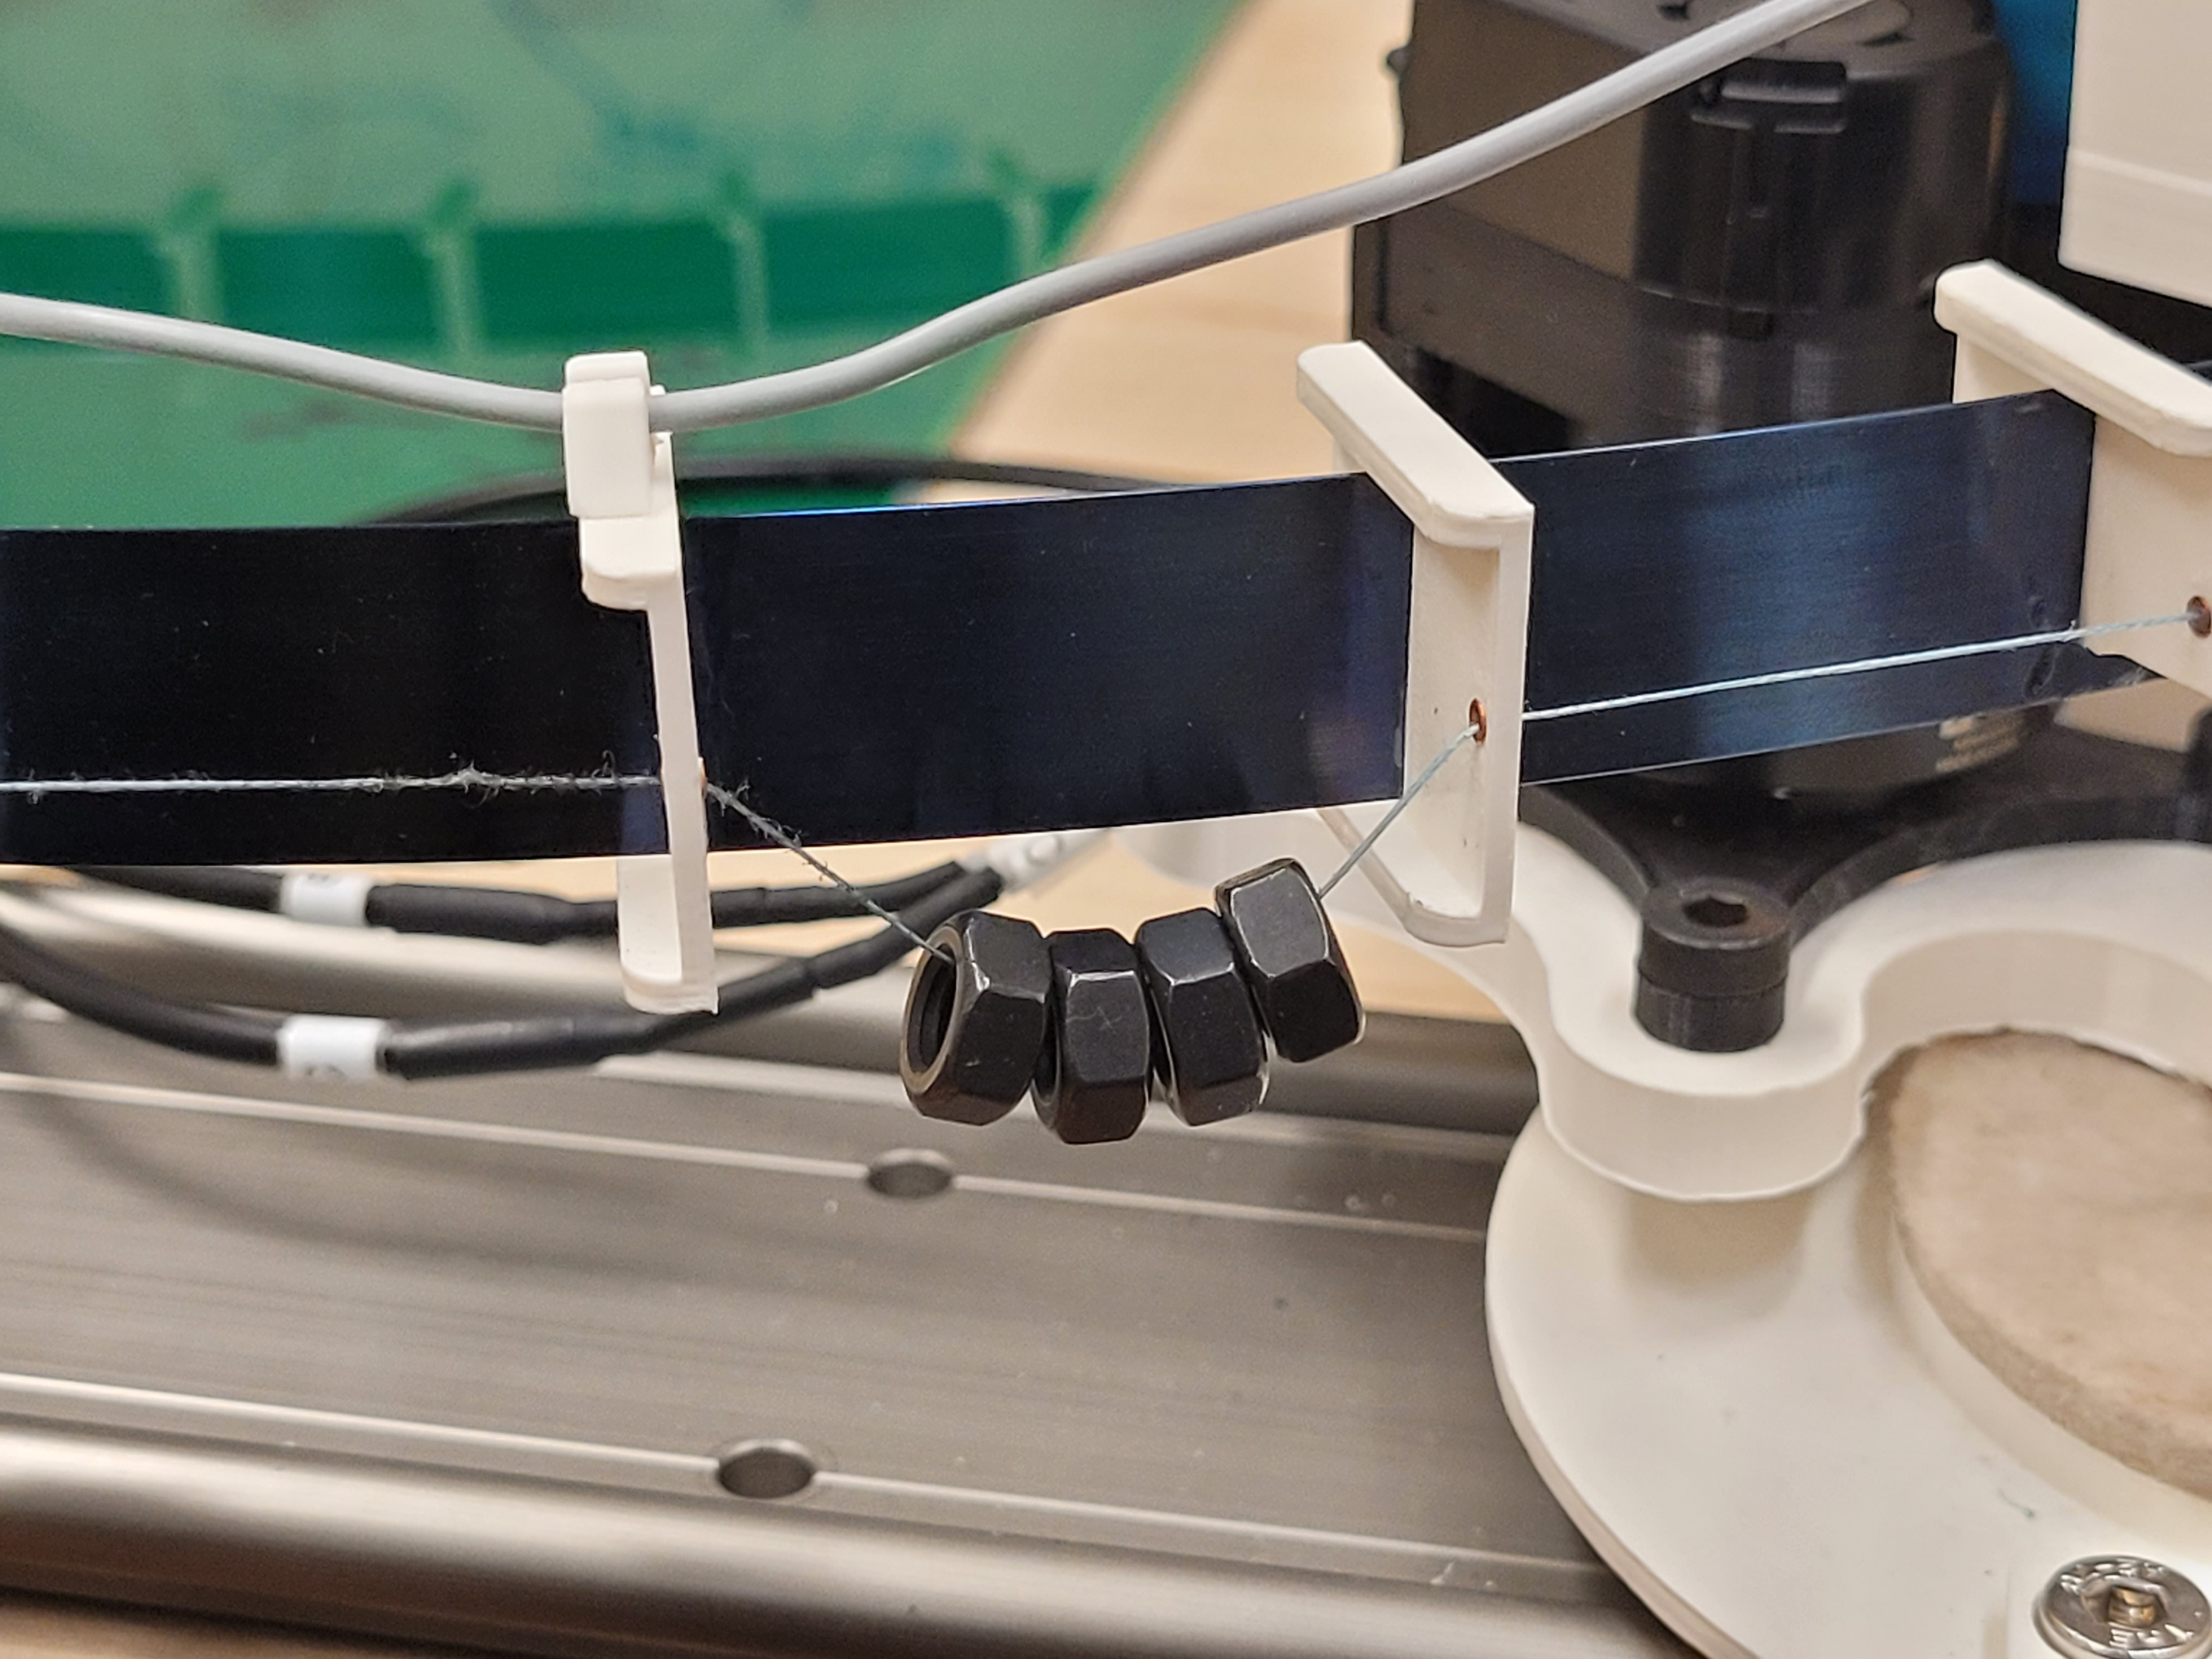
\includegraphics[width=\textwidth]{images/tendon_slack.jpg}
%          \caption{Four \SI{0.75}{"} nuts placed on a tendon to maintain tendon tension throughout operation}
%          \label{fig:tendon_slack}
%      \end{subfigure}
% \end{figure}

% Joints and End Effector  
\paragraph{The end effector} features a wide base to prevent the end effector from twisting off the plane. Revolute joints link the ends of each arm to the motor bases and the end effector, allowing both ends to rotate freely about the z-axis. The two arms share the same end effector. The bases for each arm are positioned \SI{60}{cm} apart.Each arm having its own independent degree of freedom grants the end effector in this configuration two degrees of freedom laying on the table plane. At this distance, the reachable workspace of the end effector covers a majority of the AURORA tracker workspace. During operation, a smaller end effector base does not provide enough area to balance the moments being applied by the two arms actuating the piece from different heights. Figure \ref{fig:ee_comparison} demonstrates this effect in action. Felt pads are attached to the bottom of the end effector to reduce friction between the end effector and table surface. 

\begin{figure}[h]
     \centering
     \begin{subfigure}[b]{0.48\textwidth}
         \centering
         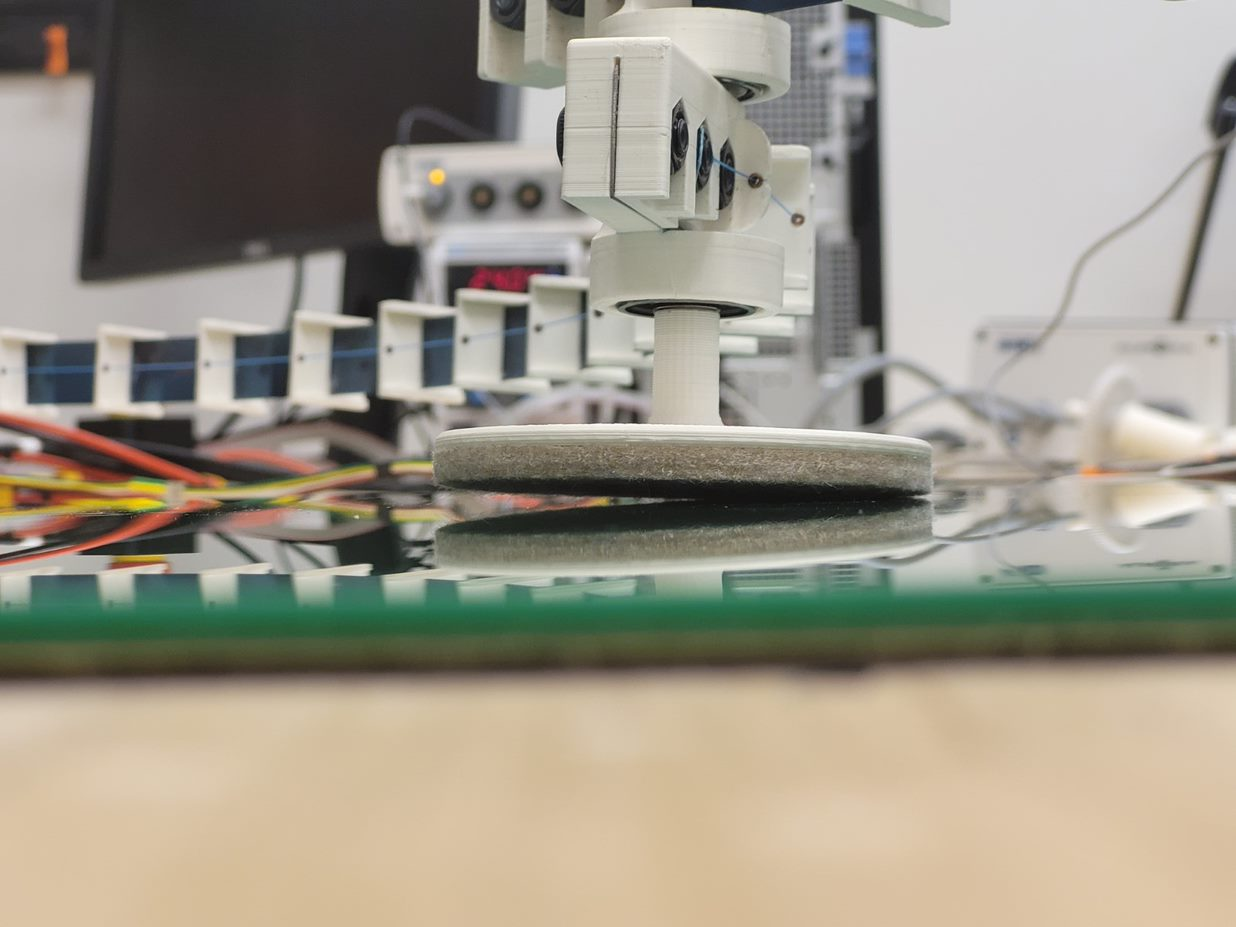
\includegraphics[width=\textwidth]{images/small_ee.jpeg}
         \caption{Smaller base causing the end effector to twist off the planar surface}
         \label{fig:small_ee}
     \end{subfigure}
     \hfill
     \begin{subfigure}[b]{0.48\textwidth}
         \centering
         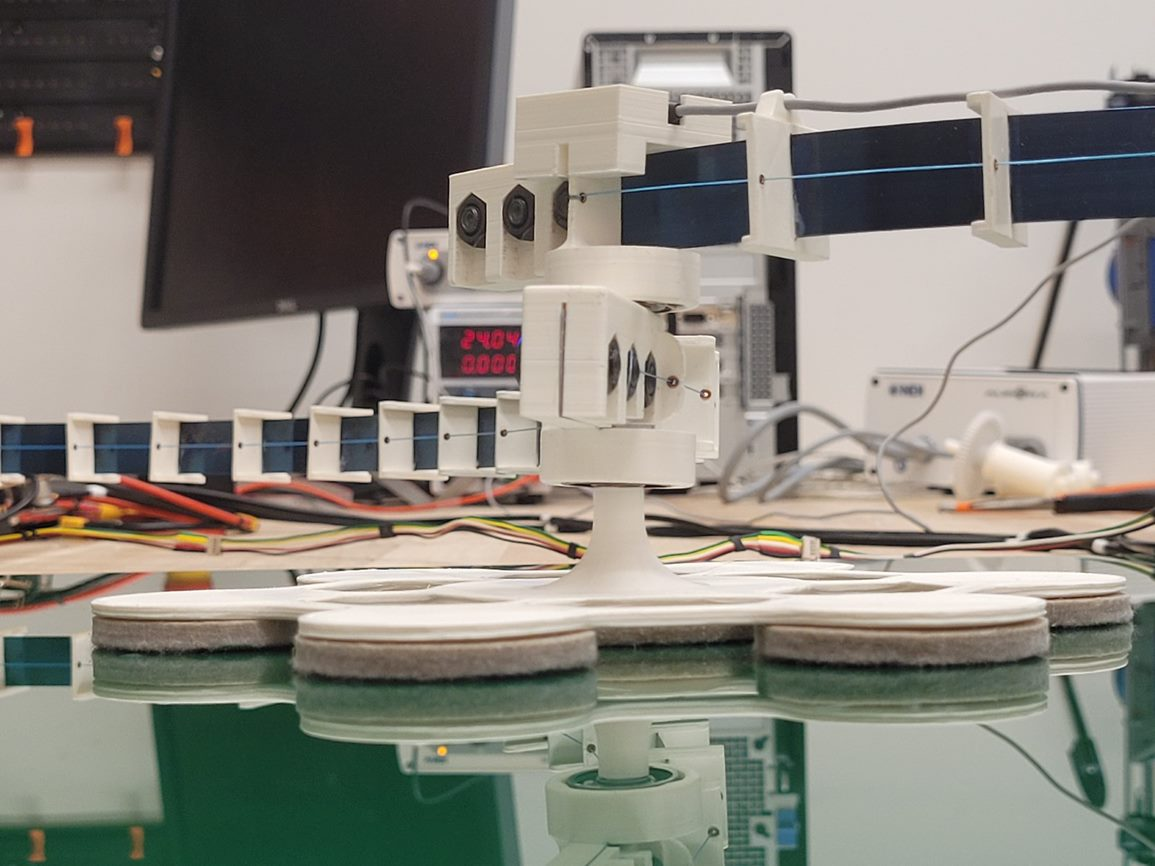
\includegraphics[width=\textwidth]{images/large_ee.jpeg}
         \caption{Larger base ensuring end effector remains on the plane}
         \label{fig:large_ee}
     \end{subfigure}
        \caption{Comparison of end effector sizes}
        \label{fig:ee_comparison}
\end{figure}

\paragraph{Gearboxes} are actuated directly by motors for each arm. The gear boxes are 3D printed but use purchase gears with a gear ratio of 16:1, enabling significantly higher applied torques than the motors are natively capable of. A 4:1 gear ratio is achieved by the motor unit. This results in a total gear ratio of 64:1 for the actuation unit. Each box contains two \SI{10}{mm} gears (2662N313, McMaster-Carr Supply Company, IL, USA) and three \SI{40}{mm} gears (2662N321, McMaster-Carr Supply Company, IL, USA) to achieve this rotation. The gearbox actuates a 3D printed spindle with a radius of \SI{11}{mm}. Two tendons are spooled around the spindle in opposite directions, so when it rotates, one tendon is extended while the other is contracted. Both tendons are firmly attached at the end effector side of each arm. This equal and opposite actuation of the tendons is what causes the arm to bend. 

% Workspace 
\paragraph{The workspace} additionally has an acrylic sheet used to reduce friction. Beneath the table surface, an AURORA electromagnetic tracking system (20-20 planar, Northern Digital Inc., ON, Canada) is positioned. The tracker is positioned to ensure maximal coverage of the robot's task space. The tracker is limited to an effective tracking area of \SI{50}{cm} x \SI{50}{cm} on the workspace plane. This unit tracks a wire coil which is fastened on the robot's end effector, directly above the revolute joint. This is where the end effector position is defined to be as a point in space. 

\subsubsection{Electronic Components}
Each arm is driven by a single Antigravity drone motor (MN4004 KV300, T-MOTOR, JX, P.R. China) which are both controlled by an off-the-shelf microprocessor (LAUNCHXL-F28069M, Texas Instruments, Dallas, USA) fitted with two booster cards (BOOSTXL-DRV8305EVM, Texas Instruments, Dallas, USA). The motors are part of an actuation unit shown in Figure \ref{fig:motor_unit} and contain a 4:1 gear ratio and an Avago optical encoder (AEDM 5810, Broadcom Inc., CA, USA) that is used to provide system feedback at a rate of \SI{1000}{hz} to the workstation. The actuation setup comes from the Open Continuum Robot project \cite{open_cr, Grimminger_2020}. A single micro-controller communicates with a workstation through the CAN bus protocol. The robot is powered using a \SI{240}{W} power supply operating at \SI{24}{V}. An emergency stop is installed within reach of the operator for safety. 

\begin{figure}[p]
    \centering
    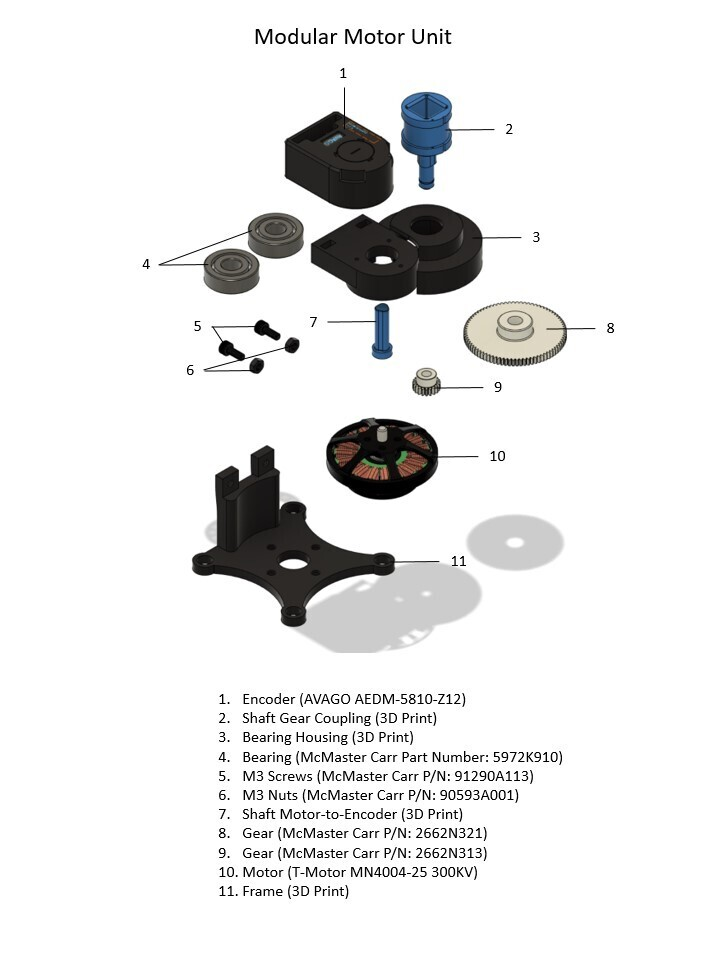
\includegraphics[width=\textwidth]{images/motor_unit.jpg}
    \caption{Complete schematic of the motor actuation unit, from \cite{motor_actuation_paper}}
    \label{fig:motor_unit}
\end{figure}

\paragraph{The workstation} used is a Dell OptiPlex 7090. It boasts an Intel Core i7-10700 CPU with 16GB of memory. It runs the RT-Preempt real time Linux kernel. The station communicates with the TI micro-controllers through a CAN-to-PCI Express interface card (IPEH-003027, PEAK system, Hessen, Germany). The station interfaces with the Aurora tracker through USB. Because the code for this thesis is written in Python, use of the real time kernel is not strictly required as Python does not support real time operations. For this project Python was deemed an appropriate language as it enables faster development times, and the shortcoming in terms of runtime is not seen to cause issues on the system. 

\subsubsection{Maximum Curvature Test}
Before the 16:1 gearbox was designed and installed, the actuation unit had a 4:1 gear ratio. An experiment was conducted to determine the arm length that enabled the largest range in the end effector position. Knowing the maximum and minimum distance that can be reached from an arm's base is required to set workspace bounds for the robot controller. The maximum distance is trivially given by the length of the arm. To find the minimum distance, a maximum curvature is applied by sending the highest current command a motor can support. The curvature that equates the bending forces to the maximum motor torque is taken as the maximum curvature. In this position, the distance between the end effector and arm base was measured. The results are displayed in Table \ref{tab:arm_length} and Figure \ref{fig:maximum_curve}. The arms were left at \SI{80}{cm} length as no notable gain in performance was observed at either test length. 

\begin{table}[h]
    \centering
    \caption{Arm distances during the maximum curvature test}
    \begin{tabular}{c|c|c}
        Extended Distance & Fully Contracted Distance & Contraction Distance \\
        \hline
        \SI{80}{cm} & \SI{59(1)}{cm} & \SI{21(1)}{cm} \\
        \SI{55}{cm} & \SI{33(1)}{cm} & \SI{22(1)}{cm} \\
    \end{tabular}
    \label{tab:arm_length}
\end{table}

This experiment showed the torque output of the motors resulted in a significantly smaller range of motion than what was initially expected. In response, a new gearbox was designed and manufactured to increase the maximum torque output of the robot. With the new gearbox, the robot is able to contract its arm completely with \SI{0}{cm} between the end effector and base. 

\begin{figure}[H]
     \centering
     \begin{subfigure}[b]{0.48\textwidth}
         \centering
         \includegraphics[width=\textwidth]{images/max_curve1.png}
         \caption{Without gearbox}
         \label{fig:maximum_curve1}
     \end{subfigure}
     \hfill
     \begin{subfigure}[b]{0.48\textwidth}
         \centering
         \includegraphics[width=\textwidth]{images/max_curve2.png}
         \caption{With gearbox}
         \label{fig:maximum_curve2}
     \end{subfigure}
        \caption{Maximum curvature tests}
        \label{fig:maximum_curve}
\end{figure}


\subsection{Baseline Controllers}
\label{sec:baseline_comparison}
Both the differential CC and PID baseline controllers were tested on three tasks: following a path, following a trajectory, and repeated the same motion. The results for each are presented in the following sections. The runtime of each controller is presented as well. 

\subsubsection{Path Tracking}
Both baseline controllers were asked to follow five test paths. Each path is discretized into ~50 way points. The controllers are required to measure an end effector position within \SI{2}{cm} of each way point before progressing to the next. The paths traced by each controller is shown in Figures \ref{fig:diff_cc_point_track} and \ref{fig:pid_point_track}. Table \ref{tab:baseline_test_point} highlights key metrics from each run including the total distance travelled by the robot and the time it took to complete each path. This test was repeated three times and the average results across all three trials are displayed. 

\begin{figure}[p]
    \centering
    \makebox[\textwidth][c]{\includegraphics[width=0.95\textwidth]{images/diff_cc_point_tracking.png}}
    \caption{Differential CC controller point tracking path (orange) with reference path (blue) }
    \label{fig:diff_cc_point_track}
\end{figure}

\begin{figure}[p]
    \centering
    \makebox[\textwidth][c]{\includegraphics[width=0.95\textwidth]{images/pid_point_tracking.png}}
    \caption{PID controller point tracking path (orange) with reference path (blue)}
    \label{fig:pid_point_track}
\end{figure}

\begin{table}[h]
    \centering
    \caption{Baseline controller point tracking trial summary}
    \begin{tabular}{p{0.27\linewidth} | p{0.17\linewidth} | p{0.2\linewidth} | p{0.2\linewidth}}
        \textbf{Trial Shape} & \textbf{Run time [s]} & \textbf{Path Length [m]} & \textbf{Error}\\
        \hline
        \multicolumn{4}{c}{Reference Trajectory} \\
        \hline
        Square & N/A & 1.178 & N/A \\
        Circle & N/A & 0.923 & N/A \\
        Zig Zag & N/A & 1.241 & N/A \\
        Horizontal Line & N/A & 0.300 & N/A \\
        Vertical Line & N/A & 0.300 & N/A \\
        \hline
        \multicolumn{4}{c}{Differential CC Controller} \\
        \hline
        Square & 136.36 & 2.190 & 85.9\%\\
        Circle & 61.48 & 1.048 & 13.5\%\\
        Zig Zag & 152.21 & 2.551 & 105.6\%\\
        Horizontal Line & 105.48 & 0.817 & 172.3\%\\
        Vertical Line & 34.03 & 0.411& 37.0\%\\
        \hline
        \multicolumn{4}{c}{PID Controller} \\
        \hline
        Square & 74.92 & 1.454 & 23.4\%\\
        Circle & 87.58 & 1.197 & 29.7\%\\
        Zig Zag & 127.87 & 1.988& 60.2\%\\
        Horizontal Line & 19.01 & 0.302 & 0.6\%\\
        Vertical Line & 30.10 & 0.435 & 45\%\\
        \hline
    \end{tabular}   
    \label{tab:baseline_test_point}
\end{table}


\subsubsection{Trajectory Tracking}
Both baseline controllers were asked to execute five test trajectories in a set amount of time. Each trajectory is discretized into ~50 way points with \SI{0.2}{s} in between each. The robot is controlled to follow the way point as it progresses through each of the discretized points. The paths traced by each controller is shown in Figures \ref{fig:diff_cc_traj_track} and \ref{fig:pid_traj_track}. Table \ref{tab:baseline_test_traj} highlights key metrics from each run including the total distance travelled by the robot and the RMSE between the robot path and the test trajectory. 

\begin{figure}[p]
    \centering
    \makebox[\textwidth][c]{\includegraphics[width=0.95\textwidth]{images/diff_cc_traj_tracking.png}}
    \caption{Differential CC controller trajectory tracking paths (orange, green, red) with reference path (blue)}
    \label{fig:diff_cc_traj_track}
\end{figure}

\begin{figure}[p]
    \centering
    \makebox[\textwidth][c]{\includegraphics[width=0.95\textwidth]{images/pid_traj_tracking.png}}
    \caption{PID controller trajectory tracking paths (orange, green, red) with reference path (blue)}
    \label{fig:pid_traj_track}
\end{figure}

\begin{table}[h]
    \centering   
    \caption{Baseline controller trajectory tracking trial summary}
    \begin{tabular}{p{0.25\linewidth} | p{0.18\linewidth} | p{0.23\linewidth} | p{0.16\linewidth}}
        \textbf{Trial Shape} & \textbf{Run time [s]} & \textbf{Path Length [m]} & \textbf{RMSE [m]} \\
        \hline
        \multicolumn{4}{c}{Reference Trajectory} \\
        \hline
        Square & 10.80 & 1.178 & N/A\\
        Circle & 10.00 & 0.923 & N/A\\
        Zig Zag & 10.40 & 1.241 & N/A\\
        Horizontal Line & 10.20 & 0.300 & N/A\\
        Vertical Line & 10.20 & 0.300 & N/A\\
        \hline
        \multicolumn{4}{c}{Differential CC Controller} \\
        \hline
        Square & 12.25 & 0.959 & 0.144 \\
        Circle & 11.34 & 0.748 & 0.137 \\
        Zig Zag & 11.80 & 1.008 & 0.147 \\
        Horizontal Line & 11.57 & 0.324 & 0.072 \\
        Vertical Line & 11.57 & 0.305 & 0.055 \\
        \hline
        \multicolumn{4}{c}{PID Controller} \\
        \hline
        Square & 12.22 & 1.031 & 0.131 \\
        Circle & 11.31 & 0.833 & 0.124 \\
        Zig Zag & 11.77 & 11.213 & 0.150 \\
        Horizontal Line & 11.54 & 0.306 & 0.043 \\
        Vertical Line & 11.54 & 0.360 & 0.054 \\
        \hline
    \end{tabular}
    \label{tab:baseline_test_traj}
\end{table}


\subsubsection{Task Repetition}
Controllers were tested on their ability to repeat the same task consistently. The trial was run from home position to the point (\SI{0.15}{m}, \SI{0.2}{m}). It was repeated 10 times for each controller. The paths taken by each controller are shown in Figure \ref{fig:repetition_trial}. The maximal Fréchet distance \cite{frechet_distance} is calculated between each of the 10 trials for both controllers as a metric of controller consistency. The differential CC controller has a maximal Fréchet distance of \SI{0.102}{m} while the PID controller has a maximal Fréchet distance of \SI{0.027}{m}, indicating a much tighter distribution. This result is confirmed visually in Figure \ref{fig:repetition_trial}. 

\begin{figure}[h]
     \centering
     \begin{subfigure}[b]{0.48\textwidth}
         \centering
         \includegraphics[width=\textwidth]{images/diff_cc_repetition.png}
         \caption{Differential CC controller task repetition}
         \label{fig:diff_cc_repetition}
     \end{subfigure}
     \hfill
     \begin{subfigure}[b]{0.48\textwidth}
         \centering
         \includegraphics[width=\textwidth]{images/pid_repetition.png}
         \caption{PID controller task repetition}
         \label{fig:pid_repetition}
     \end{subfigure}
        \caption{Baseline controller repeated motion trial paths. The target point is shown in blue.}
        \label{fig:repetition_trial}
\end{figure}


\subsubsection{Timing Analysis}
The runtime of four different necessary controller functions was studied for both baseline controllers and the best performing learned controller. This includes the controller constructor method, the command retrieval, the end point update, and the goal point update. Table \ref{tab:runtimes} displays the results. A "per iteration" result is returned as well, which is a sum of the three functions that are required to run at each control loop. 

\begin{table}[h]
    \centering   
    \caption{Controller run times}
    \begin{tabular}{p{0.4\linewidth} | p{0.2\linewidth} }
        \textbf{Function} & \textbf{Run time [$\mu$s]} \\
        \hline
        \multicolumn{2}{c}{Differential CC Controller} \\
        \hline
        Current command retrieval & 0.1 \\
        End point update & 364.2 \\
        Goal point update & 0.2 \\
        \textbf{Total per iteration} & \textbf{364.5} \\
        Controller object construction & 11.4 \\
        \hline
        \multicolumn{2}{c}{PID Controller} \\
        \hline
        Current command retrieval & 0.1 \\
        End point update & 24.5 \\
        Goal point update & 0.8 \\
        \textbf{Total per iteration} & \textbf{25.4} \\
        Controller object construction & 211.0 \\
        \hline
        \multicolumn{2}{c}{Learning-Based Controller} \\
        \hline
        Current command retrieval & 0.2 \\
        End point update & 356.3 \\
        Goal point update & 0.2 \\
        \textbf{Total per iteration} & \textbf{356.7} \\
        Controller object construction & 1,184.3 \\
        \hline
    \end{tabular}
    \label{tab:runtimes}
\end{table}


\subsection{Learning Pipeline}
\subsubsection{Learning Tasks}
Several behaviours were witnessed throughout data collection that pose interesting learning challenges for users of this dataset. By only providing the end effector position, no information is explicitly provided about the curvature of the robot. Cases arise where the robot can take on different shapes given the same end effector position by making use of the external forces applied on the end effector. An example of this is shown in Figure \ref{fig:multiple_solutions}. The two arms shown would have different dynamic behaviour during operation and so it may be valuable to have systems that have state representations larger than just an end effector position. This idea is what motivated the use of a larger LSTM layer in the learning-based controller state estimation sub-model. 

\begin{figure}[h]
    \centering
    \includegraphics[width=0.5\textwidth]{images/multiple_solutions.png}
    \caption{Example of two robot configurations with equal tendon displacements}
    \label{fig:multiple_solutions}
\end{figure}

Another behaviour relating to the tendon slack issue discussed in Section \ref{sec:prototype_limitations_discussion} is exacerbated in the dataset because of the beam spring effect. When the robot's arm is being contracted, a restoring force acts on the end effector. If this restorative force is large enough, when the robot switches between contracting and extension the end effector will jump slightly to achieve tension in the tendon on the other side of the arm. For this to happen, the restorative force must be great enough to overcome static friction between the end effector and the table. This behaviour can be very sudden and is what results in the significantly higher maximum velocity during robot extension. When the restoring force is not great enough to overcome static friction, a period of time will pass where the motor is actuated with no end effector motion. There are only certain states that allow for this stationary behaviour to occur and it is not clear how to explicitly find them, they are not solely related to end effector position. Figure \ref{fig:equillibrium_position} shows one such equilibrium state. 

\begin{figure}[h]
    \centering
    \includegraphics[width=0.5\textwidth]{images/equillibrium_location.jpg}
    \caption{Example of an equilibrium position where the robot will remain stationary despite motor actuation}
    \label{fig:equillibrium_position}
\end{figure}

\subsubsection{Expected Impact}
Learning-based approaches have the potential to model arbitrarily complex dynamic systems. Using this dataset, the expectation is that learning-based controllers will greatly improve upon the baseline accuracy. This is especially true when the model is moving fast or bending far, where the baseline model assumptions are less accurate. These models will be able to more accurately estimate the system kinematics and dynamics, enabling real-time tracking in task space for this robot. 

While there does not exist a direct comparison in the literature to the proposed parallel planar system, several references suggest that accuracy results in the range of 0.5-2\% of the robot's length could be expected with further controller development \cite{grassmann2022a, 7112506, 10.3389/frobt.2021.730330}. As this is the first step towards learning-based control being proposed for a PCR, accuracy comparable with current state-of-the-art for other CRs is only useful to provide a ballpark of what is possible. 


\subsection{Open Continuum Robotics}
With the rise in popularity of continuum robots, the Open Continuum Robotics project was created to reduce barriers to entry into the field \cite{open_cr}. The work of this thesis will be open sourced and aims to contribute to the Open CR project. Throughout the design process, keeping the robot easy to reproduce and repair influenced the design to enable third parties to recreate the setup. All parts are either off-the-shelf or 3D printed, with all firmware being open-source. This work helps bridge the gap between CRs and machine learning while removing barriers to access for other researchers to explore this problem. 


\pagebreak
\section{Conclusion}
\label{sec:conclusion}

This thesis lays the foundation for future work in learning-based control for a planar parallel TDCR. A case is made for why learning-based control has a strong application in complex physical systems such as in a planar parallel TDCR. A robot prototype is designed, built, and validated as a research platform. It is open sourced with the intent of enabling easier entry into the field for other researchers while providing a platform that can be used for consistent result comparison. Two baseline controllers are proposed as an initial comparison point on this robot. A dataset is produced with data for learning both control and state estimation on the proposed prototype. All of this constitutes necessary steps towards improving research on learning-based applications for TDCRs, opening the door for future work on the topic.

\subsection{Future Work}
\subsubsection{State Estimation}
Both proposed models in this work assumes end effector positional feedback is available to the user. In general, this is not the case and adds the additional requirement of having a motion capture system set up in order to use the robot. This is the largest barrier to reproduce this robot for use in research or other projects. Learning a model that explicitly performs state estimation was deemed outside of the scope of this thesis but is a required component to further improve the usefulness of this model. Demonstrated state estimation for CRs include both non-learning-based methods and learning-based methods \cite{10.3389/frobt.2021.730330}. The proposed dataset enables furthering this research in learning to include state estimation of PCRs. If can also provide a reference set for non-learning-based state estimation pipelines. 

\subsubsection{Learning-Based Control}
Successful learning-based control was not achieved in this project. Several negative experiment results were shown but none were able to sufficiently control the physical robot. This is the natural continuation of this work. This thesis provides all the necessary foundation to begin this learning-based control research including a robot prototype, a dataset, several baseline models for comparison, and negative result trials to inform future work. Learning-based control for CRs and PCRs remains an underdeveloped area and the hope of this thesis is to provide a foundation for this application. 

\pagebreak
\printbibliography

\pagebreak
\appendix
\section{Deep-Learning Trial Details}
\label{app:learning}

Trials were run to find optimal values for a series of parameters mentioned in Table \ref{tab:training_parameters}. Each trial was run using the proposed dataset from this work split with 80\% of the data used in training and 20\% used in validation. Each trial began with random weights and had a 10 epoch early stopping. The loss values presented are from the lowest validation loss throughout the training curve. Most trials resulted in no clear advantage. Performance on the robot of the best learning-based model along with the lack of clear benefit from parameter changing in most cases suggests that the models are not actually learning the system dynamics but rather finding a local minima that has no real world value. More work is needed to find solutions that break free of this minima.  

\begin{table}[h]
    \centering
    \caption{LSTM layer search}
    \makebox[\textwidth][c]{\begin{tabular}{p{0.2\linewidth} | p{0.2\linewidth} | p{0.2\linewidth} | p{0.2\linewidth} }
        \textbf{Backbone Linear Layer(s) Size(s)} & \textbf{Head Linear Layer(s) Size(s)} & \textbf{LSTM Layer Size} & \textbf{Best RMSE Validation Loss (A)} \\
        \hline
        10, 10 & 50 & 0 & 0.0942 \\
        10, 10 & 50 & 5 & 0.0281 \\
        10, 10 & 50 & 10 & 0.0230 \\
        10, 10 & 50 & 15 & 0.0220 \\
        10, 10 & 50 & 20 & 0.0222 \\
        10, 10 & 50 & 25 & 0.0218 \\
        10, 10 & 50 & 30 & 0.0229 \\
        10, 10 & 50 & 35 & 0.0224 \\
        10, 10 & 50 & 40 & \textbf{0.0212} \\
    \end{tabular}}
    \label{tab:arch_lstm}
\end{table}


\begin{table}[h]
    \centering
    \caption{Head layer size search}
    \makebox[\textwidth][c]{\begin{tabular}{p{0.2\linewidth} | p{0.2\linewidth} | p{0.2\linewidth} | p{0.2\linewidth} }
        \textbf{Backbone Linear Layer(s) Size(s)} & \textbf{Head Linear Layer(s) Size(s)} & \textbf{LSTM Layer Size} & \textbf{Best RMSE Validation Loss (A)} \\
        \hline
        10, 10 & 0 & 20 & \textbf{0.0226} \\
        10, 10 & 25 & 20 & 0.0236 \\
        10, 10 & 50 & 20 & 0.0236 \\
    \end{tabular}}
    \label{tab:arch_head_size}
\end{table}

\begin{table}[h]
    \centering
    \caption{Head layer depth search}
    \makebox[\textwidth][c]{\begin{tabular}{p{0.2\linewidth} | p{0.2\linewidth} | p{0.2\linewidth} | p{0.2\linewidth} }
        \textbf{Backbone Linear Layer(s) Size(s)} & \textbf{Head Linear Layer(s) Size(s)} & \textbf{LSTM Layer Size} & \textbf{Best RMSE Validation Loss (A)} \\
        \hline
        10, 10 & 0 & 20 & 0.0226 \\
        10, 10 & 25 & 20 & 0.0236 \\
        10, 10 & 25, 25 & 20 & \textbf{0.0224} \\
        10, 10 & 25, 25, 25 & 20 & 0.0233 \\
        10, 10 & 25, 25, 25, 25 & 20 & 0.0226 \\
    \end{tabular}}
    \label{tab:arch_head_depth}
\end{table}

\begin{table}[h]
    \centering
    \caption{Backbone layer size search}
    \makebox[\textwidth][c]{\begin{tabular}{p{0.2\linewidth} | p{0.2\linewidth} | p{0.2\linewidth} | p{0.2\linewidth} }
        \textbf{Backbone Linear Layer(s) Size(s)} & \textbf{Head Linear Layer(s) Size(s)} & \textbf{LSTM Layer Size} & \textbf{Best RMSE Validation Loss (A)} \\
        \hline
        10 & 25, 25 & 20 & 0.0223 \\
        20 & 25, 25 & 20 & 0.0211 \\
        30 & 25, 25 & 20 & \textbf{0.0205} \\
        \hline
        10 & 25, 25 & 15 & 0.0234 \\
        20 & 25, 25 & 15 & 0.0251 \\
        30 & 25, 25 & 15 & 0.0228 \\
    \end{tabular}}
    \label{tab:arch_backbone_size}
\end{table}

\begin{table}[h]
    \centering
    \caption{Backbone layer depth search}
    \makebox[\textwidth][c]{\begin{tabular}{p{0.2\linewidth} | p{0.2\linewidth} | p{0.2\linewidth} | p{0.2\linewidth} }
        \textbf{Backbone Linear Layer(s) Size(s)} & \textbf{Head Linear Layer(s) Size(s)} & \textbf{LSTM Layer Size} & \textbf{Best RMSE Validation Loss (A)} \\
        \hline
        5 & 25, 25 & 20 & 0.0225 \\
        5, 5 & 25, 25 & 20 & 0.0241 \\
        5, 5, 5 & 25, 25 & 20 & 0.0235 \\
        \hline
        10 & 25, 25 & 15 & 0.0234 \\
        10, 10 & 25, 25 & 15 & 0.0243 \\
        10, 10, 10 & 25, 25 & 15 & 0.0233 \\
        20 & 25, 25 & 15 & 0.0251 \\
        20, 20 & 25, 25 & 15 & \textbf{0.0221} \\
        20, 20, 20 & 25, 25 & 15 & 0.0244 \\
        30 & 25, 25 & 15 & 0.0228 \\
        30, 30 & 25, 25 & 15 & 0.0224 \\
        30, 30, 30 & 25, 25 & 15 & 0.0238 \\
        
    \end{tabular}}
    \label{tab:arch_backbone_depth}
\end{table}
\pagebreak
\newpage
\section{Alternative Path Planner}
\label{app:path_planner}

A digital model of the robot's task space and state configuration is used to generate trajectories to run on the physical robot. A random trajectory is generated by selecting a random point in the robot's task space and using A* to solve for a path between the current end effector position and the target point. A noise map is generated using Perlin noise \cite{perlin_noise} and used as a cost map in the A* algorithm to add task space variations in generated trajectories. The solution path from A* in discretized task space is converted to joint space using the baseline inverse kinematic model. A continuous-time joint trajectory is found using a similar method as \cite{8772208} to ensure $C^4$ smoothness. $C^4$ smoothness is required for exact reproducibility of desired trajectories, as well as helps prevent structural oscillations and requires less energy \cite{8772208}. A sample of this process is shown in Figure \ref{fig:trajectory_generation}. This trajectory is sampled at a given command frequency and is used to set the reference motor velocities in the PID controller. This same method can be used to generate test trajectories consisting of a square, a circle, a sinusoidal pattern, and a zig-zag. 

\begin{figure}[h]
    \centering
    \includegraphics[width=\textwidth]{images/trajectory_generation.png}
    \caption{Trajectory A* search (left) and joint interpolation (right) results}
    \label{fig:trajectory_generation}
\end{figure} % Path planner 
\pagebreak
\newpage
\
\newpage

\end{document}
